\clearpage{\pagestyle{empty}\cleardoublepage}
\chapter{Linea di produzione di Verdicchio: tensioattivi per lo spiazzamento dell'acqua in condotta}\thispagestyle{empty} 
\chaptermark{Applicazione schiumogeno in condotta}
 La condotta a gas Verdicchio è caratterizzata da variazioni di quota lungo il suo percorsa. Questi avvallamenti localizzati costituiscono sede di accumulo di acqua condensata o acqua in fase liquida non completamente abbattuta dai separatori in pozzo. (\figref{fig:acqua-avvallamenti}). L'innalzamento del livello idrostatico (\textit{hold up}) negli avvallamenti si traduce in una diminuzione della sezione della portata, con conseguente generazione di cadute di pressione in condotta. Un restringimento di sezione provoca anche una aumento della velocità locale del gas: il suo valore è massimo in corrispondenza dell'innesco dell'iterazione tra la fase liquida e quella gassosa, l'acqua acquisisce velocità propria e viene trascinata a valle. L'innalzamento del livello idrostatico nell'avvallamento è definito dalla condizione di equilibrio tra l'area della sezione e la velocità relativa del gas naturale.

\begin{figure}[htbp] 
    \centering
    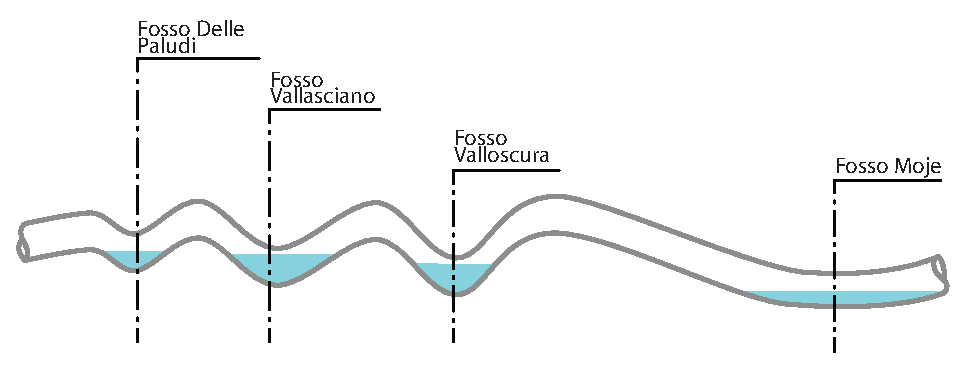
\includegraphics[width=\textwidth]{fig/test/avvallamenti.eps}
    \caption{Rappresentazione schematica dell'acqua localizzata negli abbassamenti di quota della condotta.} 
    \label{fig:acqua-avvallamenti}
\end{figure}

L'obiettivo del trattamento è rimuovere l'acqua accumulata in linea, in particolare nei quattro avvallamenti che, a causa dell'\textit{hold up}, limitano la produzione gas generando una elevata contropressione. L'analisi si baserà sulla valutazione dell'azione dello schiumogeno in condotta e i risultati avuti nel breve-medio termine. Al fine di confermare i vantaggi legati all'applicazione, si fa riferimento all'ultimo piggaggio della linea Verdicchio effettuato nel luglio 2013.

\section{Polo produttivo di San Giorgio Mare}
La centrale di San Giorgio Mare (centrale SGM), collocata nel Comune di Fermo in Località Marina Palmense (FM), è destinata all'attività di produzione, compressione e trattamento di gas naturale ed è stata sviluppata a cavallo tra il 1970 e il 1972. L'impianto rientra nella Business Unit Asset Idrocarburi della Edison S.p.A. ed è gestito dal Distretto Operativo di Sambuceto (CH) che cura inoltre la Direzione di tutte le attività del Sistema di Gestione Integrato dell'Ambiente e della Sicurezza. Il polo produttivo di San Giorgio Mare comprende:
\begin{itemize}
	\item pozzi relativi alle concessioni off-shore di Vongola Mare (VGM1), San Giorgio Mare (SGMC, SGM3, SGM6) e concessioni in-shore Verdicchio (VRD-1), San Marco (SNM1-2-3), Cozza Terra (CZT-2D), Cassiano, Castellaro;
	\item linee di collegamento tra pozzi e centrale SGM;
	\item centrale SGM;
	\item vasche e serbatori di raccolta acque e gasolina;
	\item punti di collegamento con le reti di distribuzione a carattere nazionale (Snam Rete Gas e SGI S.p.A.).
\end{itemize}
La centrale SGM riceve il gas proveniente dai pozzi e le piattaforme off-shore mediante una tubazione sottomarina (\textit{sealine}) da ø 8", dimensione nominale della condotta), e ø 10" dal campo SGM. Il gas proveniente dai campi on-shore arriva in centrale tramite una condotta sotterrata da ø 6" che prende il nome di "linea Verdicchio". 

\begin{figure}[htbp]
	\centering
	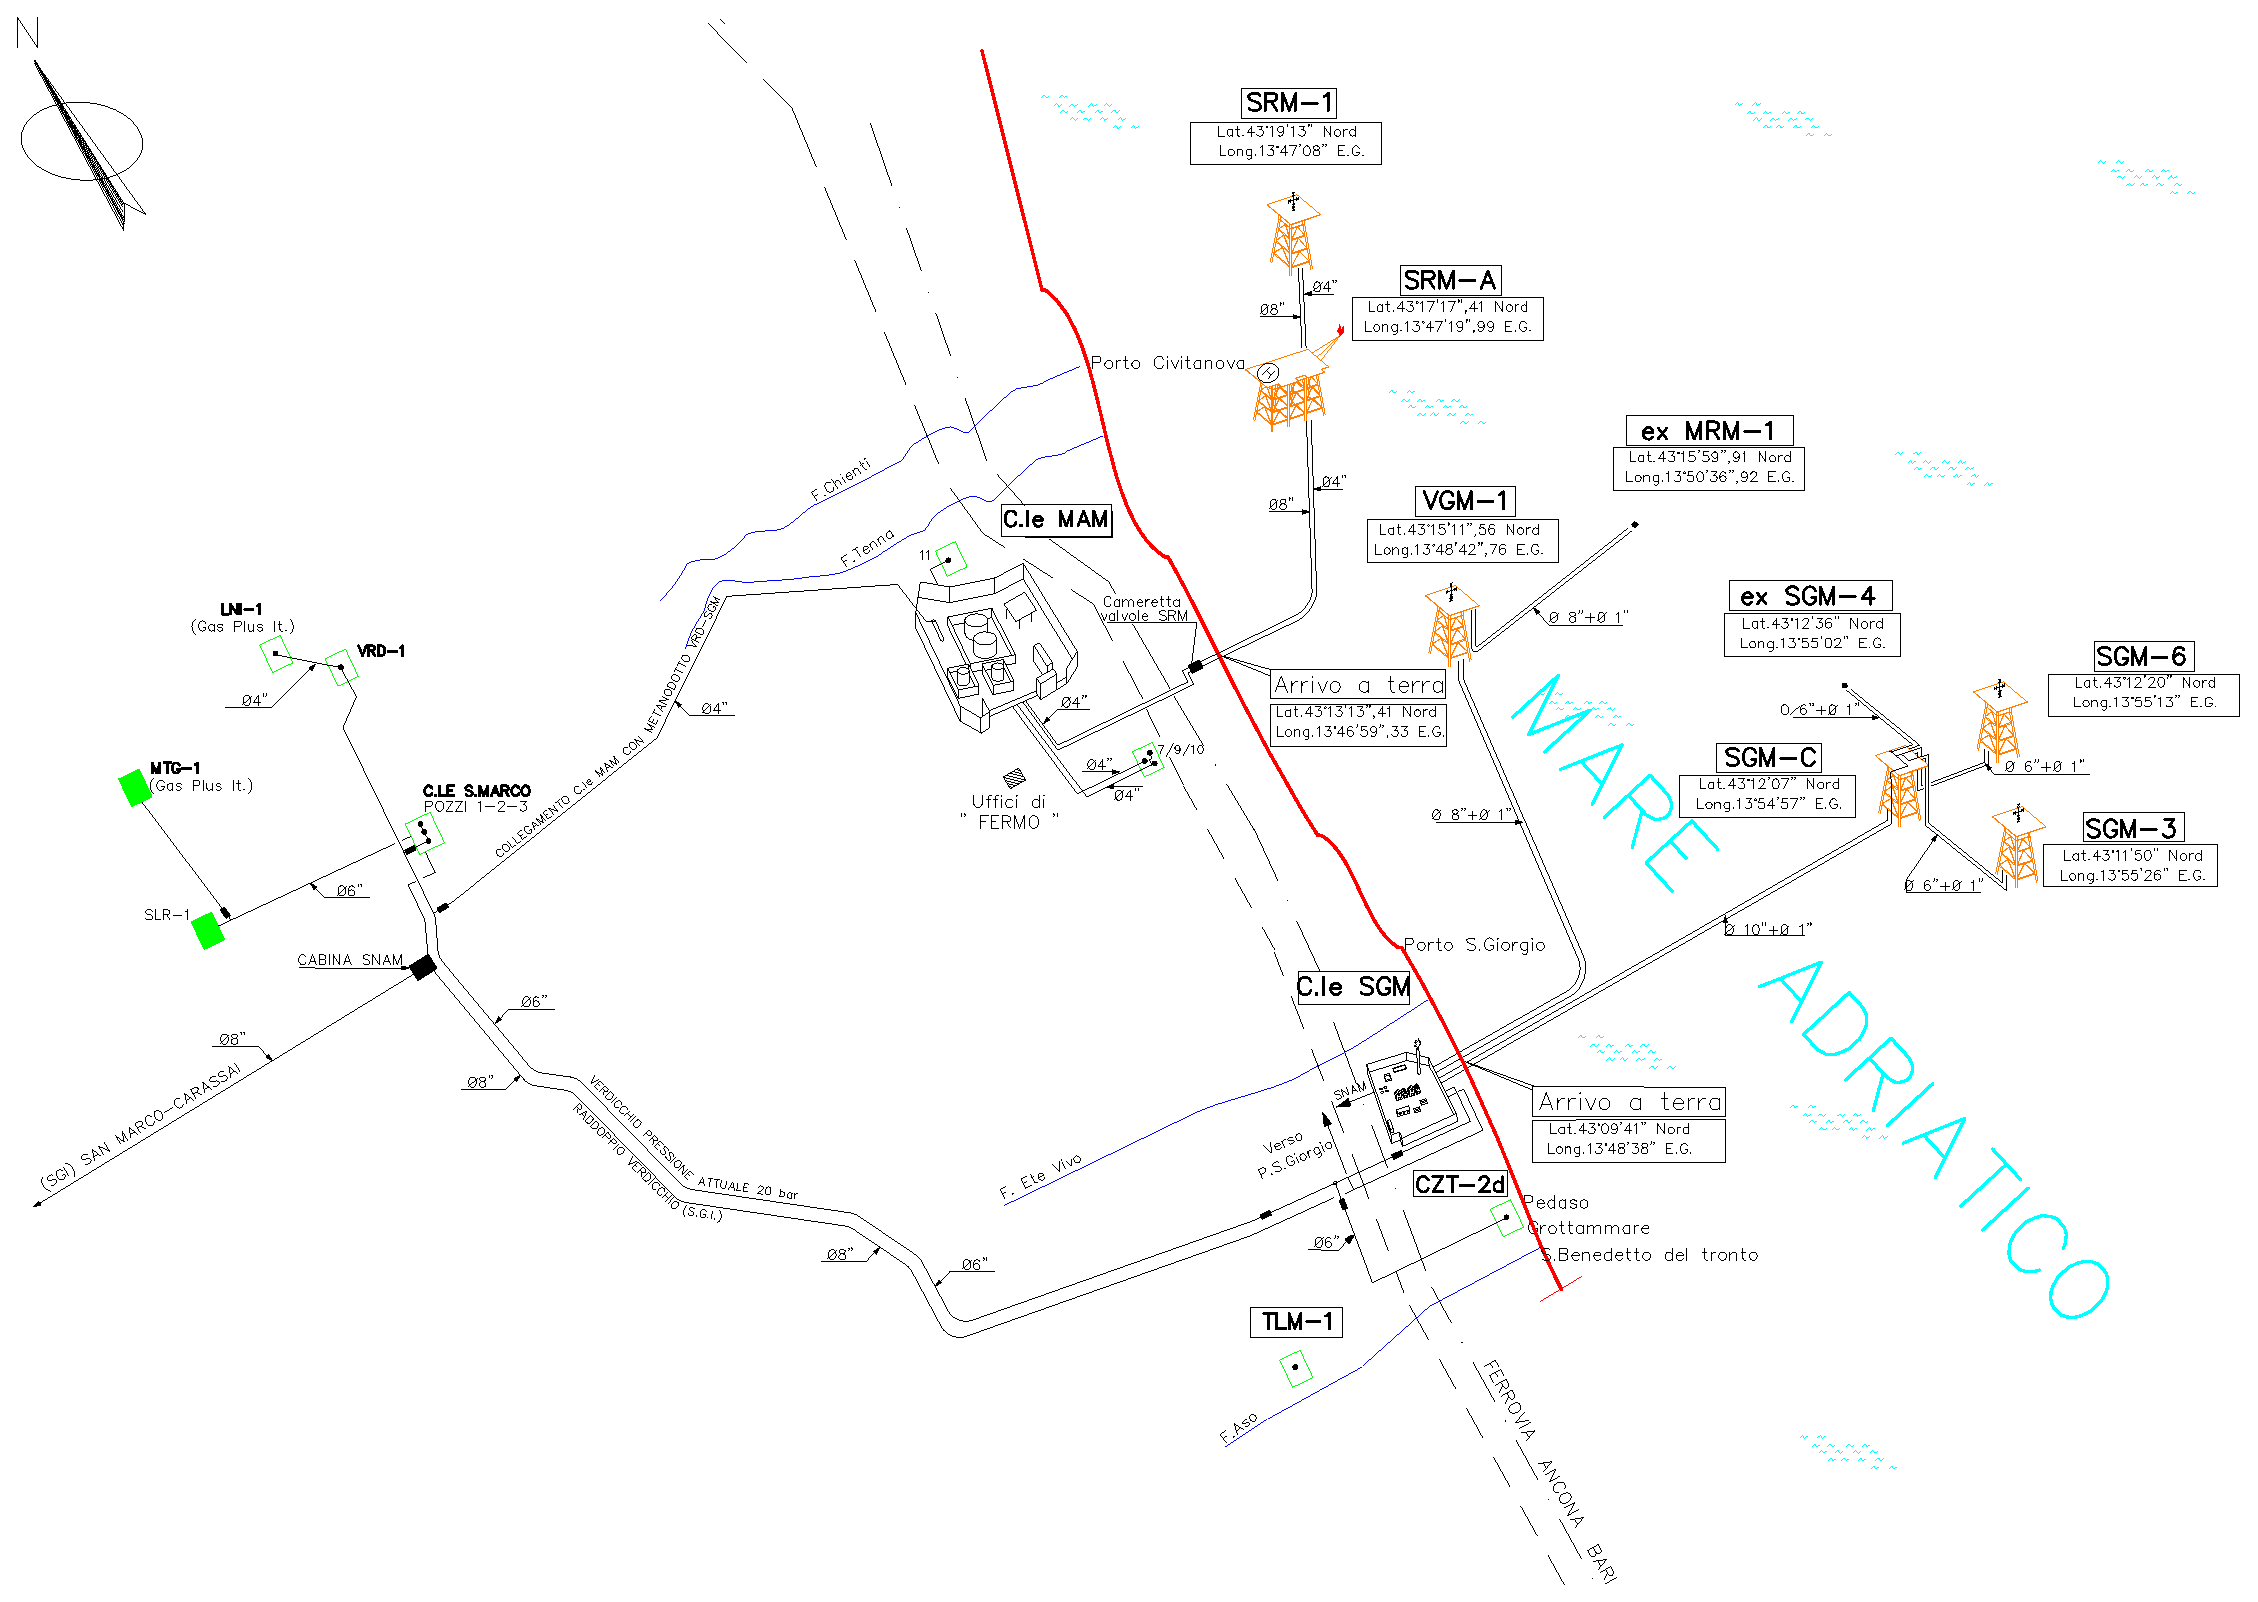
\includegraphics[width=\textwidth]{fig/test/asset.eps}
	\caption{Planimetria delle installazioni on-shore e off-shore relative al polo produttivo di San Giorgio Mare.}
	\label{fig:asset}
\end{figure}

\subsection{La linea Verdicchio}
La linea Verdicchio rappresenta la spina dorsale di tutta la produzione on-shore di gas naturale. La linea ha lunghezza complessiva di 13.600 metri circa e che raccoglie le produzioni dei campi di Verdicchio, San Marco, San Lorenzo e Cozza Terra, e la produzione dei campi Leoni e Monte Guzzo della società Gas Plus S.p.A., ora improduttivi.  Nel 2013 la centrale MAM è stata collegata alla \textit{flow line} di Verdicchio tramite una condotta da ø 4", convogliando il gas di coda proveniente dai campi olio Sarago Mare e Santa Maria a Mare. Il gas derivante da espansione viene inviato tramite compressione.\\

\begin{figure}[htbp]
	\centering
	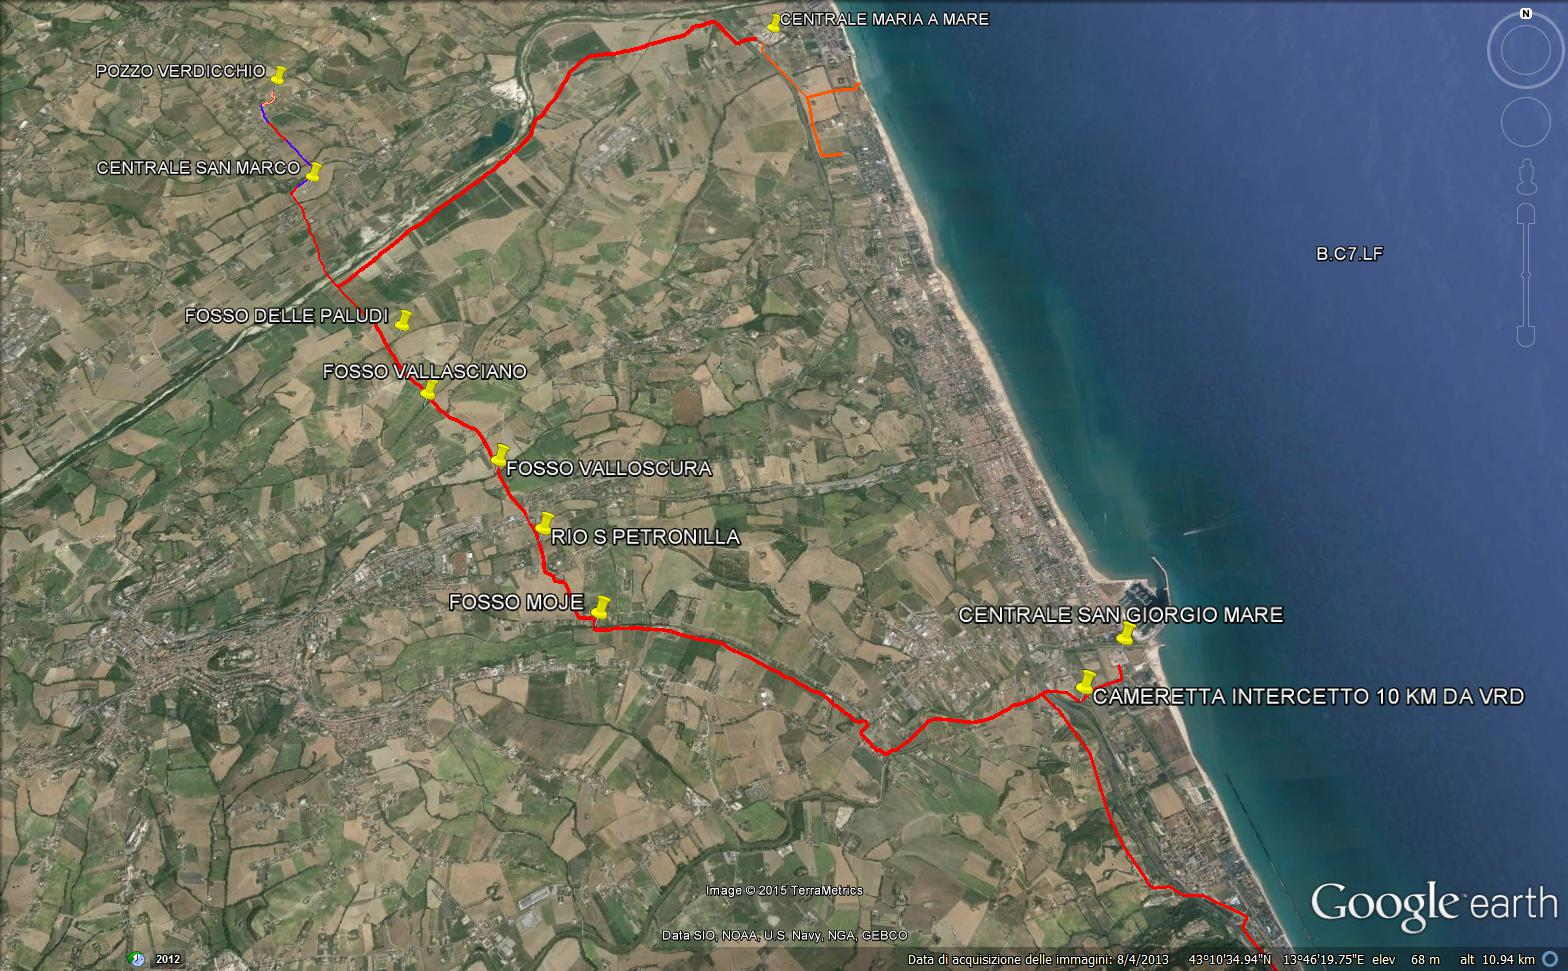
\includegraphics[width=\textwidth]{fig/test/linea-verdicchio}
	\caption{Aree pozzo e avvallamenti attraversati dalla linea Verdicchio.}
	\label{fig:lineavrd}
\end{figure}

Il territorio su cui è collocata la rete di distribuzione interna è di natura collinare, di conseguenza il profilo della condotta è caratterizzato da variazioni di quota (\figref{fig:quota-linea-vrd}). La condotta parte dall'omonima area pozzo e passa attraverso l'area produttiva di San Marco. In questo punto la linea Verdicchio è collegata al polo di San Lorenzo, il quale immette il gas prodotto. Di seguito la condotta oltrepassa quattro diversi avvallamenti: Fosso delle Paludi, Fosso Vallasciano, Fosso Valloscura e Fosso Moje, con variazioni di quota fino a 80 metri. Poco prima dell'arrivo in centrale, un raccordo proveniente da Sud permette l'immissione del gas proveniente da Cozza, la cui produzione però è attualmente ferma.

\begin{figure}[htbp]
	\centering
    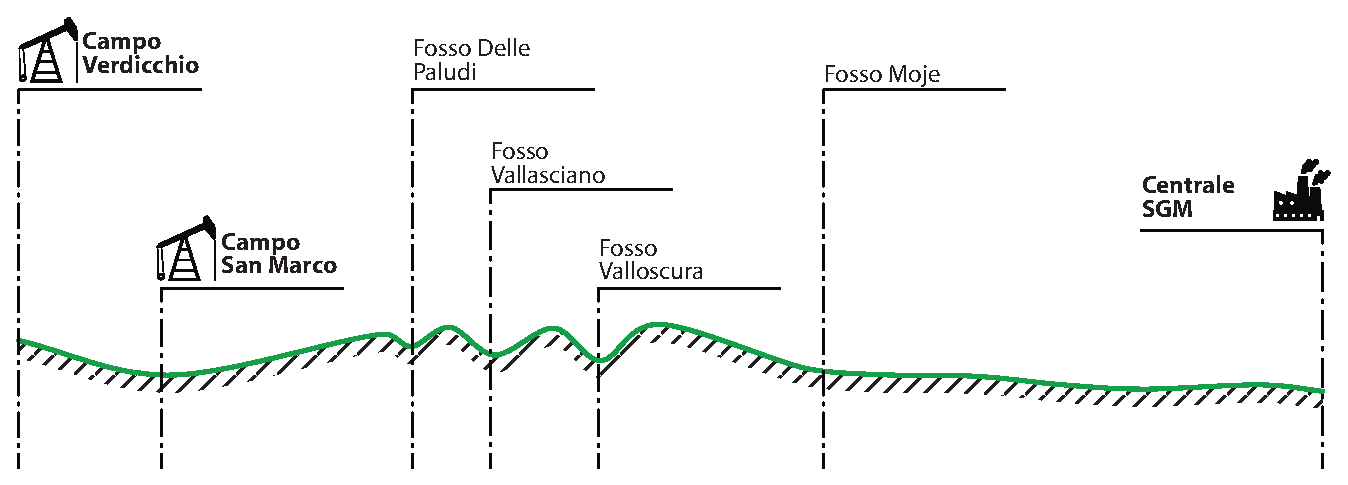
\includegraphics[width=\textwidth]{fig/test/linea-vrd-quota.eps}
 	\caption{Variazioni di quota lungo la linea Verdicchio.}
 	\label{fig:quota-linea-vrd}
\end{figure}

Qui di seguito sono descritte i campi di Verdicchio e di San Marco. Nel seguente lavoro si è deciso di trascurare San Lorenzo poiché la pressione di testa pozzo di SL-1B (circa 96 bar) è al di sopra della pressione critica, perciò qualsiasi variazione della pressione in condotta non influenza le condizioni di produzione del sito in questione
\footnote{La pressione critica rappresenta il valore per il quale vengono raggiunte le condizioni critiche di una corrente gassosa \parencite{sabetta2009gasdinamica}. In questa fase la velocità del fluido è pari alla velocità del suono, velocità con cui una perturbazione si propaga in tale fluido. Se la pressione di monte è al di sopra della pressione critica mentre la pressione di valle è al di sotto, l'informazione di una eventuale variazione delle condizioni di valle (e.g. perturbazione dovuta a un restringimento e/o ostacolo) non è in grado di procedere verso monte.}
.

\subsection{Campo Verdicchio}
Il campo è costituito da un solo pozzo VRD-1 e il gas prodotto viene trasferito, senza alcun trattamento tramite una condotta da ø 6" alla centrale San Giorgio Mare per il trattamento e la compressione.\\
Sull'area sono presenti cabina elettrica, serbatoio aria compressa per la strumentazione collegato al compressore di alimentazione e trappola di lancio pig di pulizia della linea Verdicchio dall'area pozzo omonima alla centrale SGM.\\
Il piazzale è recintato e nella recinzione esiste la seconda uscita di sicurezza, il pozzo ha la gabbia di testa con doppia apertura ed è dotata di scarico a terra.

\begin{figure}[htbp]
	\centering
	\subfloat[][Ortofoto.]
    {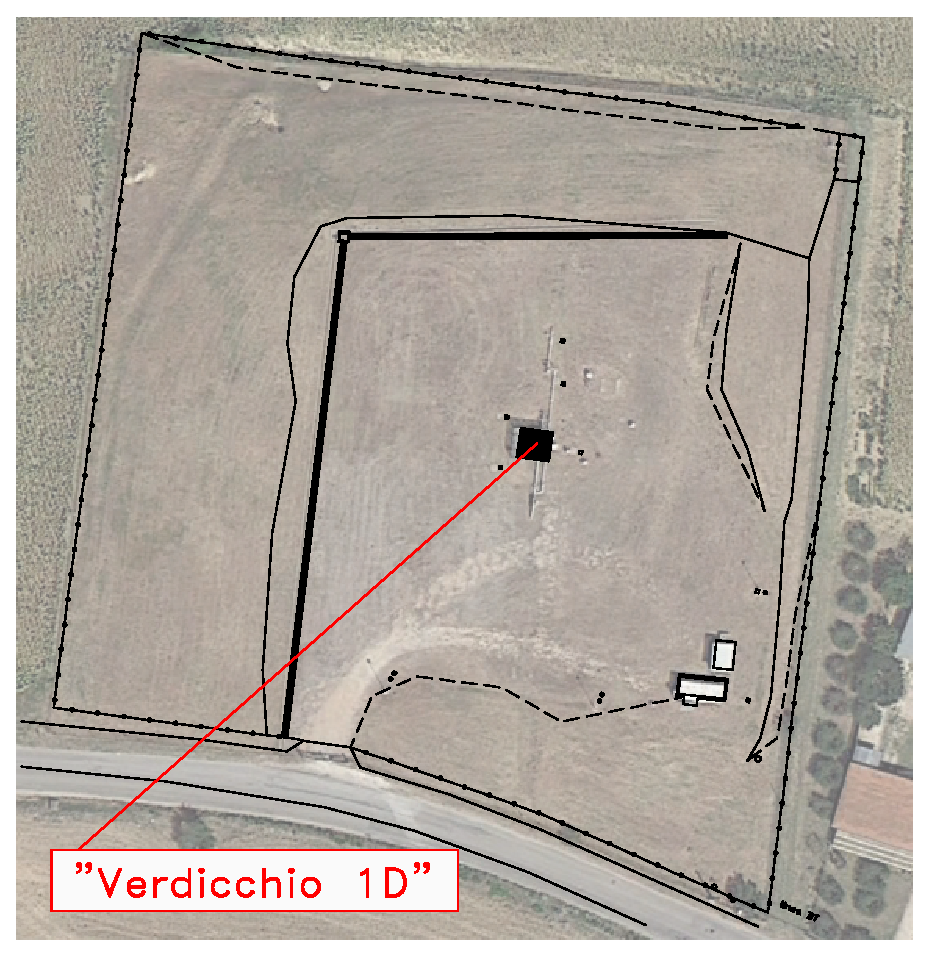
\includegraphics[height=.25\textheight]{fig/test/verdicchio-1.eps}  \label{fig:vrd-1}} \qquad
	\subfloat[][Testa pozzo.]
    {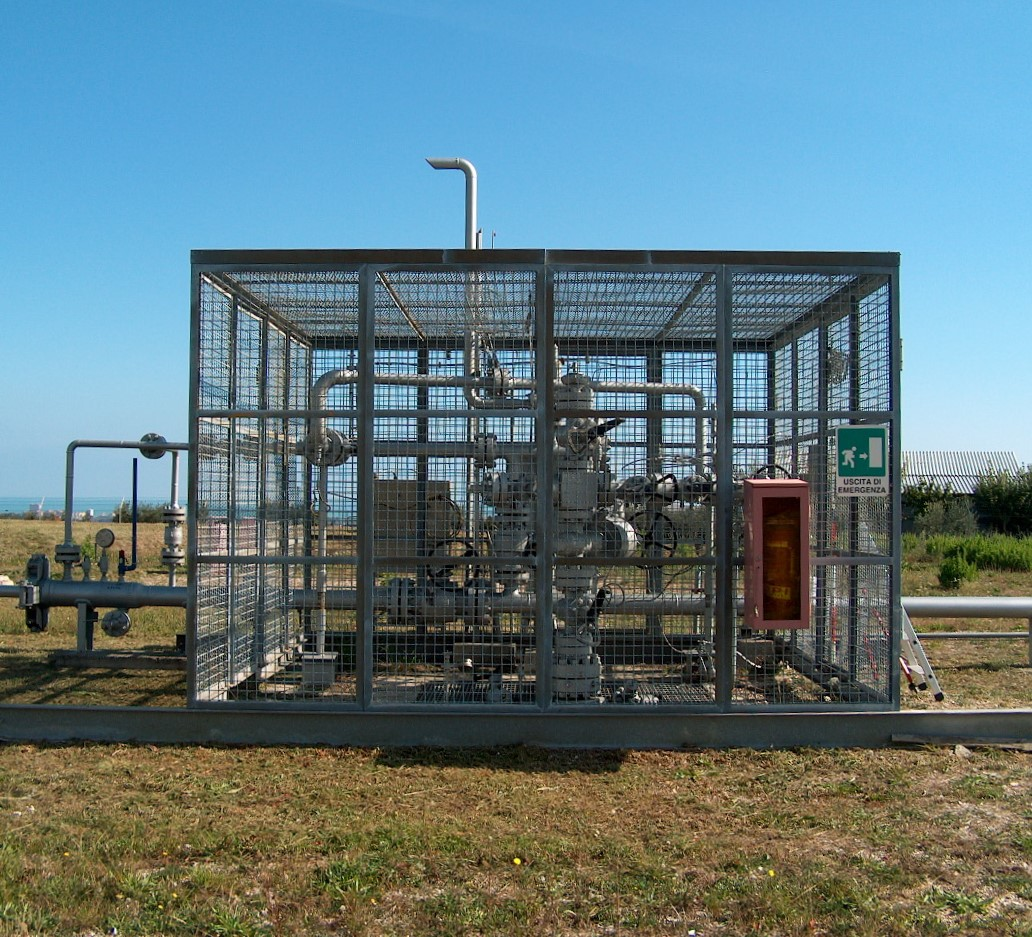
\includegraphics[height=.25\textheight]{fig/test/verdicchio-2}  \label{fig:vrd-2}}
 	\caption{Area pozzo di Verdicchio.}
 	\label{area-vrd}
\end{figure}

\subsection{Campo San Marco}
Il campo è costituito da tre pozzi: SNM-1 (a 2 stringhe), SNM-2 (a 4 stringhe, di cui 2 attualmente ferme) e SNM-3 (a 2 stringhe).
In origine il gas in uscita dai separatori veniva riscaldato, ridotto di pressione, misurato. Con la diminuzione fisiologica dell'energia di giacimento, quindi delle pressioni, il gas in uscita dai separatori non necessita di disidratazione spinta e viene inviato direttamente alla linea di Verdicchio per il trattamento definitivo alla centrale SGM.\\
L'area operativa di San Marco ha la struttura di una centrale costituita da strutture di servizio (dove si svolgono le operazioni di gestione e coordinamento dal campo e dove sono registrate le misure fiscali e non del gas in uscita), officina meccanica e strumentale, magazzino, apparati di distribuzione dell'energia elettrica (cabina elettrica, inverter con batterie e quadri di distribuzione delle utenze) e l'impianto di trattamento, il quale è parzialmente in quiescenza.\\
Le acque di strato prodotte dalla coltivazione dei pozzi provenienti dai separatori vengono raccolte in delle vasche. Queste acque sono poi periodicamente caricate, trasportate e immesse nei pozzi iniettori MAT-11 e MAT-7 della centrale di Maria a Mare (MAM).

\begin{figure}[htbp]
	\centering
	\subfloat[][Ortofoto.]
    {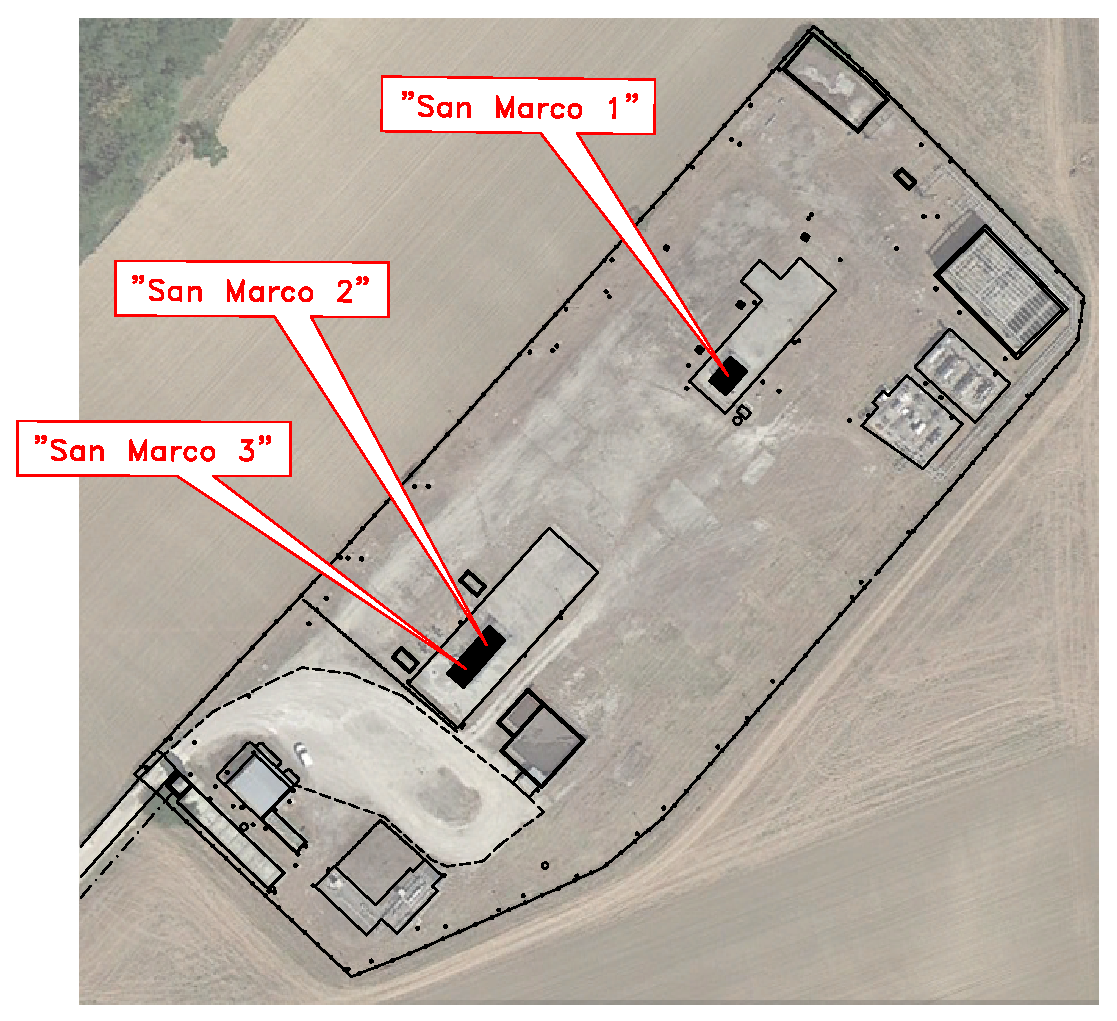
\includegraphics[height=.25\textheight]{fig/test/snm-1.eps}  \label{fig:snm-1}} \qquad
	\subfloat[][Testa pozzo SNM-1.]
   {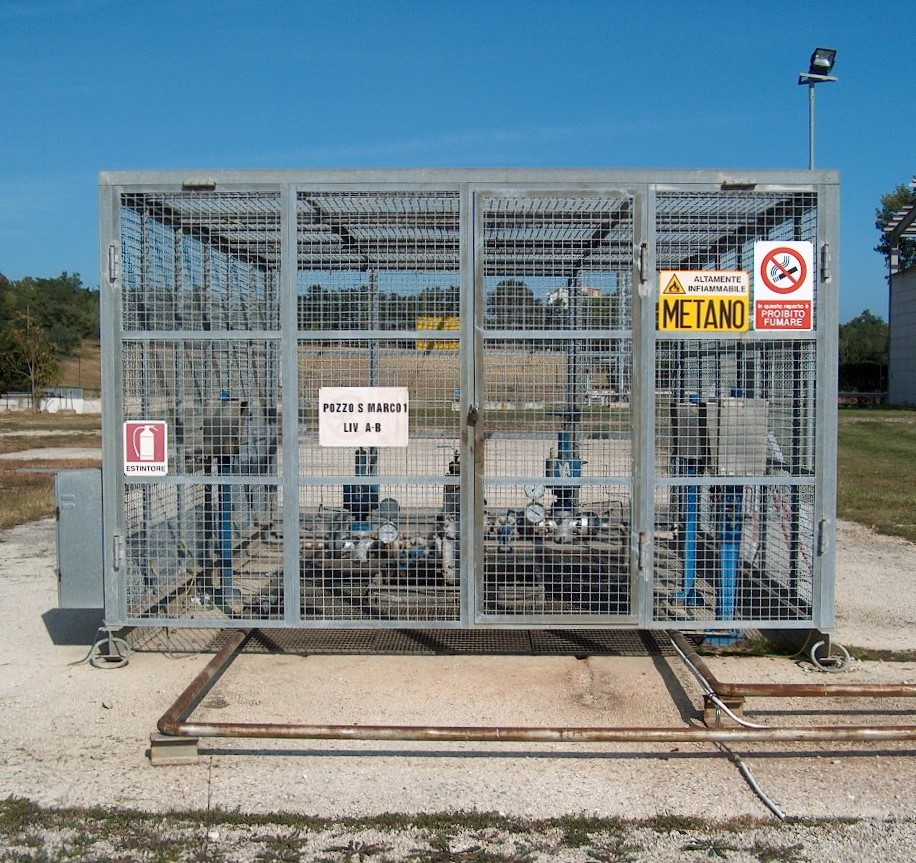
\includegraphics[height=.25\textheight]{fig/test/snm-2}  \label{fig:snm-2}}
 	\caption{Area pozzo di San Marco.}
 	\label{area-snm}
\end{figure}

\subsection{La centrale di San Giorgio Mare}
La centrale SGM si trova nel cuore del polo produttivo di San Giorgio Mare, nella Località Marina Palmense (FM), a circa 300 m di distanza dalla costa e 200 m dall'autostrada A14. L'area complessiva interessata è di circa 30.000 m\ap{2}, di cui 300 m\ap{2} dedicata agli uffici e alla sala controllo.
Le principali attività svolte dal polo produttivo di San Giorgio Mare sono:
\begin{itemize}
 	\item produzione di gas dal giacimento;
 	\item separazione dell'acqua e gasolina (principalmente dal pozzo SGM6) associate al gas naturale;
 	\item stoccaggio e spedizione dell'acqua di strato;
 	\item compressione del gas naturale;
 	\item disidratazione del gas naturale;
 	\item vendita del gas naturale, previa misura fiscale.
\end{itemize}

\begin{figure}
    \centering
    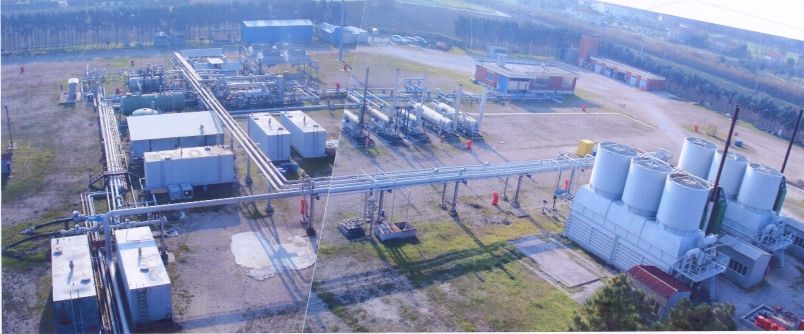
\includegraphics[width=\textwidth]{fig/test/centrale/sgm-alto}
    \caption{Vista dall'alto della centrale di San Giorgio Mare.}
    \label{fig:sgm-alto}
\end{figure}

\subsubsection*{Separatori}
I separatori S-101, S-111, S-112 sono separatori orizzontali, S-101 e S-111 sono separatori bifase mentre S-112 è un separatore trifase, dedicato al gas a condensati proveniente dai campi off-shore di San Giorgio Mare. La geometria dei separatori è diversa e va da un volume minimo di 2.100 l (S-101) a un massimo di 10.500 l (S-111). L'acqua di strato viene inviata tramite autobotti alla centrale MAM e pompata nei pozzi di reiniezione, come previsto da autorizzazione. La gasolina proveniente dal solo separatore S-112 è inviata all'impianto di trattamento dedicato.
La regolazione dei rispettivi livelli avviene tramite valvole di controllo livello (LCV, \textit{Level Control Valve}), mentre la pressione dei separatori è regolata tramite la valvola di controllo della pressione (PCV, \textit{Pressure Control Valve}).
\begin{figure}[htbp]
    \centering
    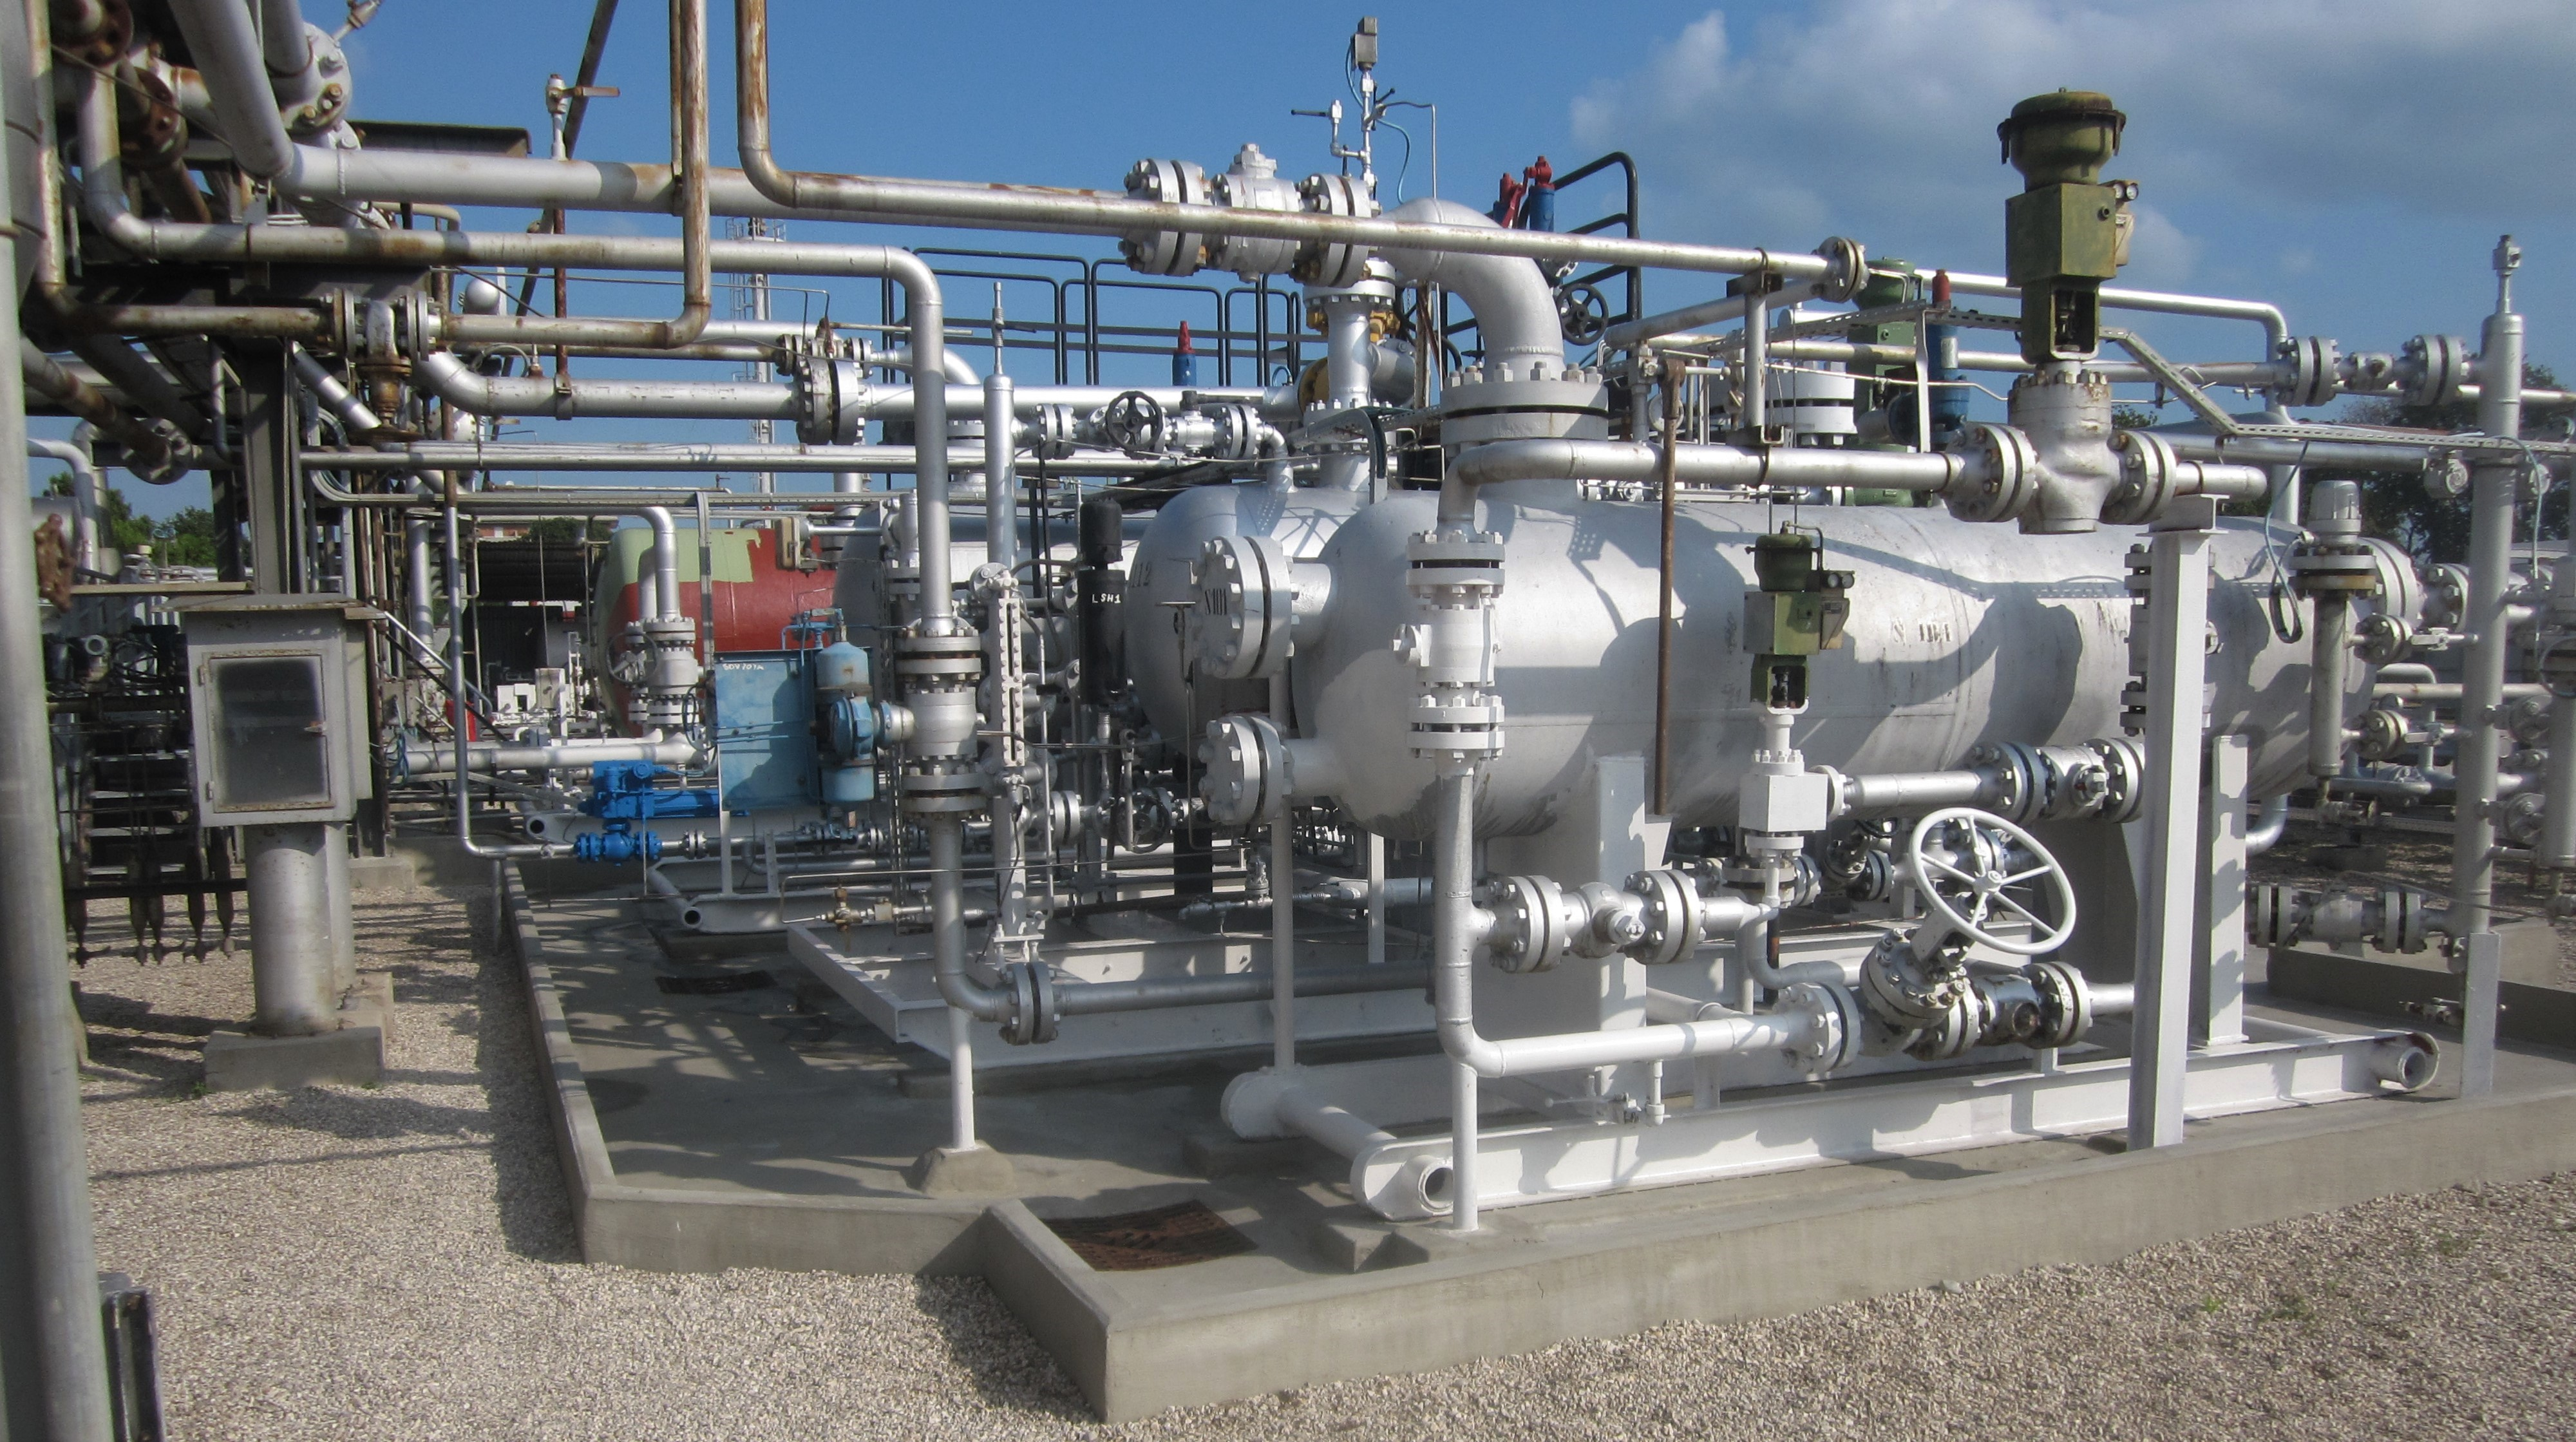
\includegraphics[width=.7\textwidth]{fig/test/centrale/separatori}
    \caption{Separatori a monte di tutto il trattamento gas.} 
    \label{fig:centrale-separatore}
\end{figure}

\subsubsection*{Compressione}
L'impianto di compressione è costituito da:
\begin{itemize}
	\item \textbf{compressore} (K-101 e K-201): motocompressori alternativi (monsotadio a doppio effetto) della Nuovo Pignone. I cilindri sono lubrificati e il raffreddamento è ad acqua. Ogni compressore lavora con un rapporto di compressione di 1:3 e sono configurati in serie in modo tale da portare la pressione da 5-7 bar a 45-60 bar.
	\item \textbf{motore compressore}: motore Waukesha (General Electric) endodermico a ciclo Otto alimentato a gas, cilindrata totale da 115.400 cm\ap{3}. La potenza della macchina è di 1547 BHP (\textit{British Horse Power}, cavallo vapore britannico) a 1200 RPM (\textit{Revolutions Per Minute}, giri al minuto);
	\item \textbf{aerorefrigerante} (A-101 e A-201): impianto di raffreddamento ad aria della Nuovo Pignone che raffredda il gas una volta compresso. L'aerorefrigerante è costituito oltre che dalla sezione di refrigerazione del gas di processo anche da due sezioni per la refrigerazione delle acque ausiliarie.
\end {itemize}

\begin{figure}[htbp] %%% Immagine pompa dosatrice
    \centering
    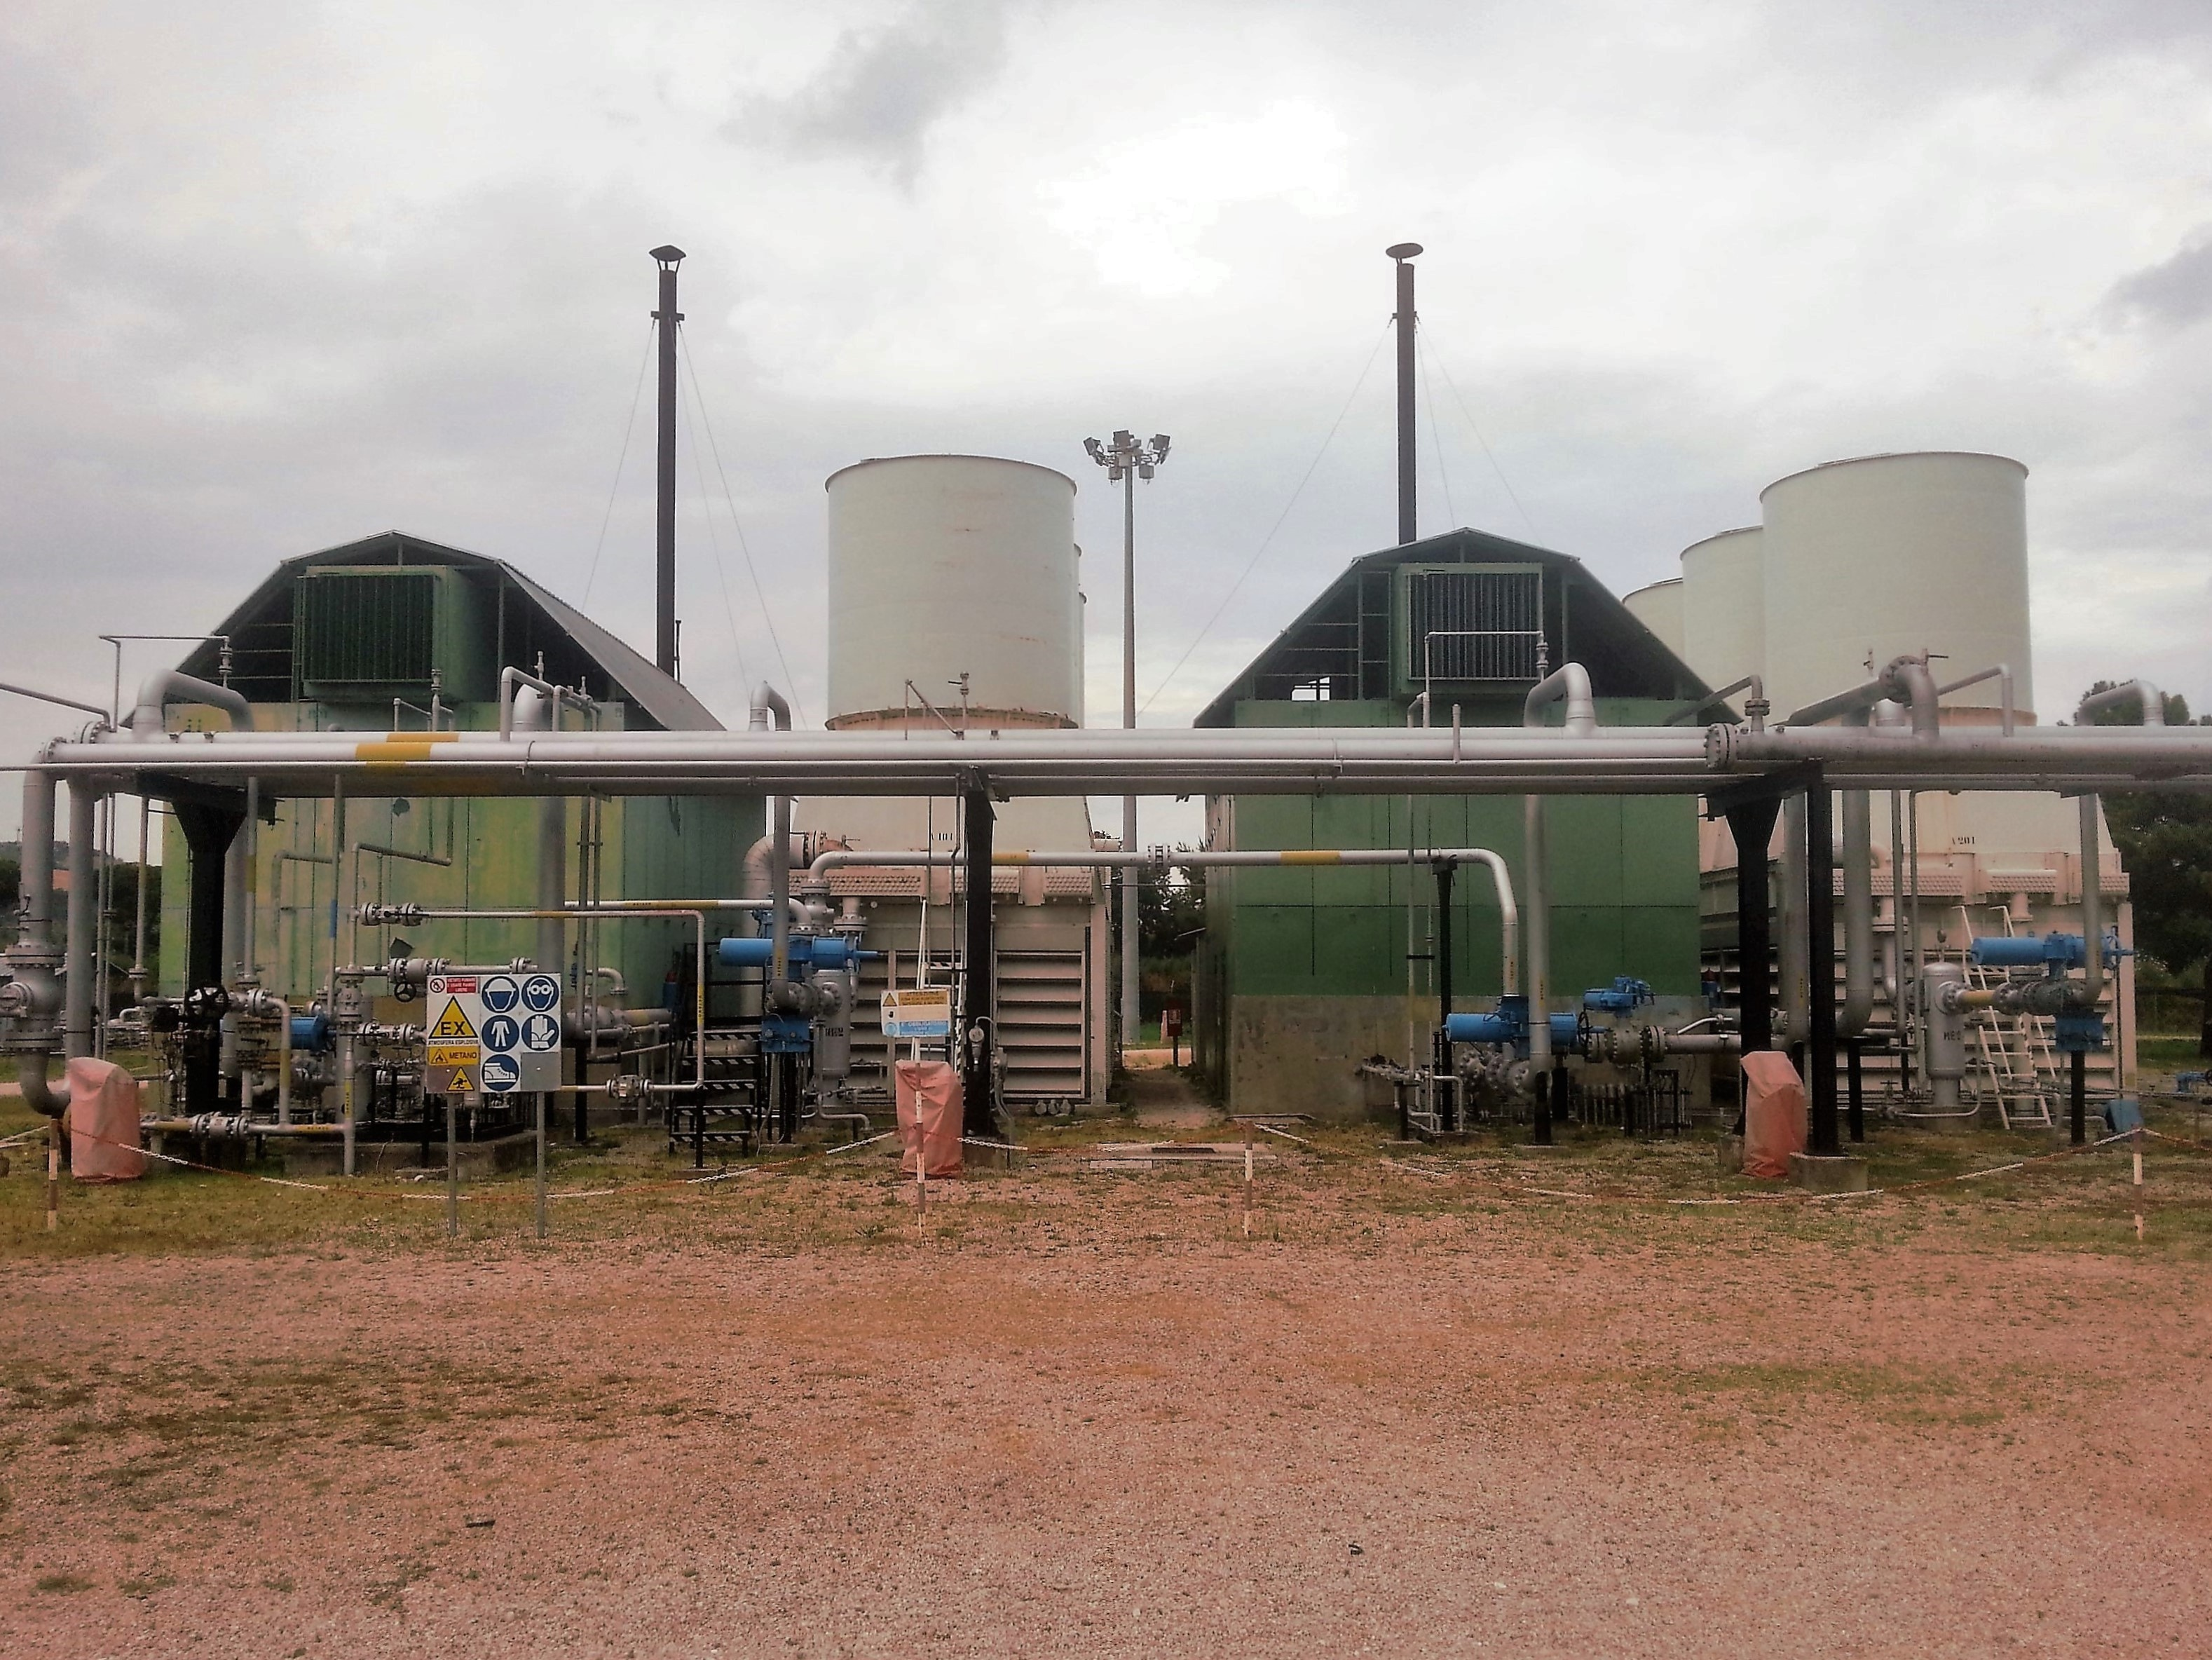
\includegraphics[width=.8\textwidth]{fig/test/centrale/compressori2.jpg} \label{fig:compressionegenerale}
    \caption{Vista da Sud dell'impianto di compressione: in verde gli stabili ospitanti i compressori, in bianco gli impianti di raffreddamento ad aria.} 
    \label{fig:centrale-compressione}
\end{figure}

%\begin{figure}[htbp]
%    \centering
%    \subfloat[][Vista da Sud dell'impianto di compressione complessivo.]
%    {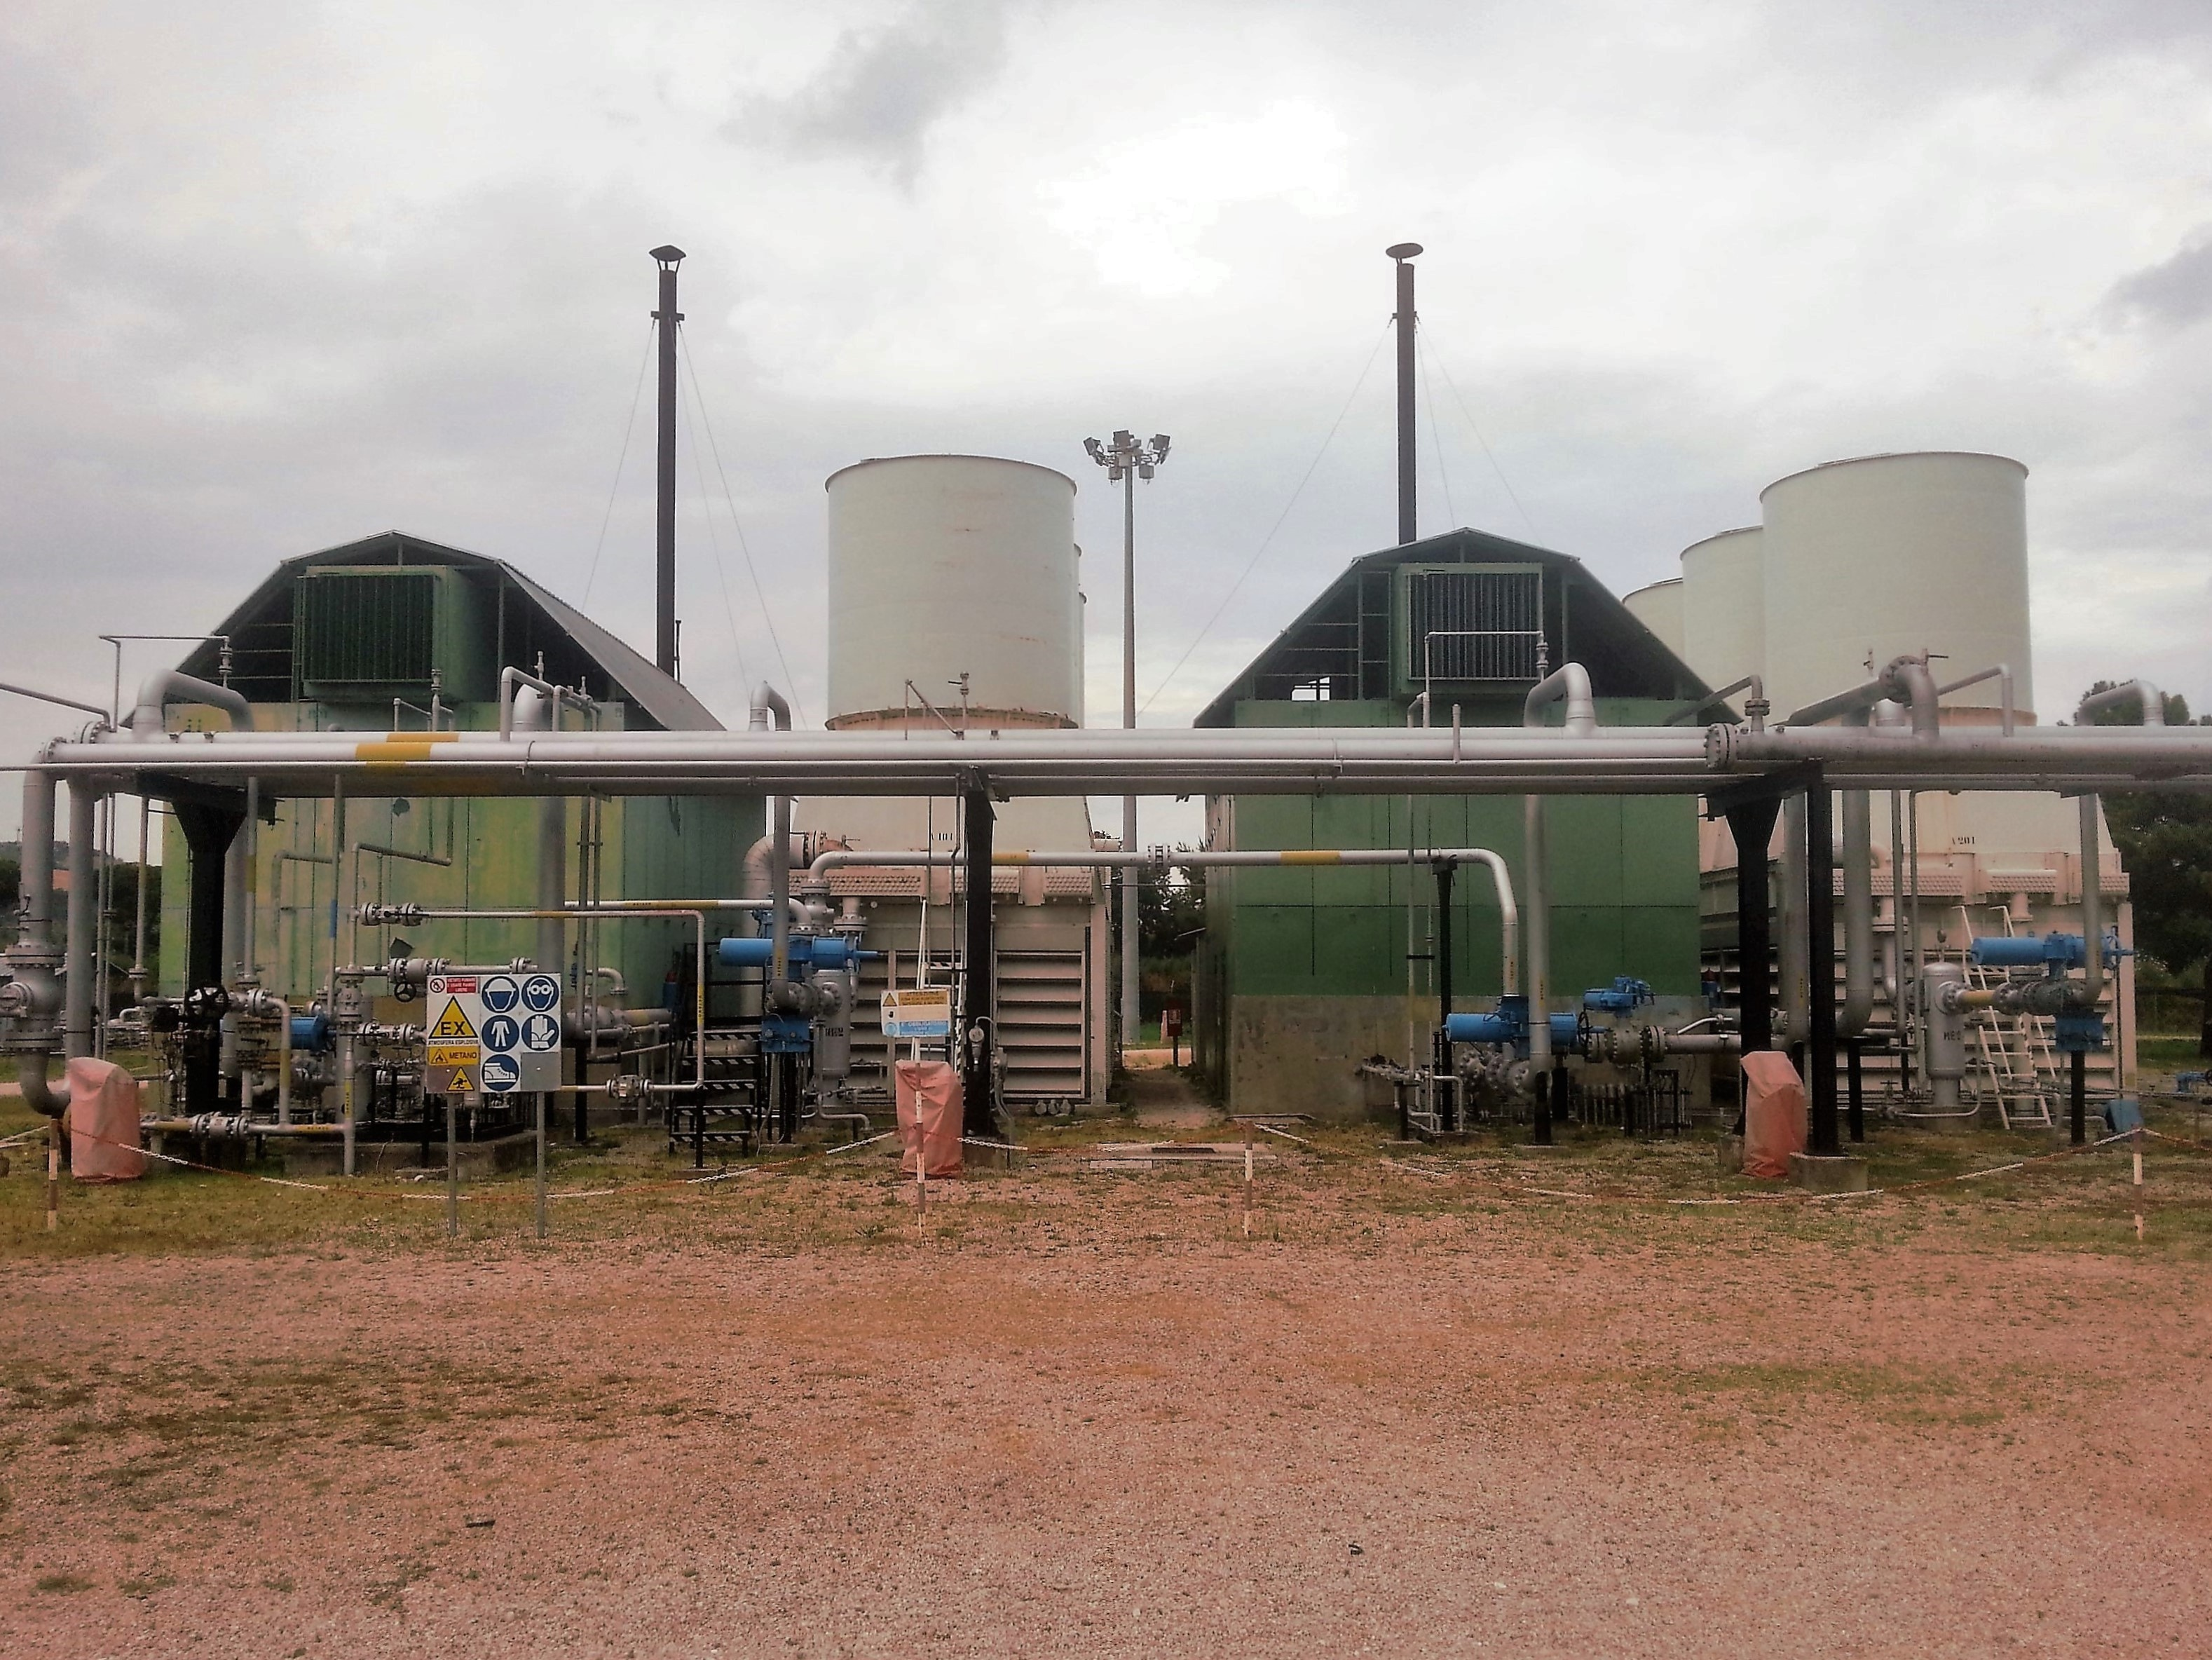
\includegraphics[width=\textwidth]{fig/test/centrale/compressori2.jpg} \label{fig:compressionegenerale}}\\
%    \subfloat[][Impianto di raffreddamento ad aria A-201.]
%    {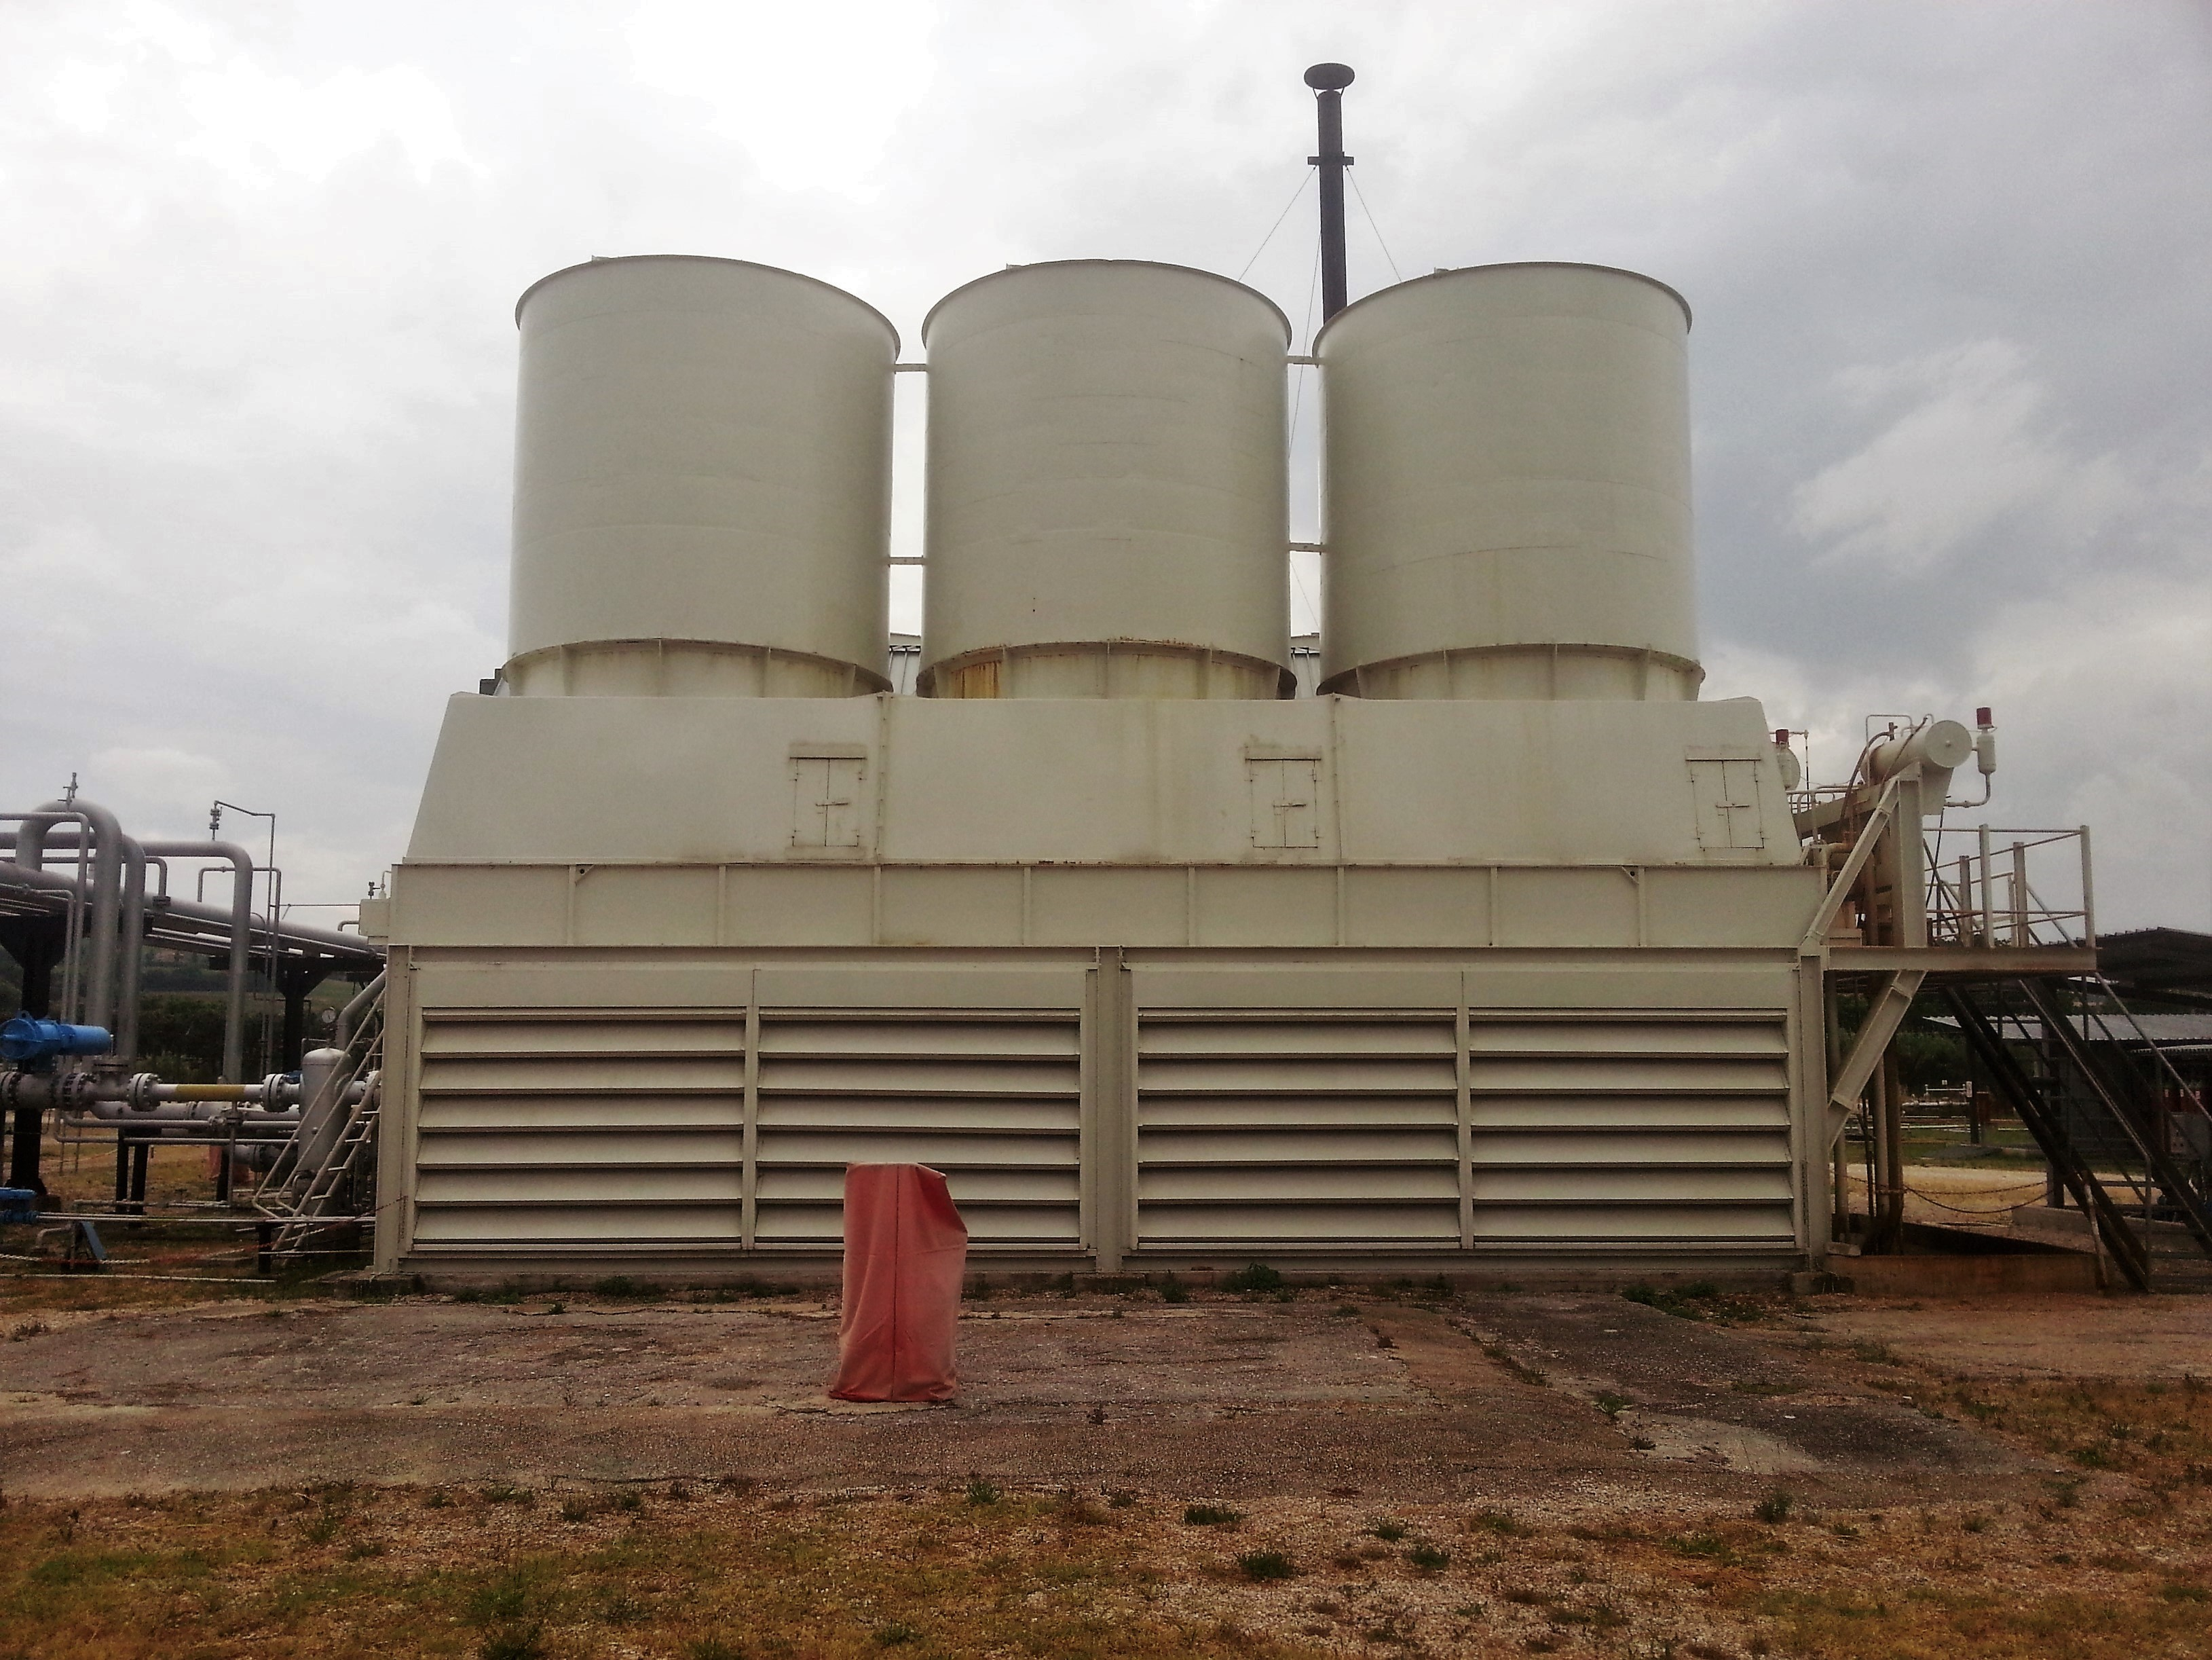
\includegraphics[width=.45\textwidth]{fig/test/centrale/compressori1.jpg} \label{fig:compressioneraffreddamento}} \qquad
%    \subfloat[][Compressore K-201.]
%    {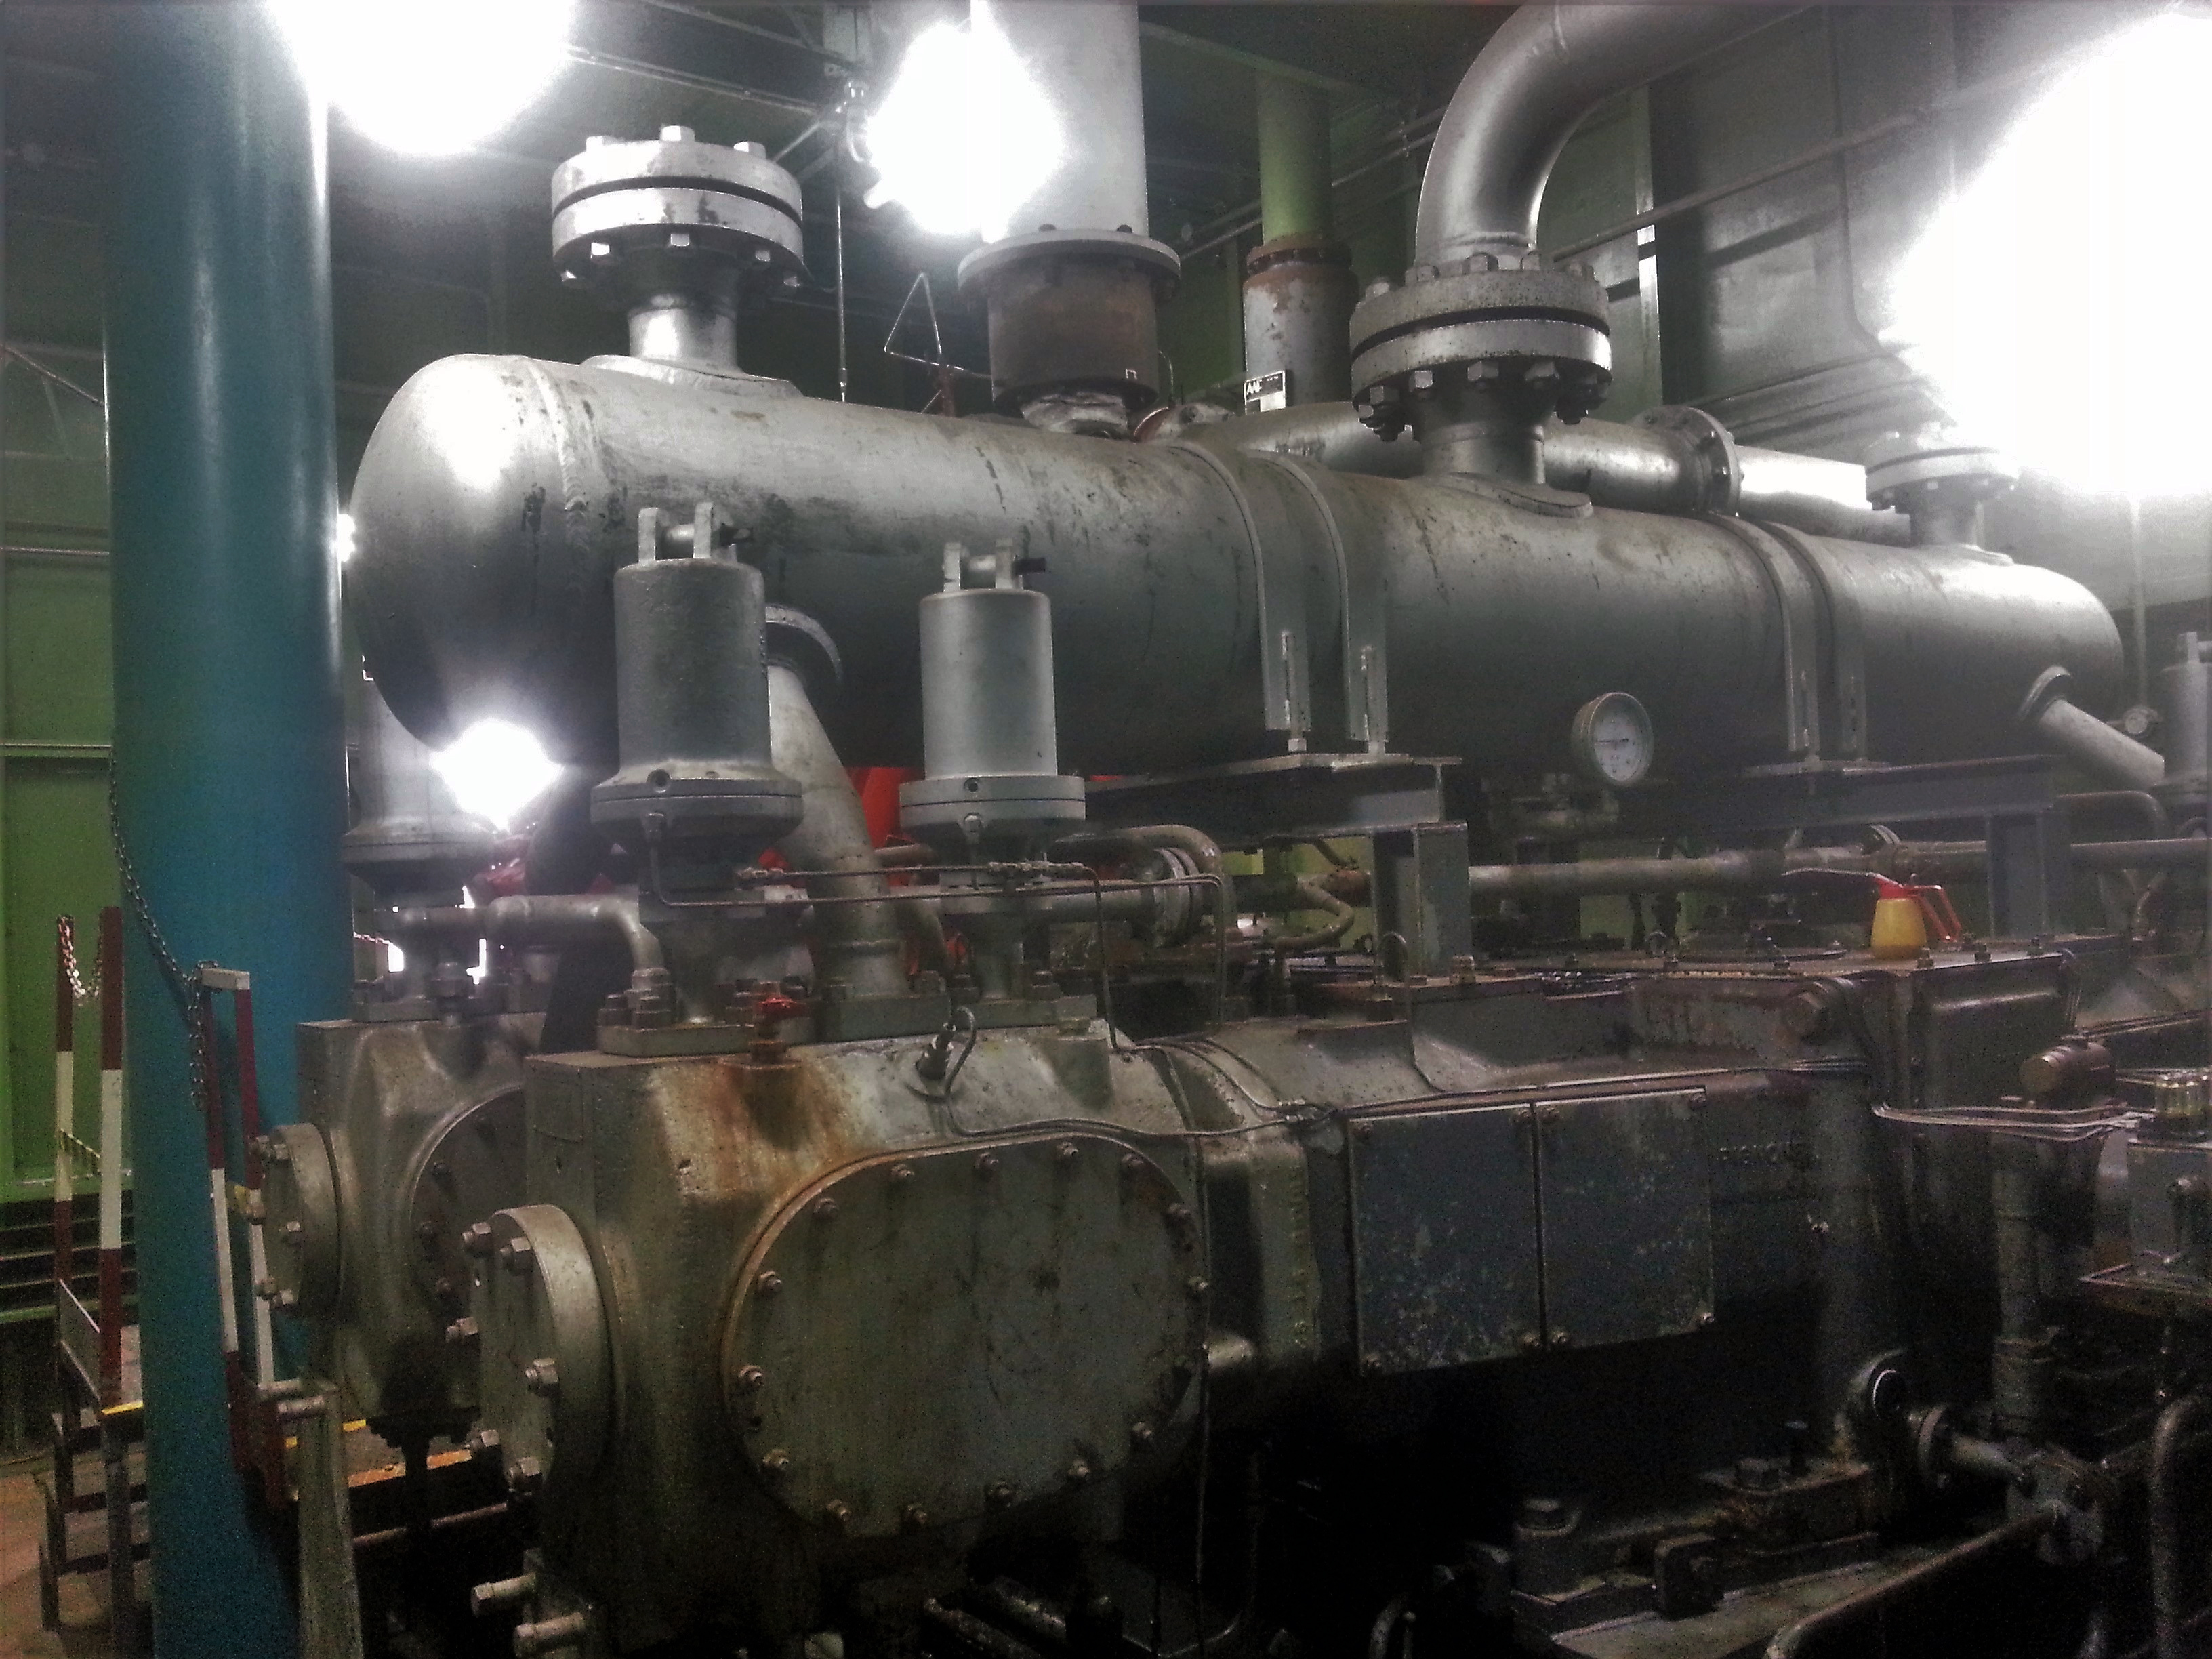
\includegraphics[width=.45\textwidth]{fig/test/centrale/compressori4.jpg} \label{fig:compressa}}   
%\caption{Impianto di compressione del gas naturale, centrale SGM.}
%\label{fig:centrale-compressione}
%\end{figure}


\subsubsection*{Unità di condensazione a bassa temperatura}
La disidratazione e degasolinaggio avviene a opera di un unità di condensazione a bassa temperatura. L'impianto è del tutto equivalente a un LTS convenzionale, nel quale però uno scambiatore gas-freon associato a unità frigorifera svolge gran parte dell'azione refrigerante, dato che le pressioni in ingresso in centrale non sono sufficienti a garantire un adeguato raffreddamento per espansione. L'unità di condensazione è costituita da:
\begin{itemize}
	\item \textbf{scambiatore gas/gas}: costituito da due cilindri da 16" di diametro e 24 ft di lunghezza in serie, superficie di scambio totale di 162 m\ap{2}, il gas viene pre-raffreddato tramite scambio termico con il gas freddo in uscita dall'unità, il quale viene a sua volta riscaldato in uscita dall'unità di condensazione;
	\item \textbf{valvola di iniezione glicol}: all'ingresso dell'unità, utile a inibire la formazione di idrati se la temperatura scende al di sotto del punto di formazione;
	%\item \textbf{duse di espansione}: raffredda il flusso tramite controllo pressione e semplice espansione del gas;
	\item \textbf{scambiatore gas-freon}: l' evaporatore o \textit{chiller}, accoppiato con un unità frigorifero, premette il raggiungimento della temperatura finale di -15°C\footnote{La temperatura è calcolata sul diagramma di fase: per una pressione di 45 bar (pressione in uscita dall'unità di compressione), il punto di rugiada si trova a -5°C};
	\item \textbf{trappola di idrati}: placca forata verticalmente posta in verticale nel separatore;
	\item \textbf{separatore orizzontale a bassa temperatura}: separatore a freddo bifasico di 26" di diametro, l'evacuazione del liquido è controllata da una valvola di regolazione livello (\textit{level control valve}, LCV).
\end{itemize}

\begin{figure}[htbp] 
    \centering
    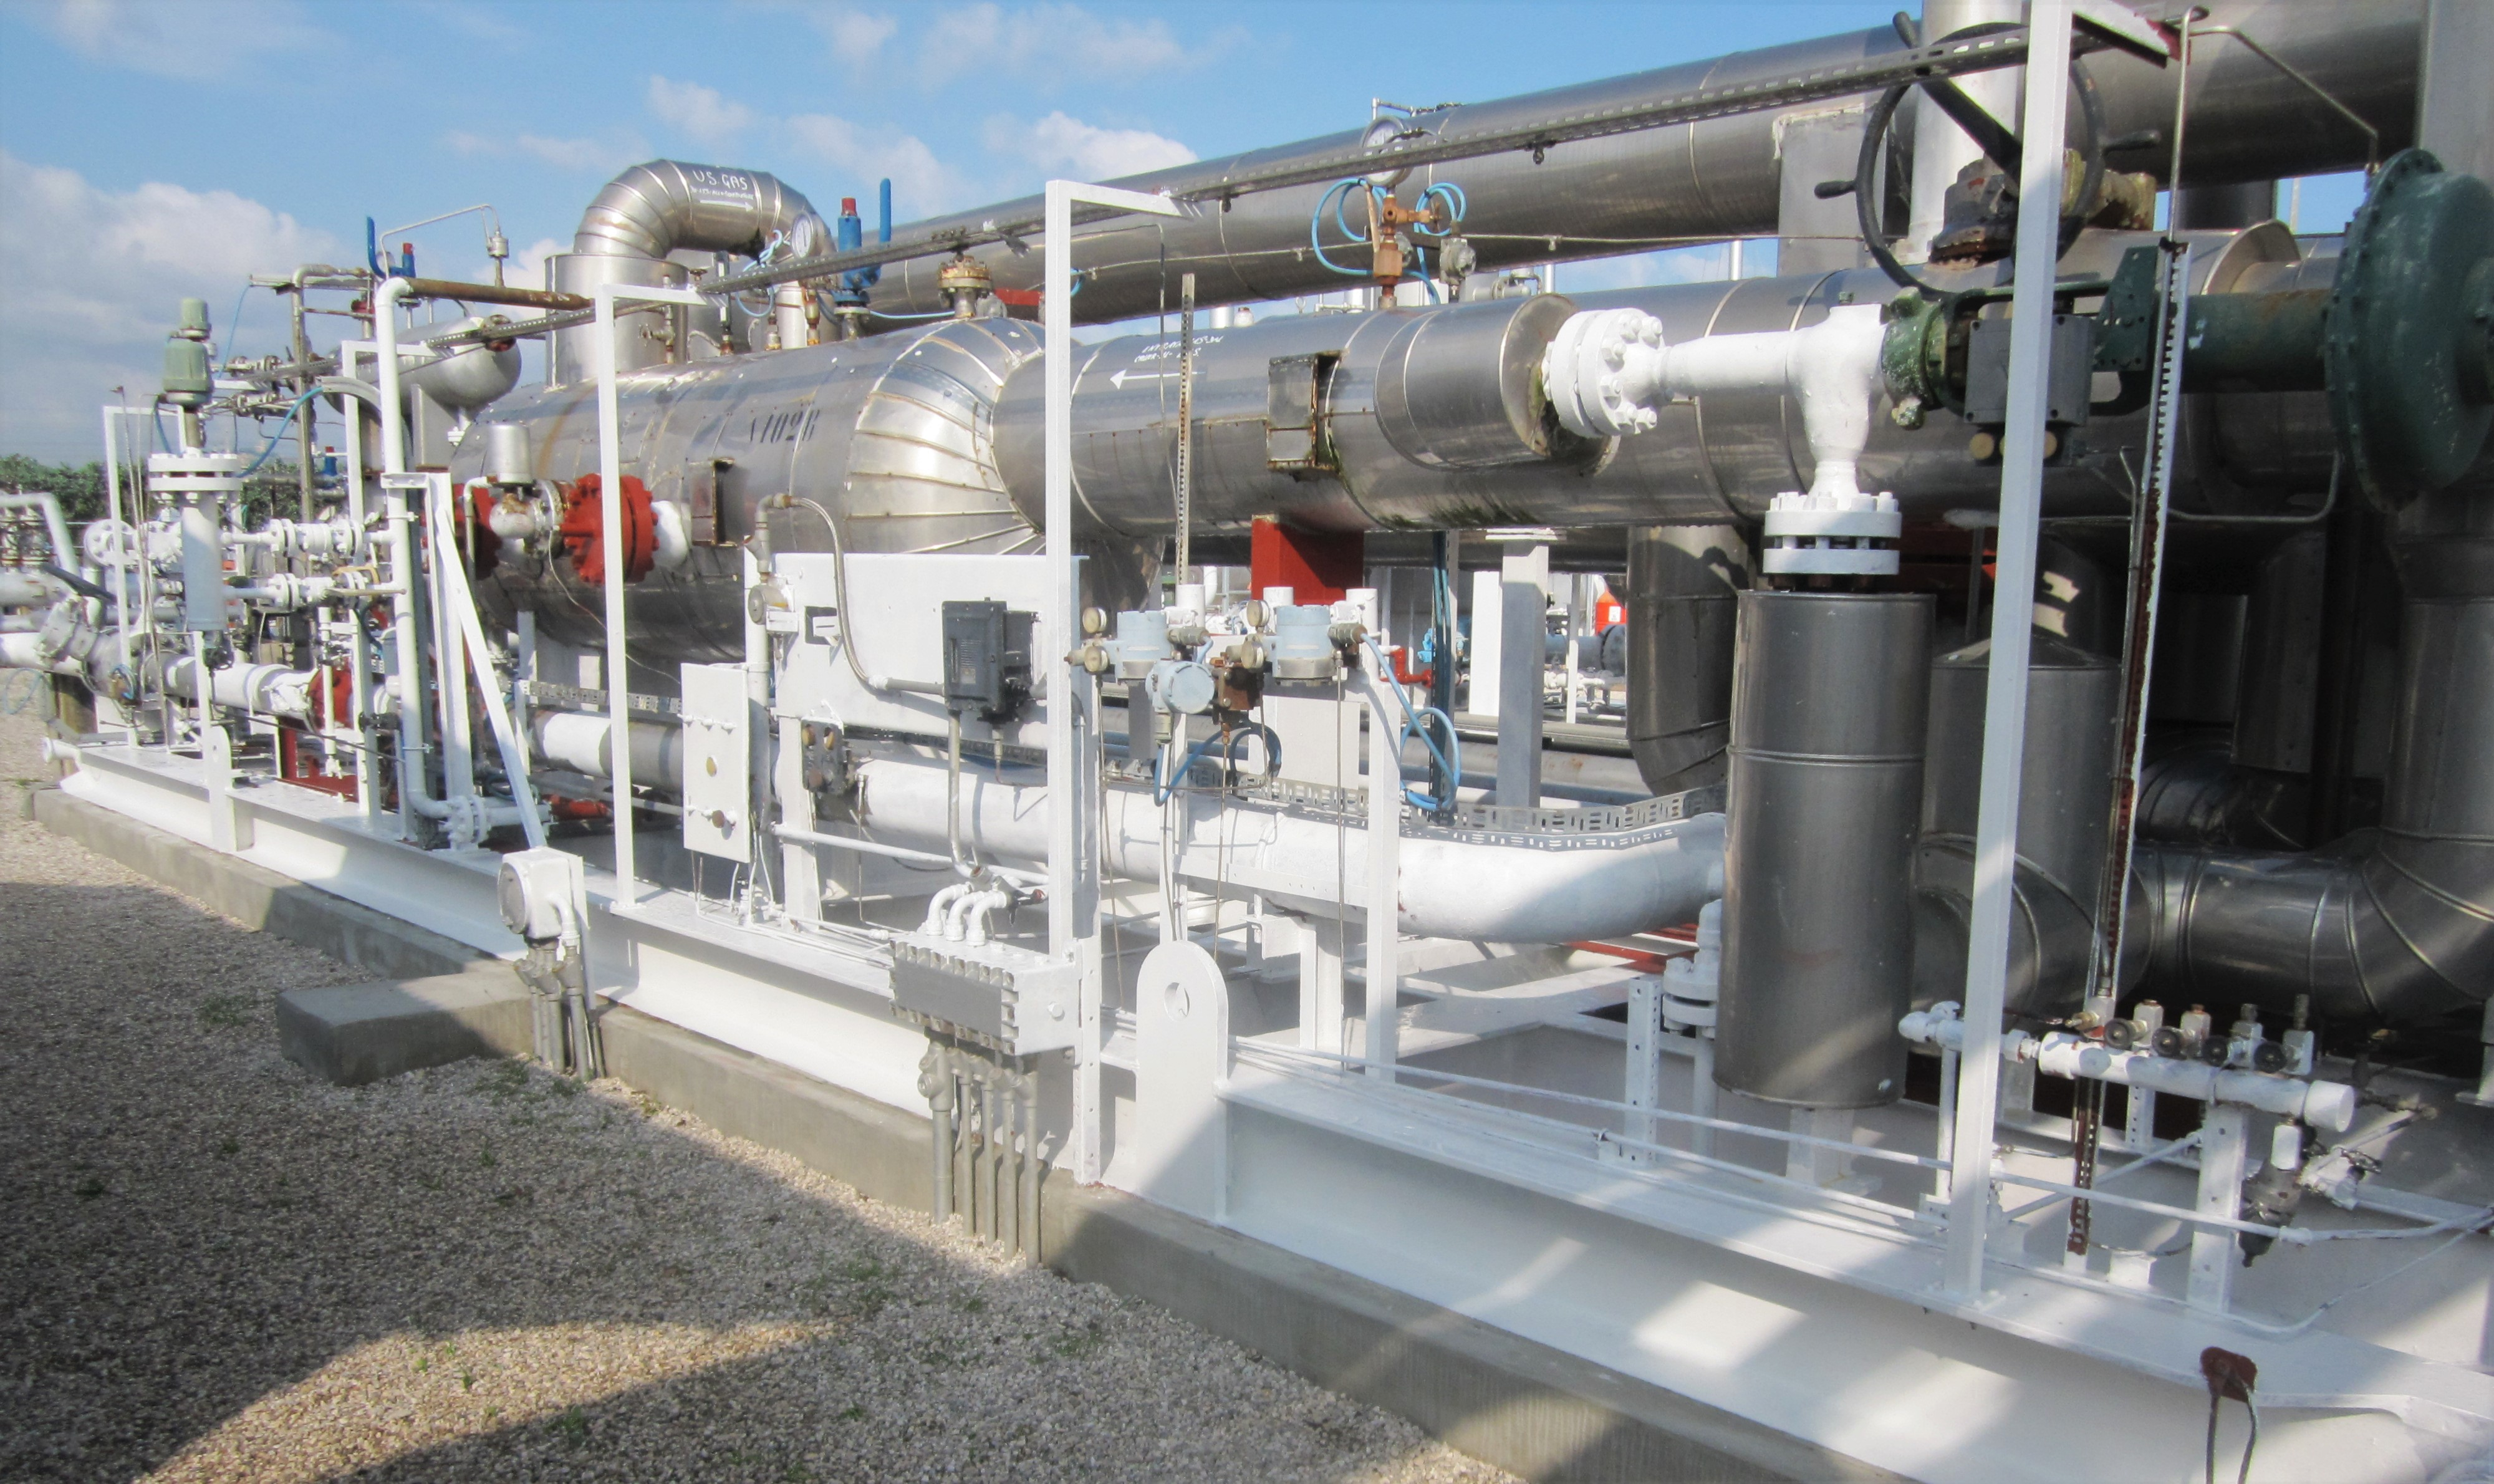
\includegraphics[width=.8\textwidth]{fig/test/centrale/lts.jpg}
    \caption{Separatore a freddo LTS-2.} 
    \label{fig:centrale-lts}
\end{figure}

\subsubsection*{Circuito glicol}
Il glicol dietilenco iniettato nell'unità LTS si carica dell'acqua contenuta nel gas umido. La rigenerazione del glicol viene effettuata nella colonna di distillazione montata in cima al ribollitore.\\
Il glicol idratato penetra nel ribollitore dall'alto della colonna di distillazione, cola lungo la guarnizione controcorrente rispetto al vapore acqueo. Il dispositivo di riscaldamento è costituito da una camera di combustione a forma di U contenente un bruciatore. La temperatura della soluzione glicolata viene controllata da un controllore di temperatura. Il punto di consegna viene fissato dalla riconcentrazione desiderata della soluzione glicolata (120°C). Il glicol riconcentrato cola lungo il troppo pieno nel serbatoio di stoccaggio in cui viene ripreso da una delle pompe di circolazione a scelta. Il livello di glicol nel serbatoio viene controllato da un regolatore di livello. Tale controllore agisce attraverso la valvola a tre vie montata a valle della pompa di circolazione di servizio per mezzo di rubinetterie a punteruolo che devono essere posizionate correttamente. In tal modo, la portata messa in circolo è funzione del consumo richiesto per l'iniezione di glicol nell'unità.\\
Oltre al circuito glicol, la centrale è dotata di sistema metanolo, impiegato per scongelare nell'immediato idrati che si possono generare lungo tutto l'impianto.

\subsubsection*{Riscaldatori}
L'unità di riscaldamento è costituita da scaldatori (\textit{heater}, \figref{fig:scaldatore}) indiretti a bagno d'acqua. La loro potenza è di 780.000 kcal/h (3 MBTU/h) e permette di elevare a 15°C una portata massima di gas di 46.000 m\ap{3}/h.\\
Lo scopo principale del riscaldamento del gas è quello di portare il gas alla temperatura minima richiesta per la sua distribuzione (dettato quindi dalle specifiche), il riscaldamento dei liquidi condensati nell'unita LTS e la rigenerazione del glicol nella colonna di distillazione.\\
Come fonte combustibile viene impiegato del \textit{fuel gas}, il quale viene consumato nella camera di combustione immersa nella parte inferiore del bagno d'acqua. La regolazione della temperatura avviene tramite delle valvole di regolazione termica (\textit{temperature control valve}, TCV) che inviano più o meno gas ai due bruciatori in funzione della temperatura del gas in uscita e della consegna fissata.

\begin{figure}[htbp] %%% Immagine pompa dosatrice
    \centering
    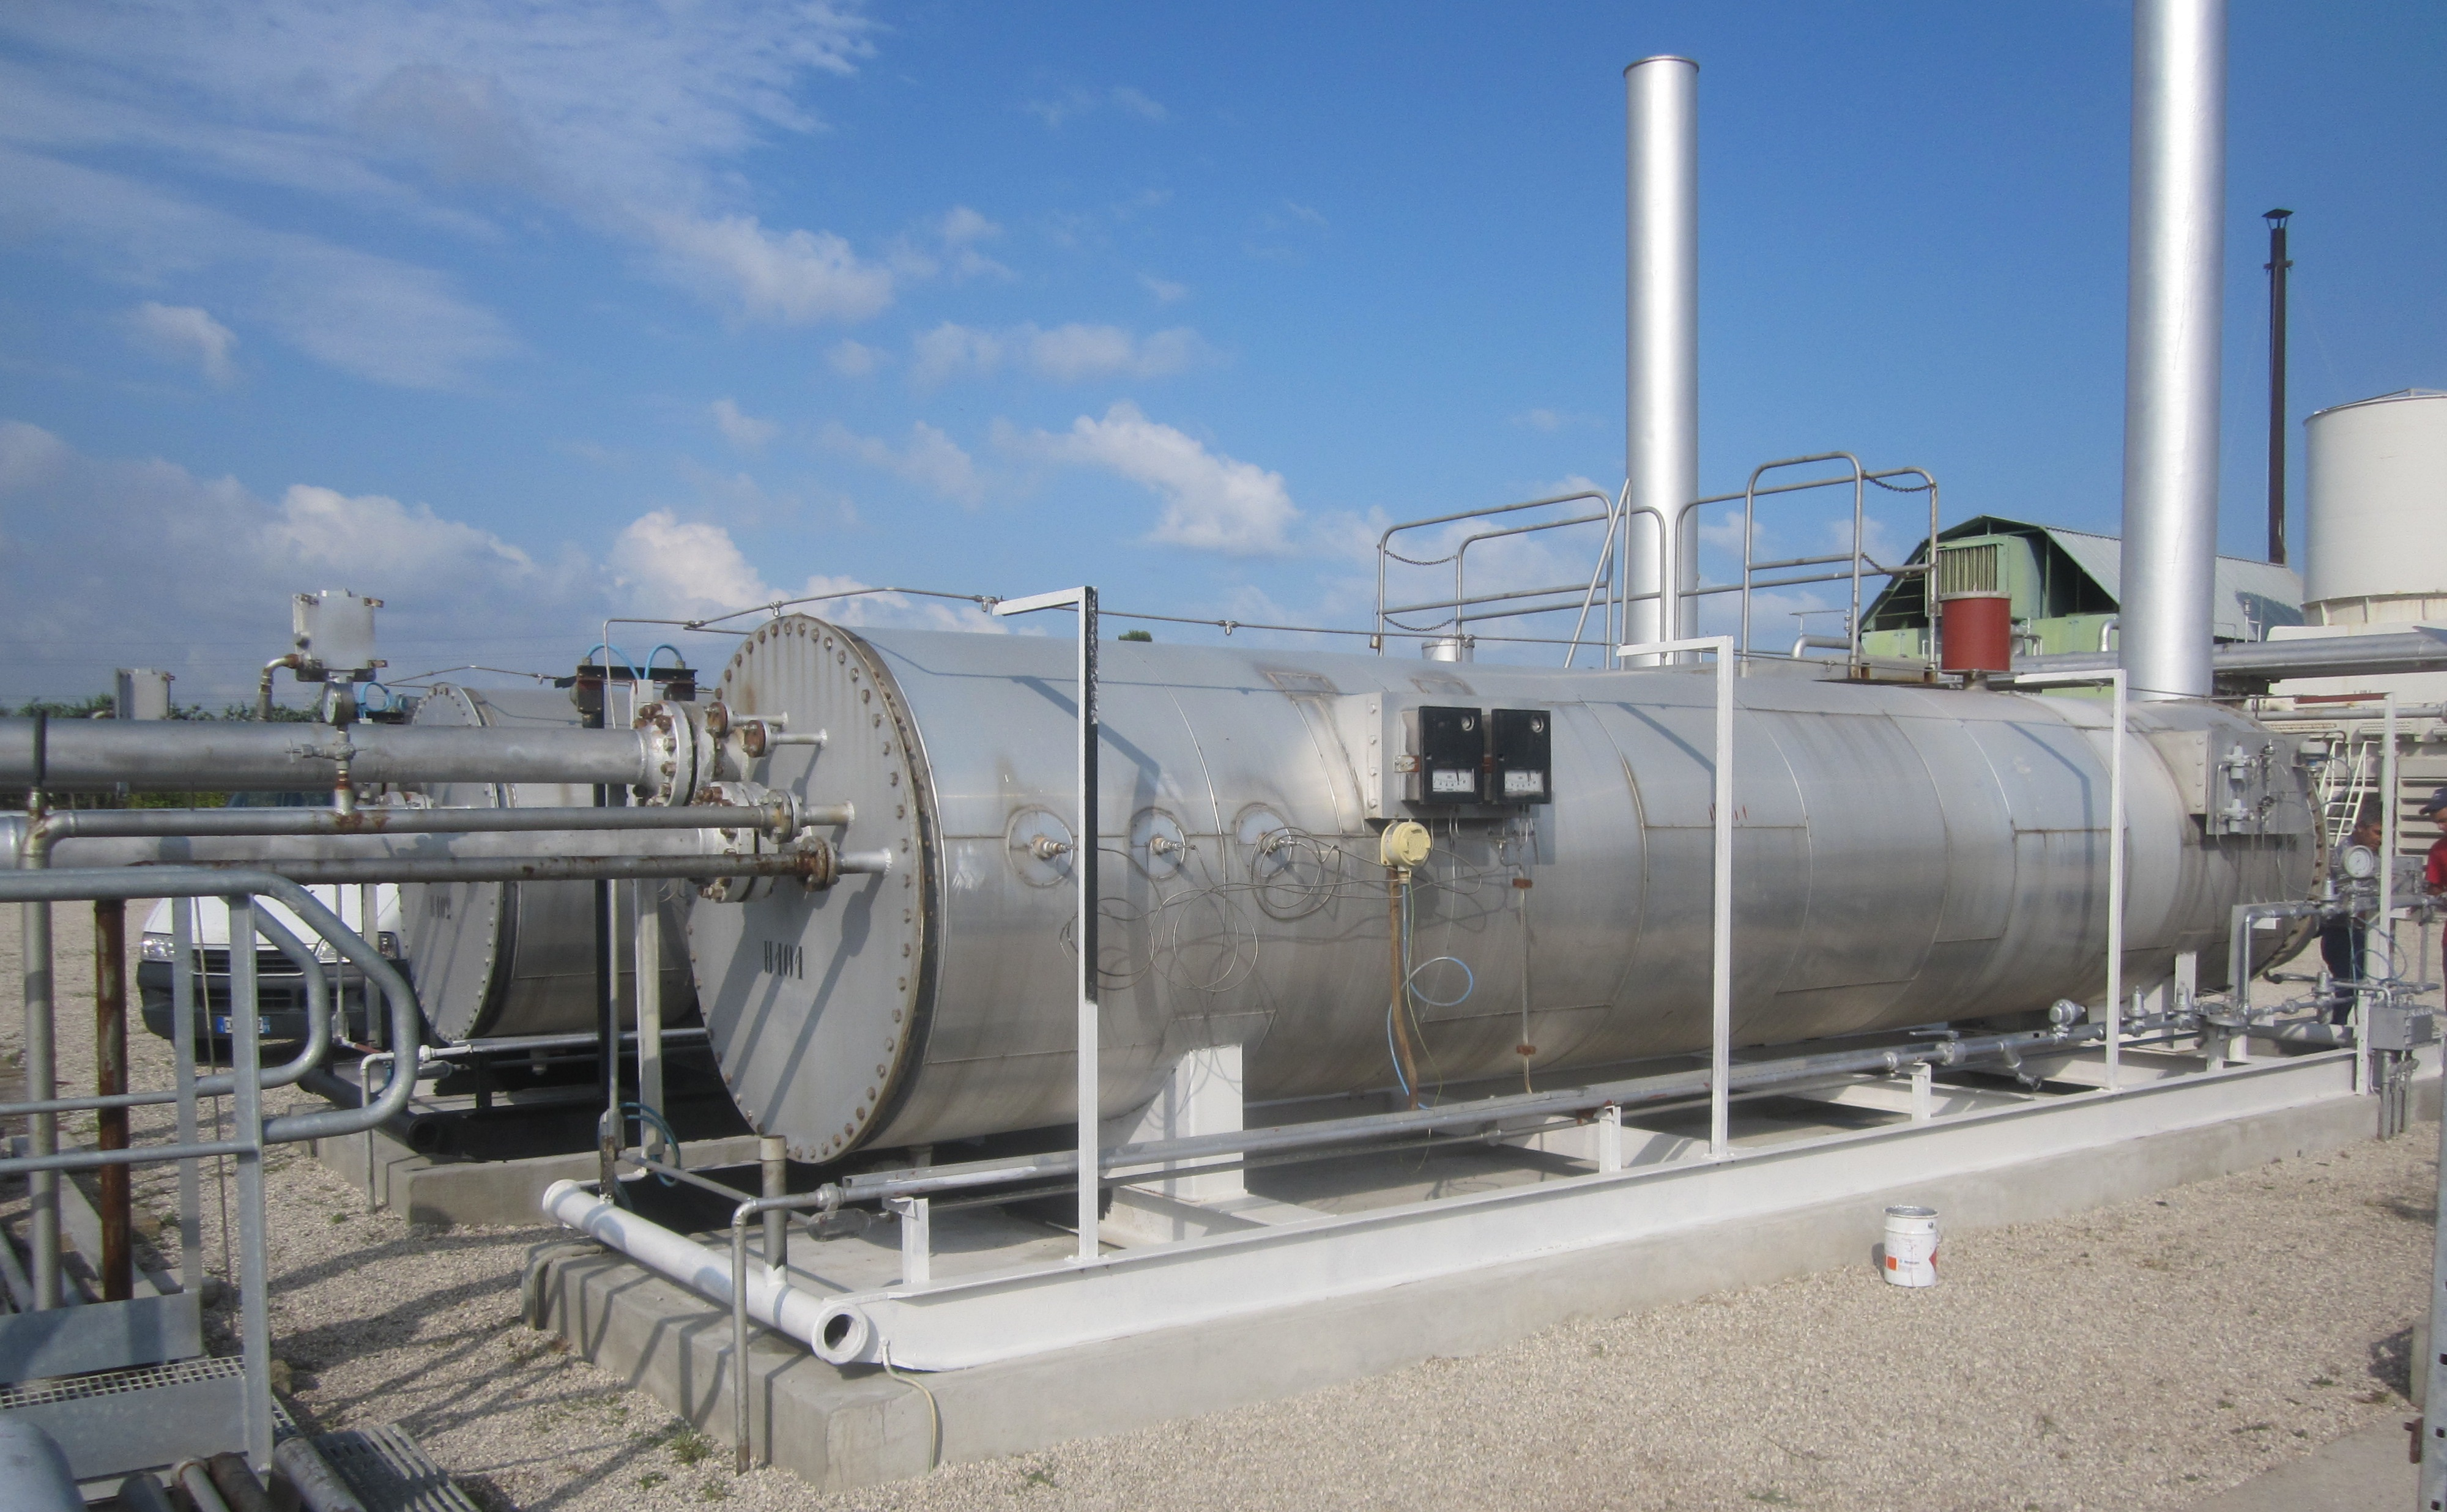
\includegraphics[width=.7\textwidth]{fig/test/centrale/scaldatore}
    \caption{Scaldatore indiretto a bagno d'acqua.} 
    \label{fig:scaldatore}
\end{figure}

\subsubsection*{Filtri}
Il gas dopo il riscaldamento viene filtrato tramite due filtri a cartucce Castagnetti 311 collocati in parallelo. I filtri sono installati al fine di abbattere ulteriori residui (acqua o condensati) prima dell'immissione del prodotto in rete nazionale.

%\subsubsection{Sicurezza}
%\paragraph{Sicurezza degli impianti di processo}
%\paragraph{Sicurezza detenzione gas}
%\paragraph{Rilevazione incendio}
%\paragraph{Sistema antincendio}

\subsubsection*{Rete elettrica}
L'energia elettrica arriva in centrale alla tensione di 10 kV e viene convogliata al quadro a media tensione (QMT-1), previsto per una tensione nominale di 10/20 kV, 50 Hz in sistema trifase a neutro isolato. Il quadro è costituito da un arrivo e due partenze, da cui sono alimentati due trasformatori da 800 kVA, i quali convertono la tensione a 380 V. La corrente passa infine dai trasformatori al quadro a bassa tensione tramite cavo unipolare. Per l'alimentazione degli ausiliari è previsto un raddrizzatore con relativa batteria di accumulatori. L'impianto luce è collegato con un trasformatore a monte da 30 kVA che converte la tensione da 380 V a 220 V.

\subsubsection*{Rete aria}
L'aria strumenti consente il controllo delle valvole dislocate in centrale tramite una rete pneumatica ad aria. La compressione dell'aria è a opera di due compressori a vite, a iniezione di olio, monostadio, raffreddato ad aria e azionato da motore elettrico tramite cinghia dentata.\\
Nella reta pneumatica l'aria viene aspirata tramite un filtro, passa nell'elemento compressore dove viene compressa. L'aria compressa e l'olio passano, tramite una valvola di ritegno, nel serbatoio aria/separatore olio, dove il lubrificante viene separato dalla miscela aria-olio. L'aria compressa viene scaricata attraverso un rubinetto di uscita dopo aver attraversato una valvola di alta pressione (PSH, \textit{Pressure Safety High}), un refrigeratore dell'aria e uno scaricatore di condensa.\\
La pressione dell'aria forza l'olio dal serbatoio dell'aria, attraverso il refrigeratore dell'olio, il filtro, il limatore e la valvola di arresto dell'olio, fino all'elemento compressore e ai punti di lubrificazione.

\subsubsection*{Strumentazione di misura e di conteggio presente sul campo}
A monte di ogni separatore è installato un misuratore venturimetrico e le misure istantanee di pressione differenziale, pressione e temperatura sono garantite dai trasmettitori elettronici al calcolatore (VESCOM 3V) il quale provvede ad effettuare il calcolo della portata e il conteggio fiscale. Misuratori venturimetrici associati ai calcolatori e/o registratori analogici (Triplex) sono presenti anche in ogni area produttiva collegata alla centrale di trattamento. La telelettura da remoto dei \textit{flow computer} esterni alla centrale avviene attraverso un modem GSM esterno.
\begin{figure}[htbp]
    \centering
    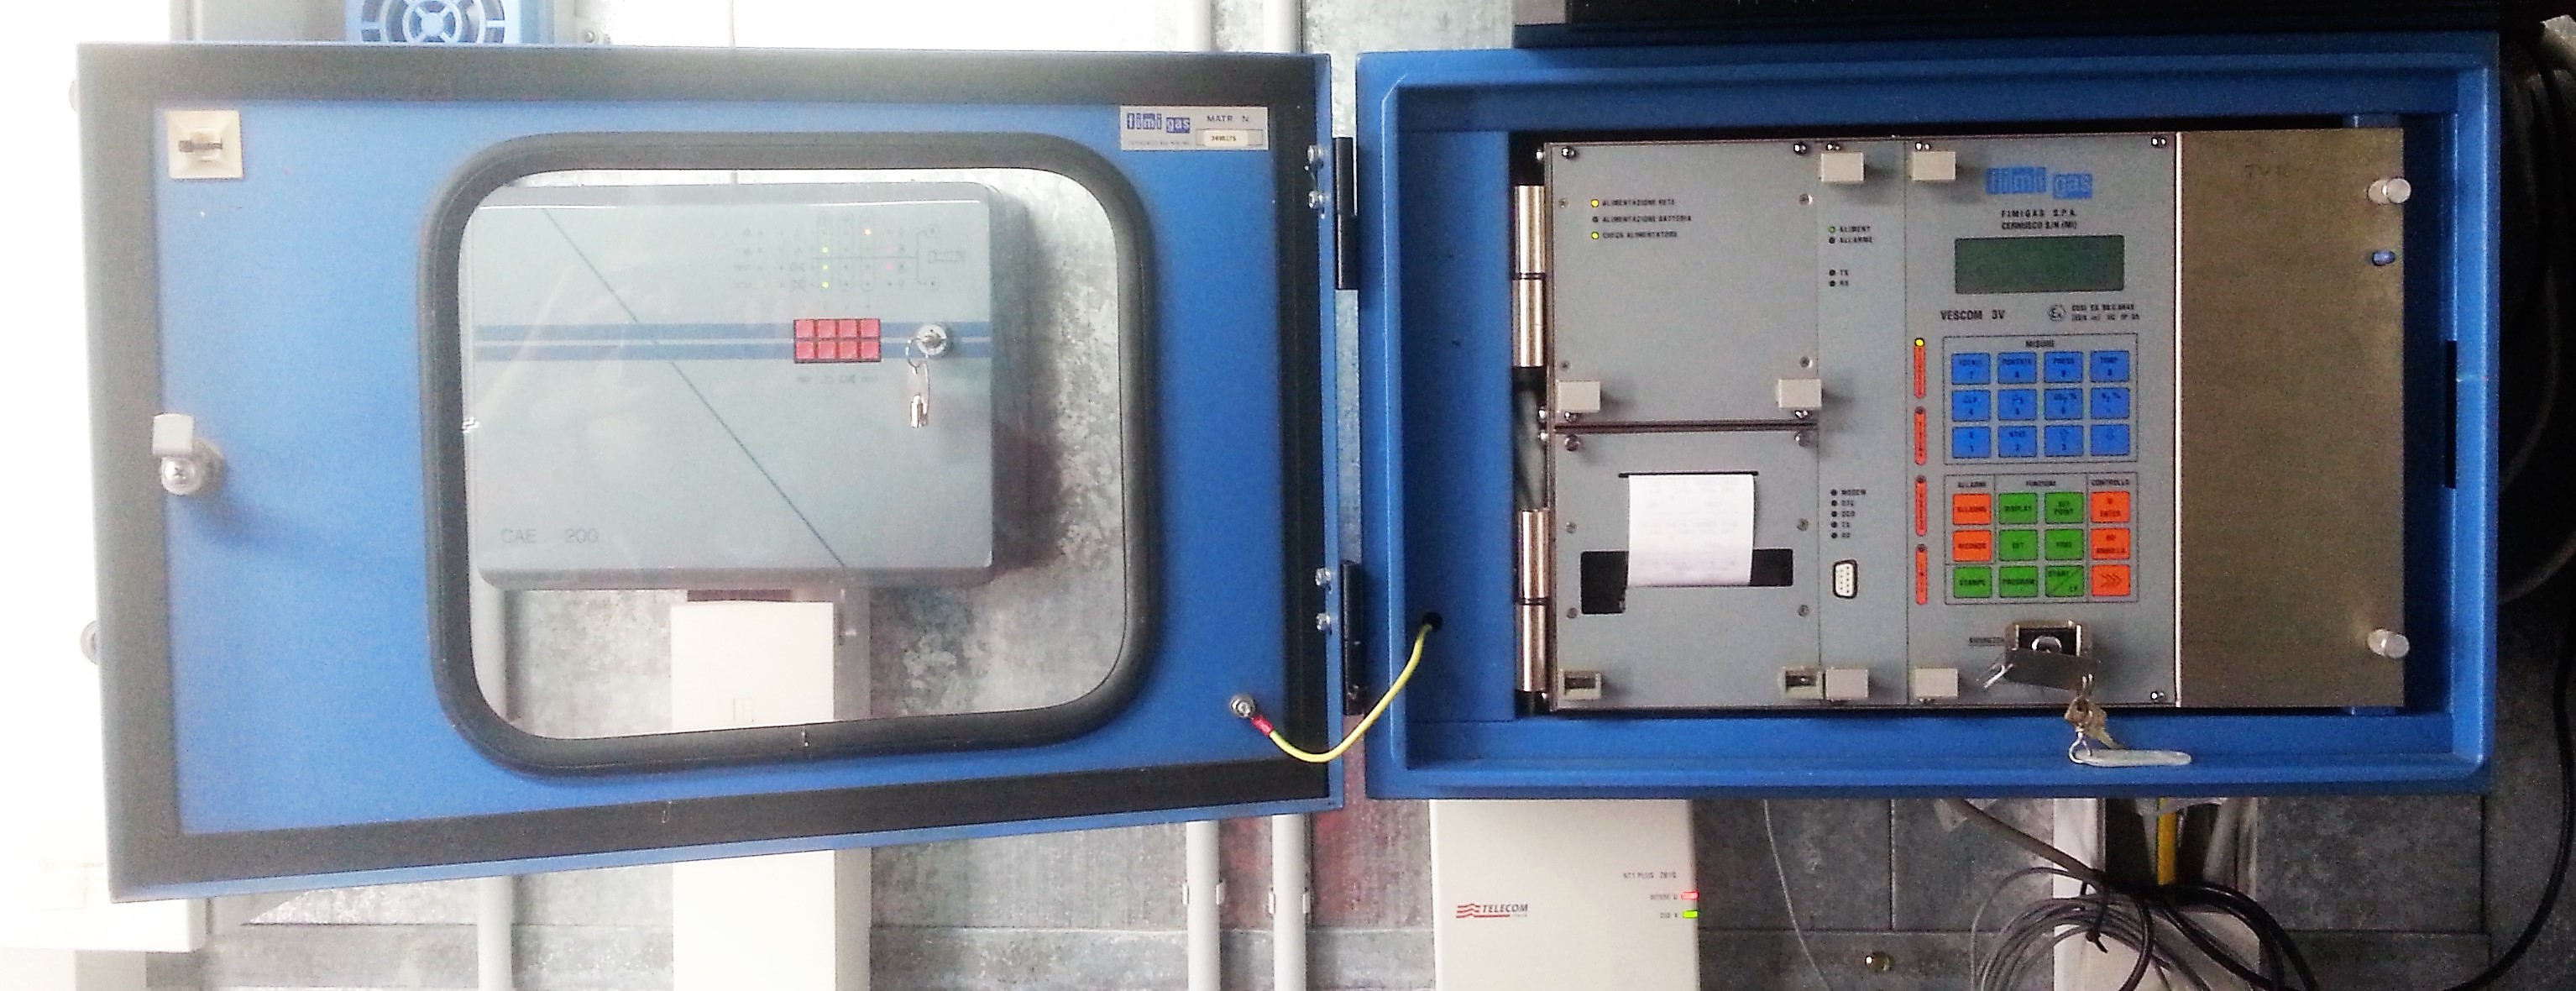
\includegraphics[width=\textwidth]{fig/test/vescom}  
	\caption{Unità VESCOM 3V.}
	\label{fig:vescom}
\end{figure}
Il calcolo dei volumi d'acqua associati alla produzione di gas naturale è legato alla modalità di scarico dei liquidi nei separatori.\\
Sul campo di San Marco, ogni pozzo è dotato di separatore proprio e lo scarico in vasca avviene tramite interruttori di livello. L'attivazione di questi dispositivi avviene una volta raggiunto un determinato battente idrostatico, la valvola di scarico si attiva e l'acqua defluisce nelle vasche di stoccaggio. L'interruttore di livello è associato a un contatore, il quale registra il numero di attivazioni della valvola di scarico. L'acqua di produzione confluisce in un'unica vasca di stoccaggio e si verifica giornalmente la quantità totale misurando l'innalzamento del livello. Il volume d'acqua calcolato viene così ripartito su ogni separatore in proporzione agli scatti giornalieri registrati dal contatore.\\
I separatori in centrale S101, S112 e S111 sono dotati invece di regolatori di livello, i quali mantengono costante il battente idrostatico all'interno della camera. In questo caso la misura dell'acqua prodotta avviene tramite lettura dell'innalzamento giornaliero dei serbatoi S113, S114 e S117 dedicati allo stoccaggio e smistamento dell'acqua di processo.

\begin{figure}[htbp]
    \centering
    \subfloat[][Vista frontale del separatore.]
    {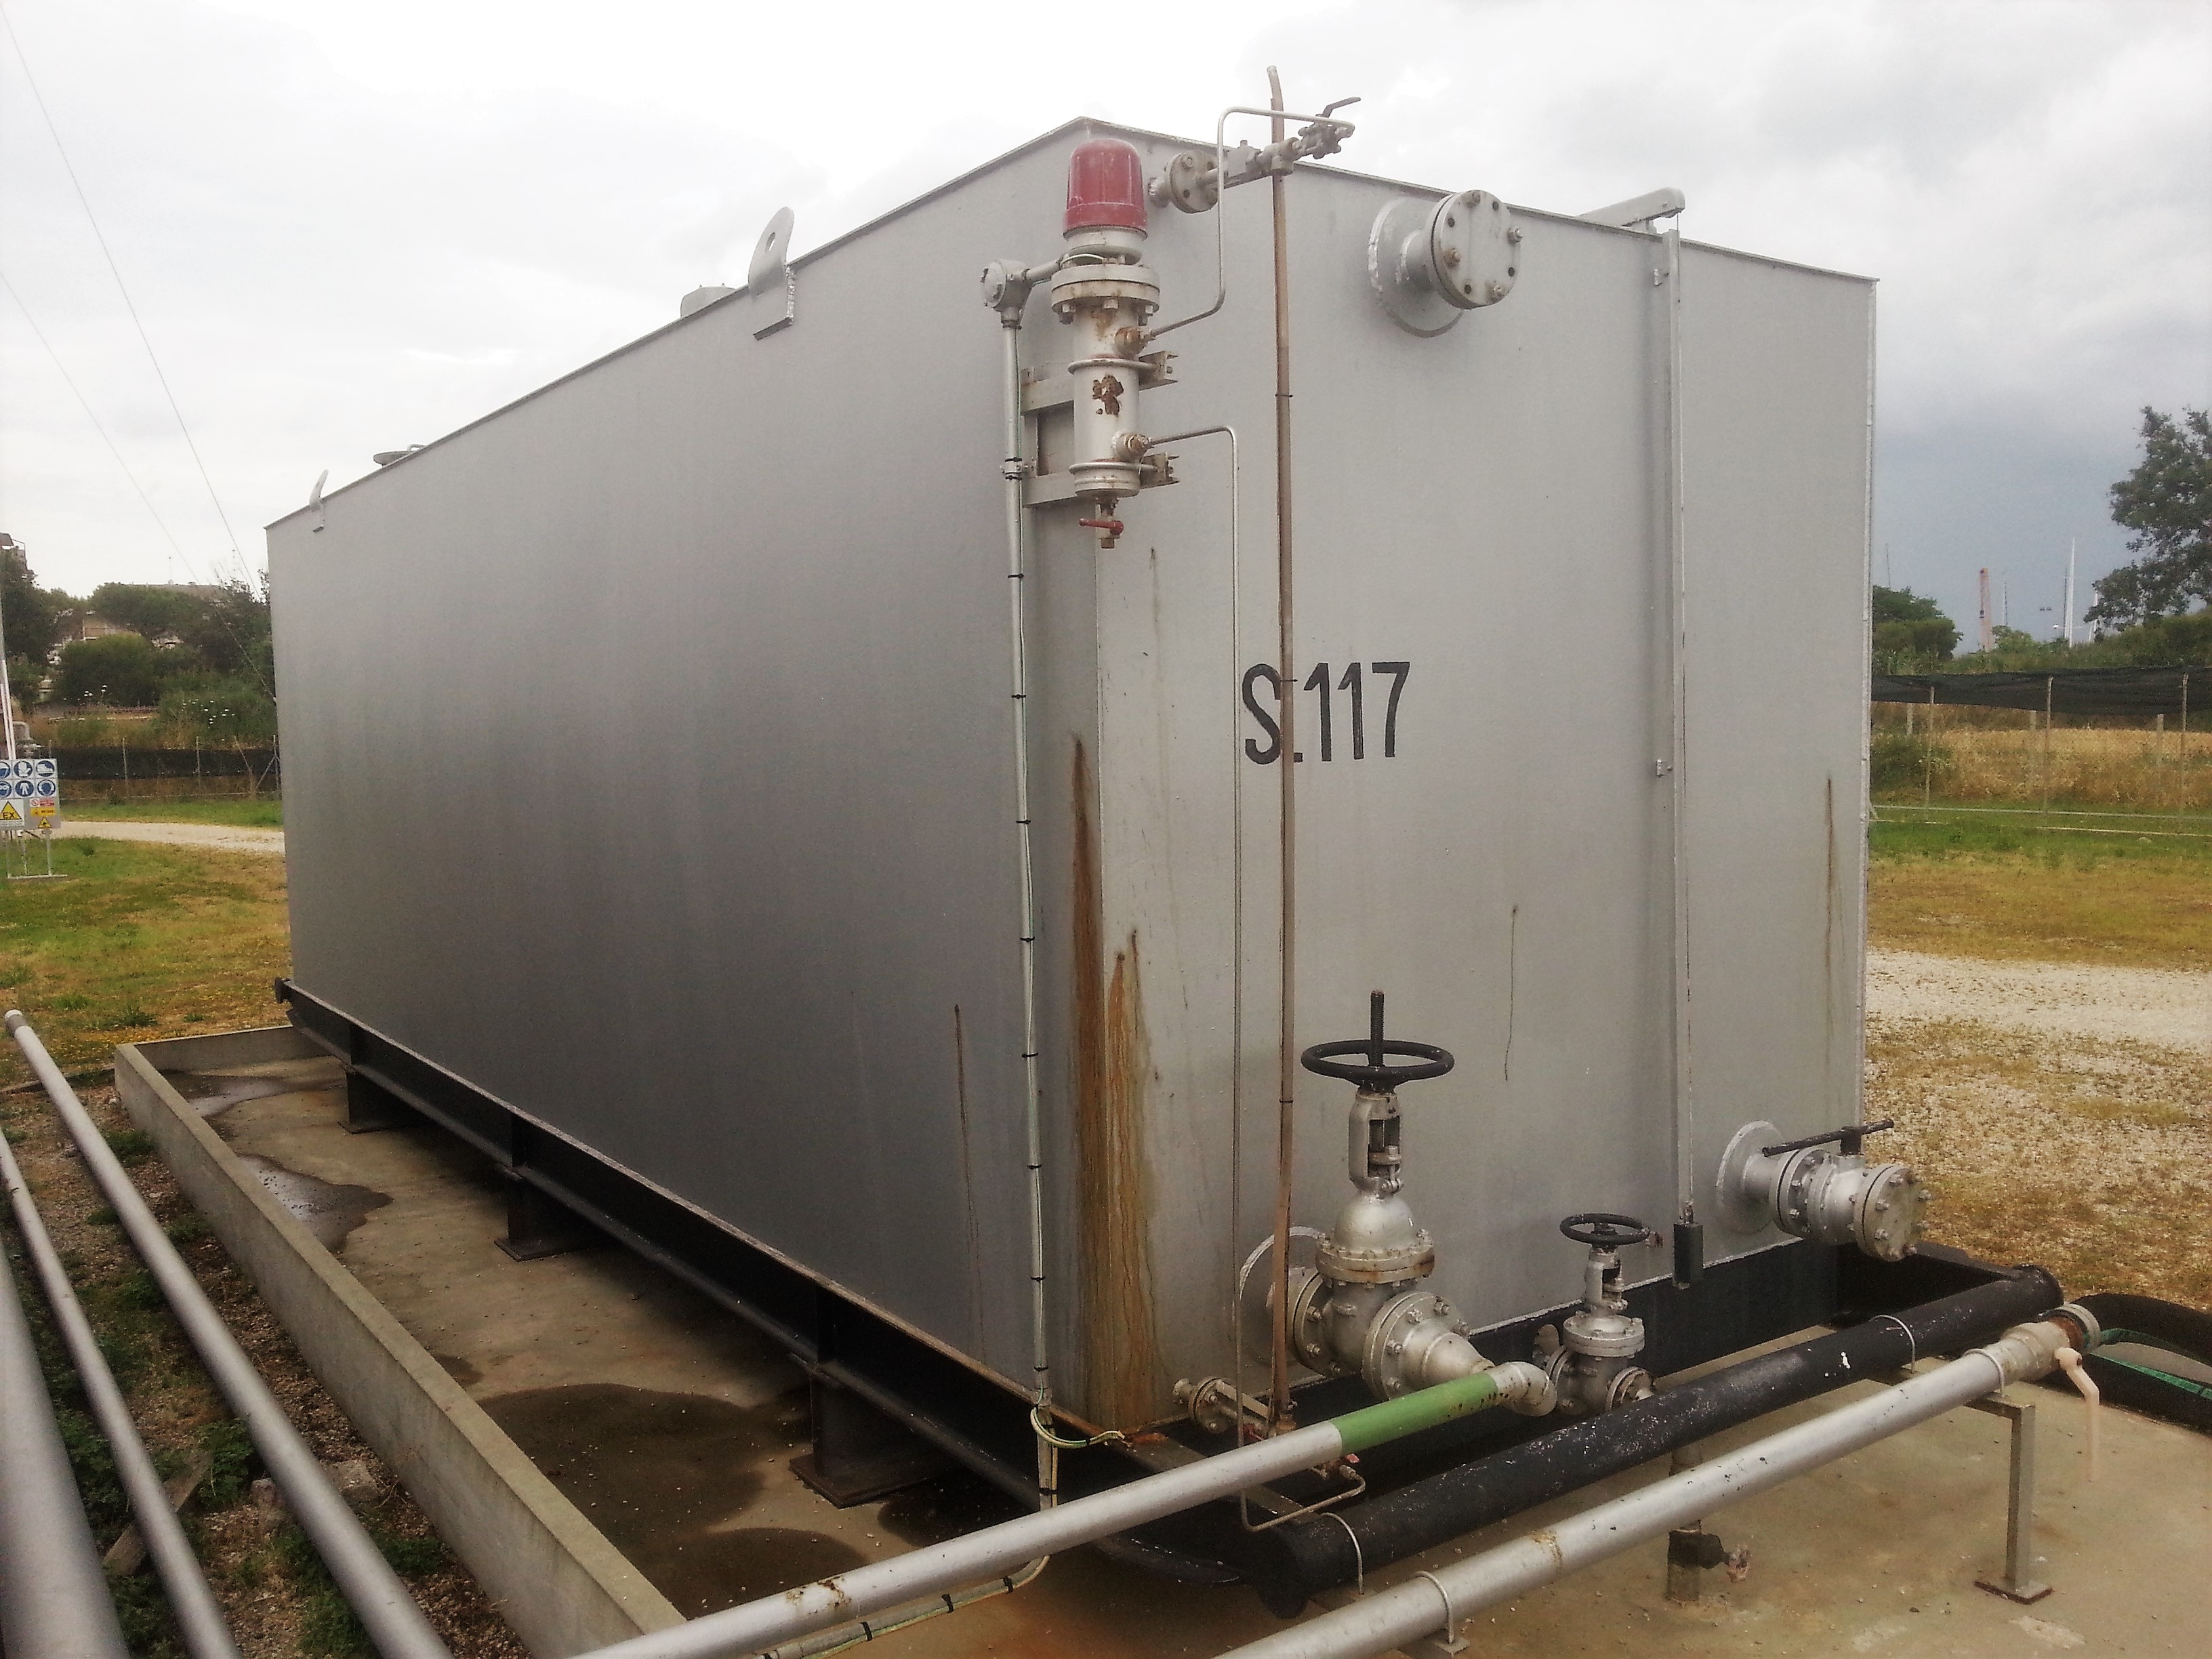
\includegraphics[height=.25\textheight]{fig/test/acque1}  \label{fig:acque1}} \qquad
    \subfloat[][Dettaglio del misuratore del battente idrostatico.]
    {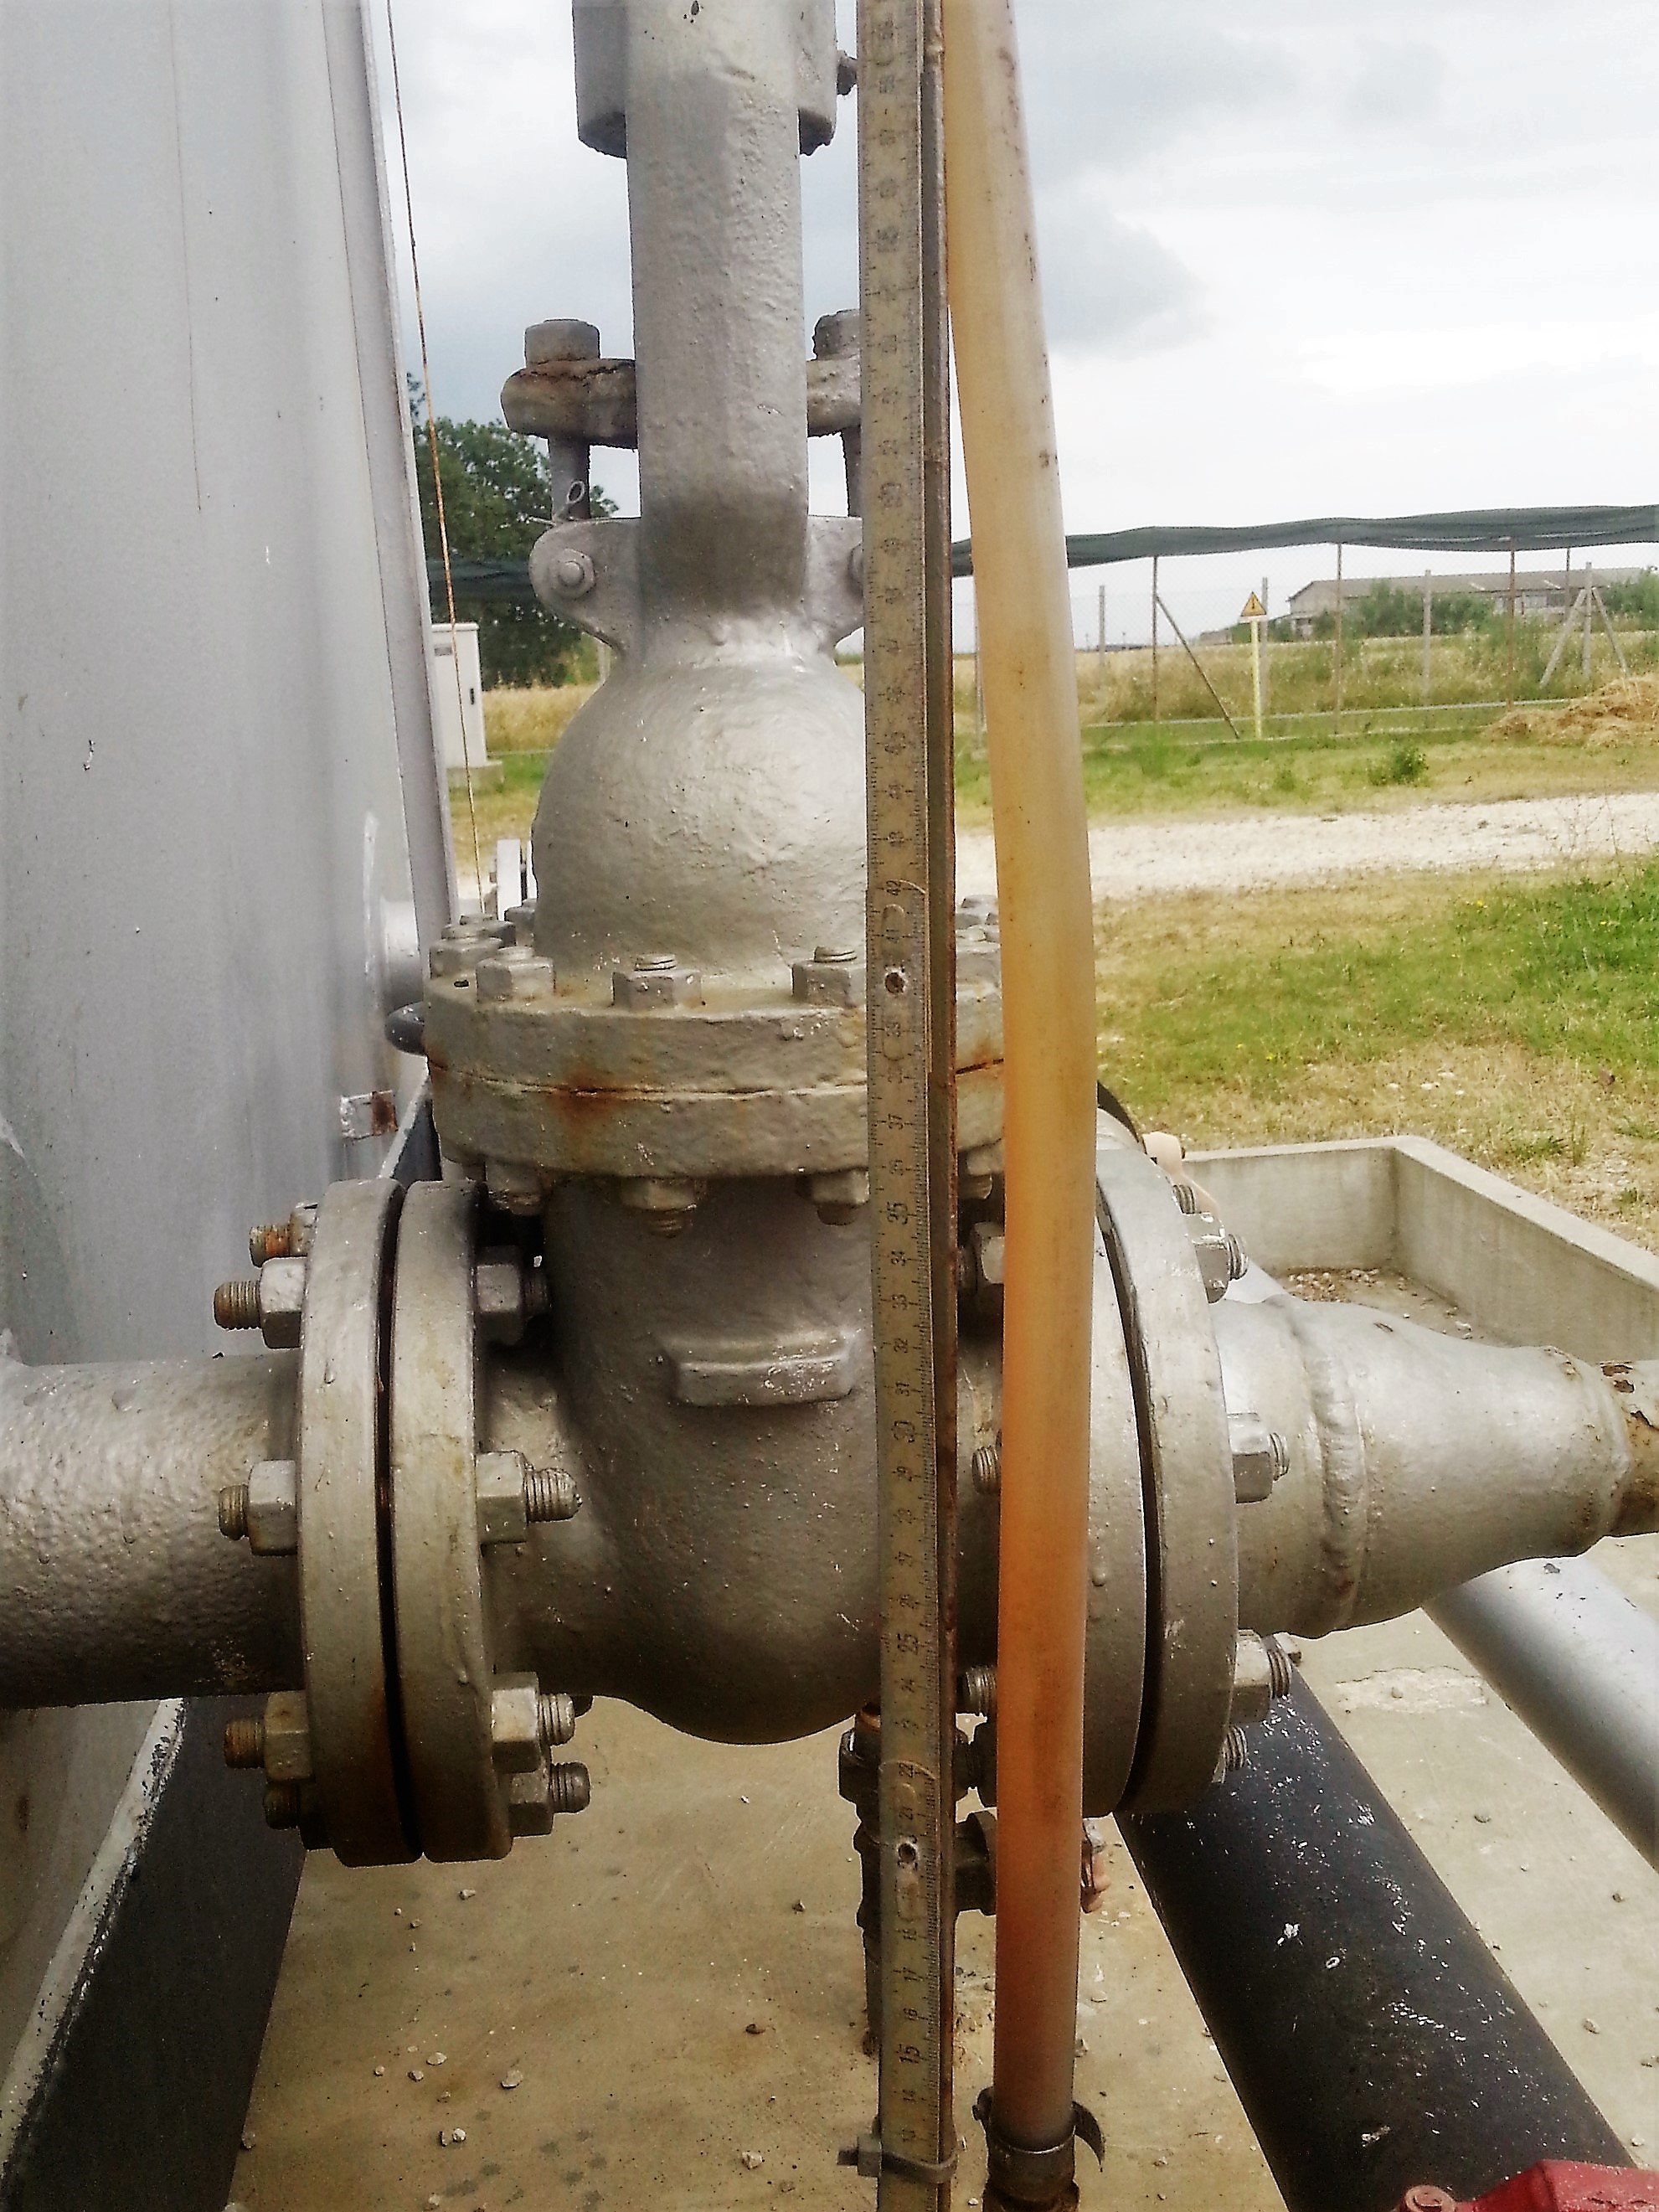
\includegraphics[height=.25\textheight]{fig/test/acque2} \label{fig:acque2}} 
\caption{Serbatoio di stoccaggio acque S117.}
\label{fig:acque}
\end{figure}

%-------------------------------------------------------------------

\section{Configurazione sperimentale: materiali e modalità di esecuzione}
\sectionmark{Configurazione sperimentale}
Il giorno venerdì 12 giugno 2015 è stato effettuato il test di campo nell'area produttiva di San Marco con la collaborazione della Chimec S.p.A.. Tra il 23 e il 27 febbraio 2015 c'è stata una precedente applicazione di schiumogeno in campo, che ha però riguardato la deliquificazione del pozzo Cozza, attualmente fermo e attivato periodicamente una volta ristabilita la pressione massima a fondo pozzo.\\

\subsection{Schiumogeno}
Il prodotto Phoenix 6163 è uno schiumogeno prodotto dalla Chimec S.p.A.. Disciolto in acqua, fa diminuire notevolmente la tensione interfacciale che compete alla superficie di separazione fra la soluzione diluita così ottenuta e la fase gassosa. Dal punto di vista chimico lo schiumogeno consiste in una miscela di alchilpoliglicoletere, surfactante non ionico, in alcol. \\
Lo schiumogeno ha effetto in soluzione acquosa con concentrazioni pari o superiori ai 5000 ppm. Il prodotto non comporta variazioni sostanziali ai parametri chimico-fisici dell'acqua di produzione, che può quindi essere convogliata ai pozzi iniettori senza trattamenti preliminari.\\ 
Il \textit{foamer} è distribuito e stoccato in contenitori IBC da 1000 litri.
\subsection{Antischiuma}
Il prodotto CHIMEC Phoenix 8161 è un antischiuma sempre prodotto dalla Chimec S.p.A.. \'E una miscela di derivati non ionici e surfactanti in soluzione acquosa. La sua azione consente di abbattere la schiuma all'interno dei separatori della centrale SGM. \\
Il defoamer agisce sulla soluzione schiumosa per concentrazioni pari o superiori ai 5000 ppm. L'uso del prodotto non preclude l'immissione delle acque di produzione nei pozzi iniettori senza eventuali trattamenti.\\
Anche il \textit{defoamer} è distribuito e stoccato in contenitori IBC da 1000 litri.
\begin{table}[htbp]
\centering
\footnotesize
\caption{Parametri fisico-chimici dello schiumogeno e dell'antischiumogeno presi dalle rispettive schede di sicurezza.}
\label{tab:schedasicurezza}
\begin{tabular}{|p{.4\textwidth}|p{.3\textwidth}p{.3\textwidth}|}
\hline
{\bf Parametri}                & {\bf CHIMEC Phoenix 6163} & {\bf CHIMEC Phoenix 8161} \\ \hline \hline
\textbf{Stato fisico a 20°C }           & Liquido                                       & Liquido                                       \\\hline
\textbf{Colore  }                       & Da trasparente a giallo chiaro                & Da trasparente a opalescente                  \\\hline
\textbf{Punto di congelamento (°C) }    & n.d.                                          & n.d.                                          \\\hline
\textbf{Punto di ebollizione (°C)  }    & c.a. 140                                      & c.a. 100                                      \\\hline
\textbf{Punto di scorrimento (°C) }     & n.d.                                          & \textless0                                    \\\hline
\textbf{Densità a 20°C (gr/cm\ap{3}) }  & 0,96\(\pm\)0.02                               & 0,99\(\pm\)0,02                                   \\\hline
\textbf{Viscosità a 20°C (cP) }         & \textless100                                  & \textless100                                  \\\hline
\textbf{Solubilità in acqua (\% peso)}  & Totalmente solubile                           & Parzialmente solubile                         \\\hline
\textbf{Mezzi solventi  }               & Acqua                                         & Acqua                                         \\\hline
\textbf{pH in acqua distillata }        & (1\%) c.a. 6,0                                & 7,0\(\pm\)1,0                                     \\\hline
\textbf{Punto di infiammabilità   }     & c.a. 19                                       & n.d.                                         \\
\hline
\end{tabular}
\end{table}


\subsection{Punto di iniezione}
L'iniezione in batch e in continuo del \textit{foamer} è attuata sulla linea di mandata del campo San Marco (\figref{fig:mandata}). Inizialmente l'iniezione in-batch è stata pensata in una linea ausiliaria appartenente all'impianto di trattamento in quiescenza presente a San Marco. L'ipotesi è rigettata poiché il \textit{bypass} è collocato a troppa distanza dalla linea di mandata. Lunghe distanze all'interno dell'area possono tradursi in maggiori perdite di carico, inibendo in parte l'azione di "shock" provocata dal batch. Inoltre si è ritenuto che il tratto iniziale potesse essere stato interessato da acqua stagnante (il tratto è completamente orizzontale), condizione sfavorevole all'azione ottimale del \textit{foamer}.
A monte della linea di mandata è presente una valvola a sfera e subito dopo l'apparato di misura composto da tubo venturimetrico e rilevatori di pressione assoluta e temperatura. L'unità è collegata sia al VESCOM 3V per il calcolo istantaneo, orario e giornaliero della portata di gas e al registratore analogico Triplex. Di seguito si collocano delle valvole dedicate all'installazione di manometri di misura e di controllo e una PCV. Più avanti sono locate due PSV di scarico (\textit{blowdown valve}), un'altra valvola di misura della pressione, un'altra valvola a sfera, una valvola di arresto di sicurezza (\textit{Shut-Down Valve}, SDV) e due valvole rispettivamente di alta (\textit{Pressure Safety High}, PSH) e bassa pressione (\textit{Pressure Safety Low}, PSL).\\
La linea di mandata è stata isolata tramite le valvole a sfera presenti. L'immissione di schiumogeno avvenuta tramite la rimozione temporanea dei dispositivi di lettura e controllo della pressione, in particolare dei manometri presenti a monte della PCV per l'applicazione in-batch e del manometro a monte della SDV, associata al quadro di controllo generale, per l'immissione in continuo.

\begin{figure}[htbp] %Immagine layout di mandata
    \centering
    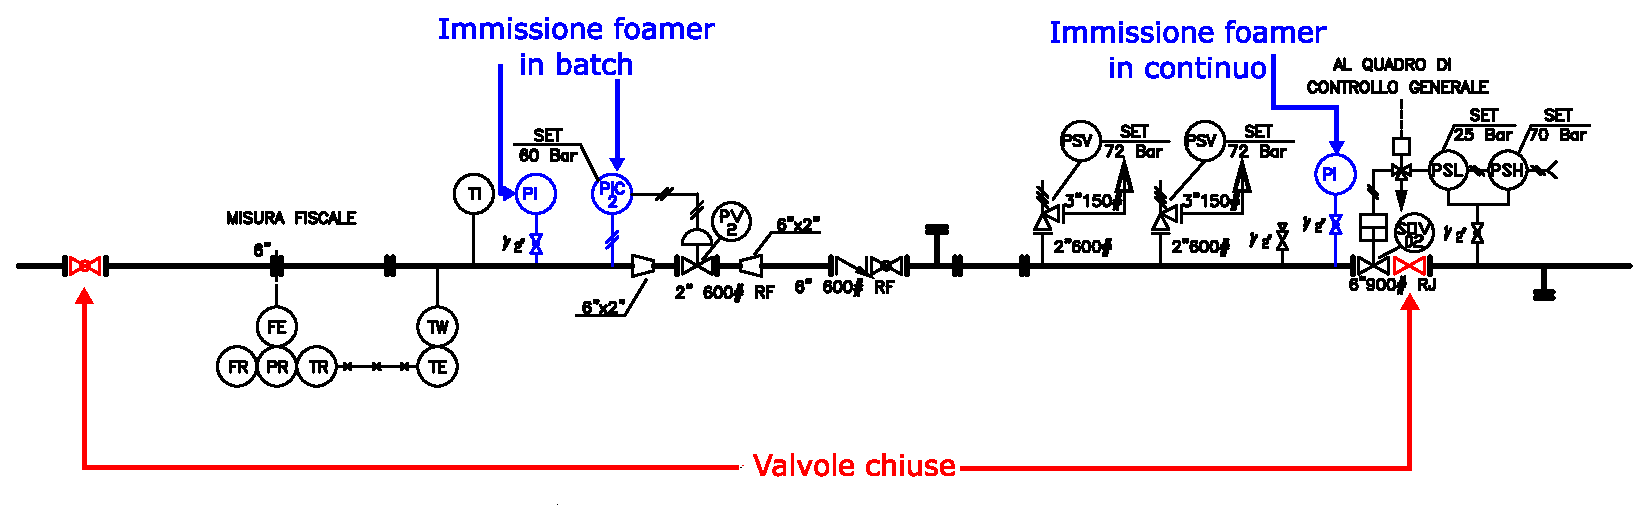
\includegraphics[width=\textwidth]{fig/test/mandata.eps}
    \caption{Layout linea di mandata SNM, modalità di applicazione del batch.} 
    \label{fig:mandata}
\end{figure}

\subsection{Iniezione in-batch}
Scartata l'ipotesi della linea ausiliaria, si è deciso per il blocco temporaneo della produzione tramite iniezione in linea.\\
Per l'applicazione in-batch si è deciso di introdurre una quantità di schiumogeno che generasse uno shock consistente, in modo da attivarsi nell'immediato e favorire così l'applicazione dello schiumogeno in continuo.\\
Come volume d'acqua stimato \(\hat{V_{w}}\) all'interno in condotta è stato preso il valore dell'acqua spiazzata nell'ultimo piggaggio effettuato il 30 luglio 2013: lo scovolo per l'occasione spiazzò 14,5 m\ap{3} di acqua dalla condotta.\\
Conoscendo la concentrazione \(c_f\)=5000 ppm di attivazione dello schiumogeno, si è calcolata il volume minimo \(V_{f,min}\) richiesto in condotta:
\[V_{f,min}= c_f\,\hat{V_w}=0,0725 \, \mathrm{m^3}=72,5 \, \mathrm{l} \label{eq:volfoamer}\]
Non conoscendo perfettamente i volumi di acqua in condotta e non avendo mai applicato degli schiumogeni in orizzontale, il valore precedentemente calcolato è stato preso come semplice riferimento e si è optato in prima fase per un volume sovrastimato \(\hat{V_{f}}\) di 100 litri.\\
Nello studio preliminare si è scelto anche di introdurre dell'acqua assieme allo schiumogeno, al fine di diminuire la viscosità del prodotto (c.a. 100 cP) e velocizzare l'arrivo del batch al primo avvallamento. La scelta di acqua come \textit{chaser} deriva dall'applicazione di schiumogeni per pozzi orizzontali, in cui però si fa riferimento a un cuscino di \textit{brine} dal peso specifico superiore all'acqua di fondo pozzo. La quantità di acqua stabilita è di 50 l circa, rispettando il rapporto 2:1 con il prodotto.\\
Per l'immissione di \textit{foamer} sono state chiuse le due valvole a sfera manuali a monte e a valle della linea di mandata. Il tratto interessato è stato depressurizzato tramite l'apertura di una valvola di misura a valle delle PCV.\\
Nel frattempo sono stati preparati i volumi di schiumogeno e acqua precedentemente concordati. I liquidi sono stati raccolti e portati in linea tramite recipienti di 30 l e 50 l. \\
Una volta completata la depressurizzazione si è introdotto il batch in linea (\figref{fig:test-batch-immissione}). Nella condotta sono stati introdotti 40 l di acqua ma solamente 60 l di schiumogeno: il prodotto infatti tracimava dal punto di iniezione ed è stato impossibile continuare l'applicazione.\\
Se si considera il diametro della condotta \(d\) di 6", cioè 15,24 cm, la capacità volumetrica per unità di lunghezza \(vol_u\) è data da:
\[vol_{u}=\dfrac{\pi}{4}d^4=17,66 \, \mathrm{l/m} \]
I liquidi totali \(V_l\) introdotti fino a quel momento erano di 100 l (60 l di schiumogeno e 40 l di acqua). Se si considera una condotta ideale senza variazioni geometriche, la lunghezza teorica \(l_{liquid}\) occupata dal fluido immesso è di:
\[l_{liquid}=\dfrac{V_l}{vol_u}=5,7 \, \mathrm{m} \]
Nonostante la presenza di variazioni geometriche che possono diminuire la capienza della condotta, la lunghezza teorica calcolata non rispecchia affatto il tratto collocato tra le due valvole a sfera, disposte a più di 10 m di distanza. La colpa è stata attribuita alla presenza della PCV (\figref{fig:test-batch-fisher}), la quale non permette al fluido immesso di defluire anche al di là del restringimento relativo alla valvola.\\
Si è deciso quindi di chiudere e inviare il batch caricato, fermare nuovamente la produzione, depressurizzare e caricare nuovamente la linea con altro schiumogeno associato ad acqua. Sono stati quindi immessi in condotta altri 55 l di schiumogeno assieme a 20 l di acqua. La produzione è stata quindi ripristinata tramite l'apertura delle valvole di mandata a sfera.\\
In totale, sono stati immessi in condotta 115 l di foamer e 60 l di acqua. L'operazione ha richiesto il blocco della produzione per circa un'ora.
\begin{figure}[htbp]
    \centering
\subfloat[][Immissione di schiumogeno tramite apertura della linea dedicata alla misurazione.]
    {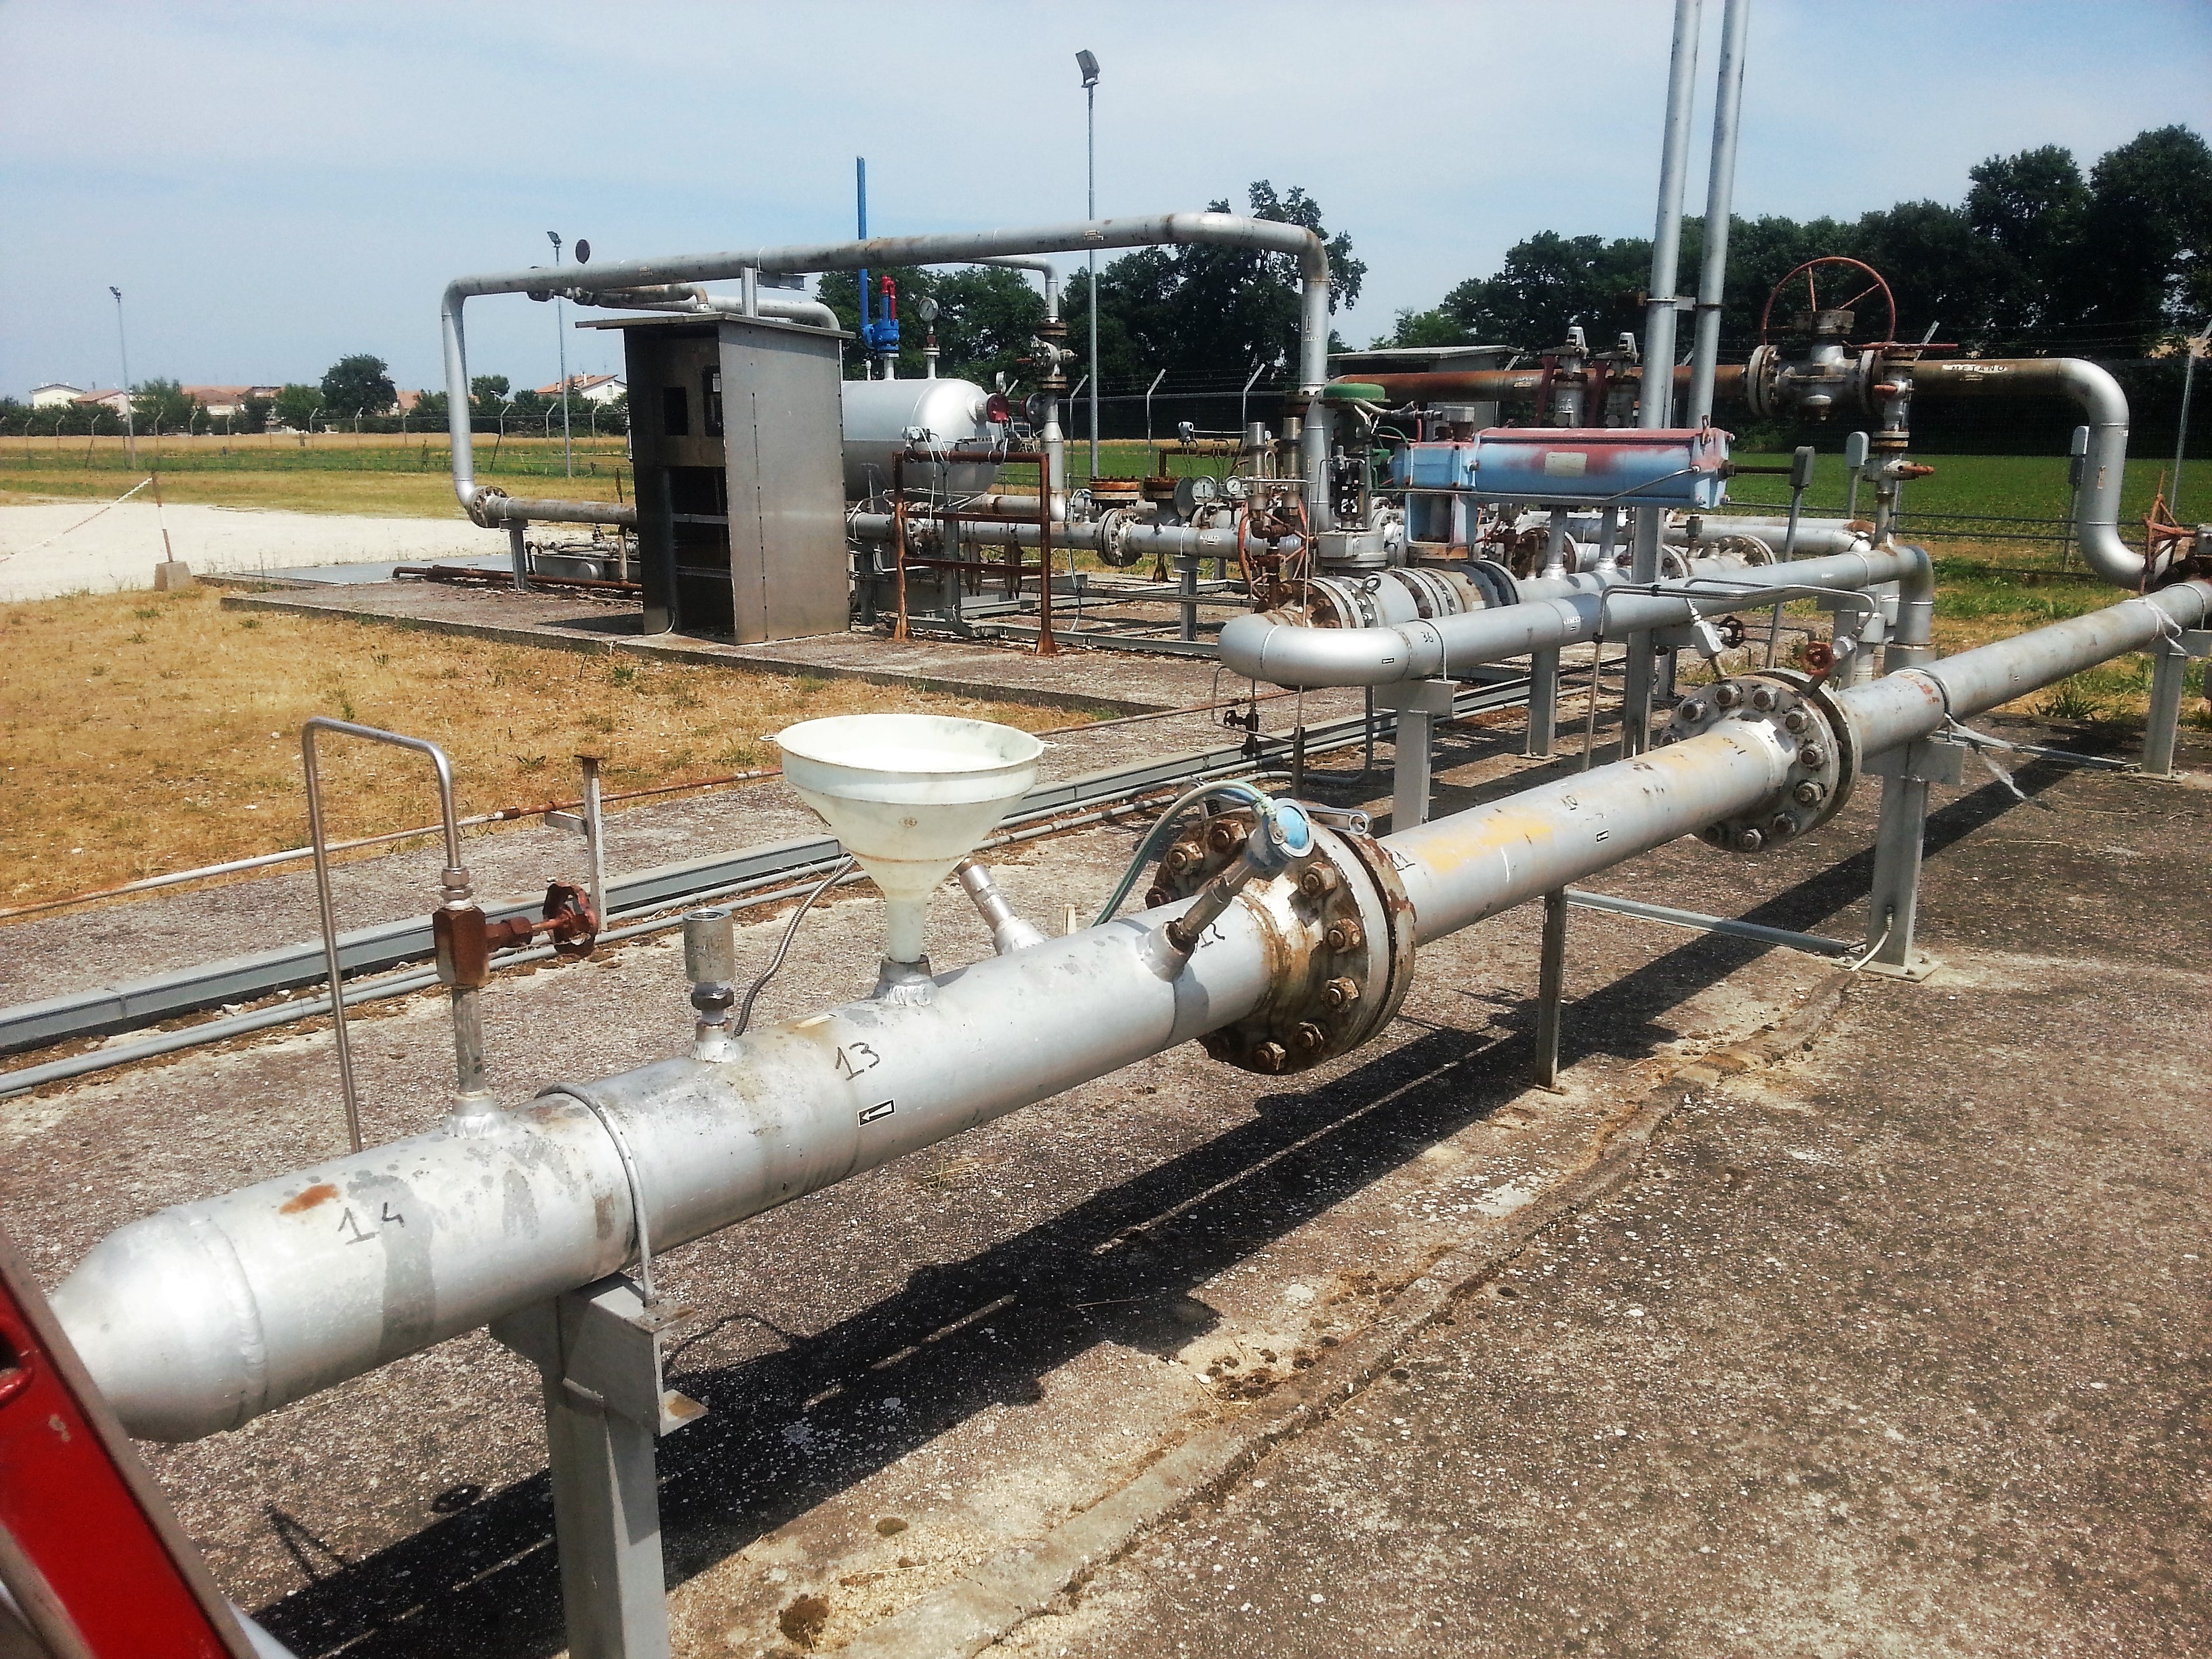
\includegraphics[height=.27\textheight]{fig/test/batch-1} \label{fig:test-batch-immissione}} \qquad   
    \subfloat[][Valvola Fisher, valvola regolatrice associata a un restringimento della condotta.]
    {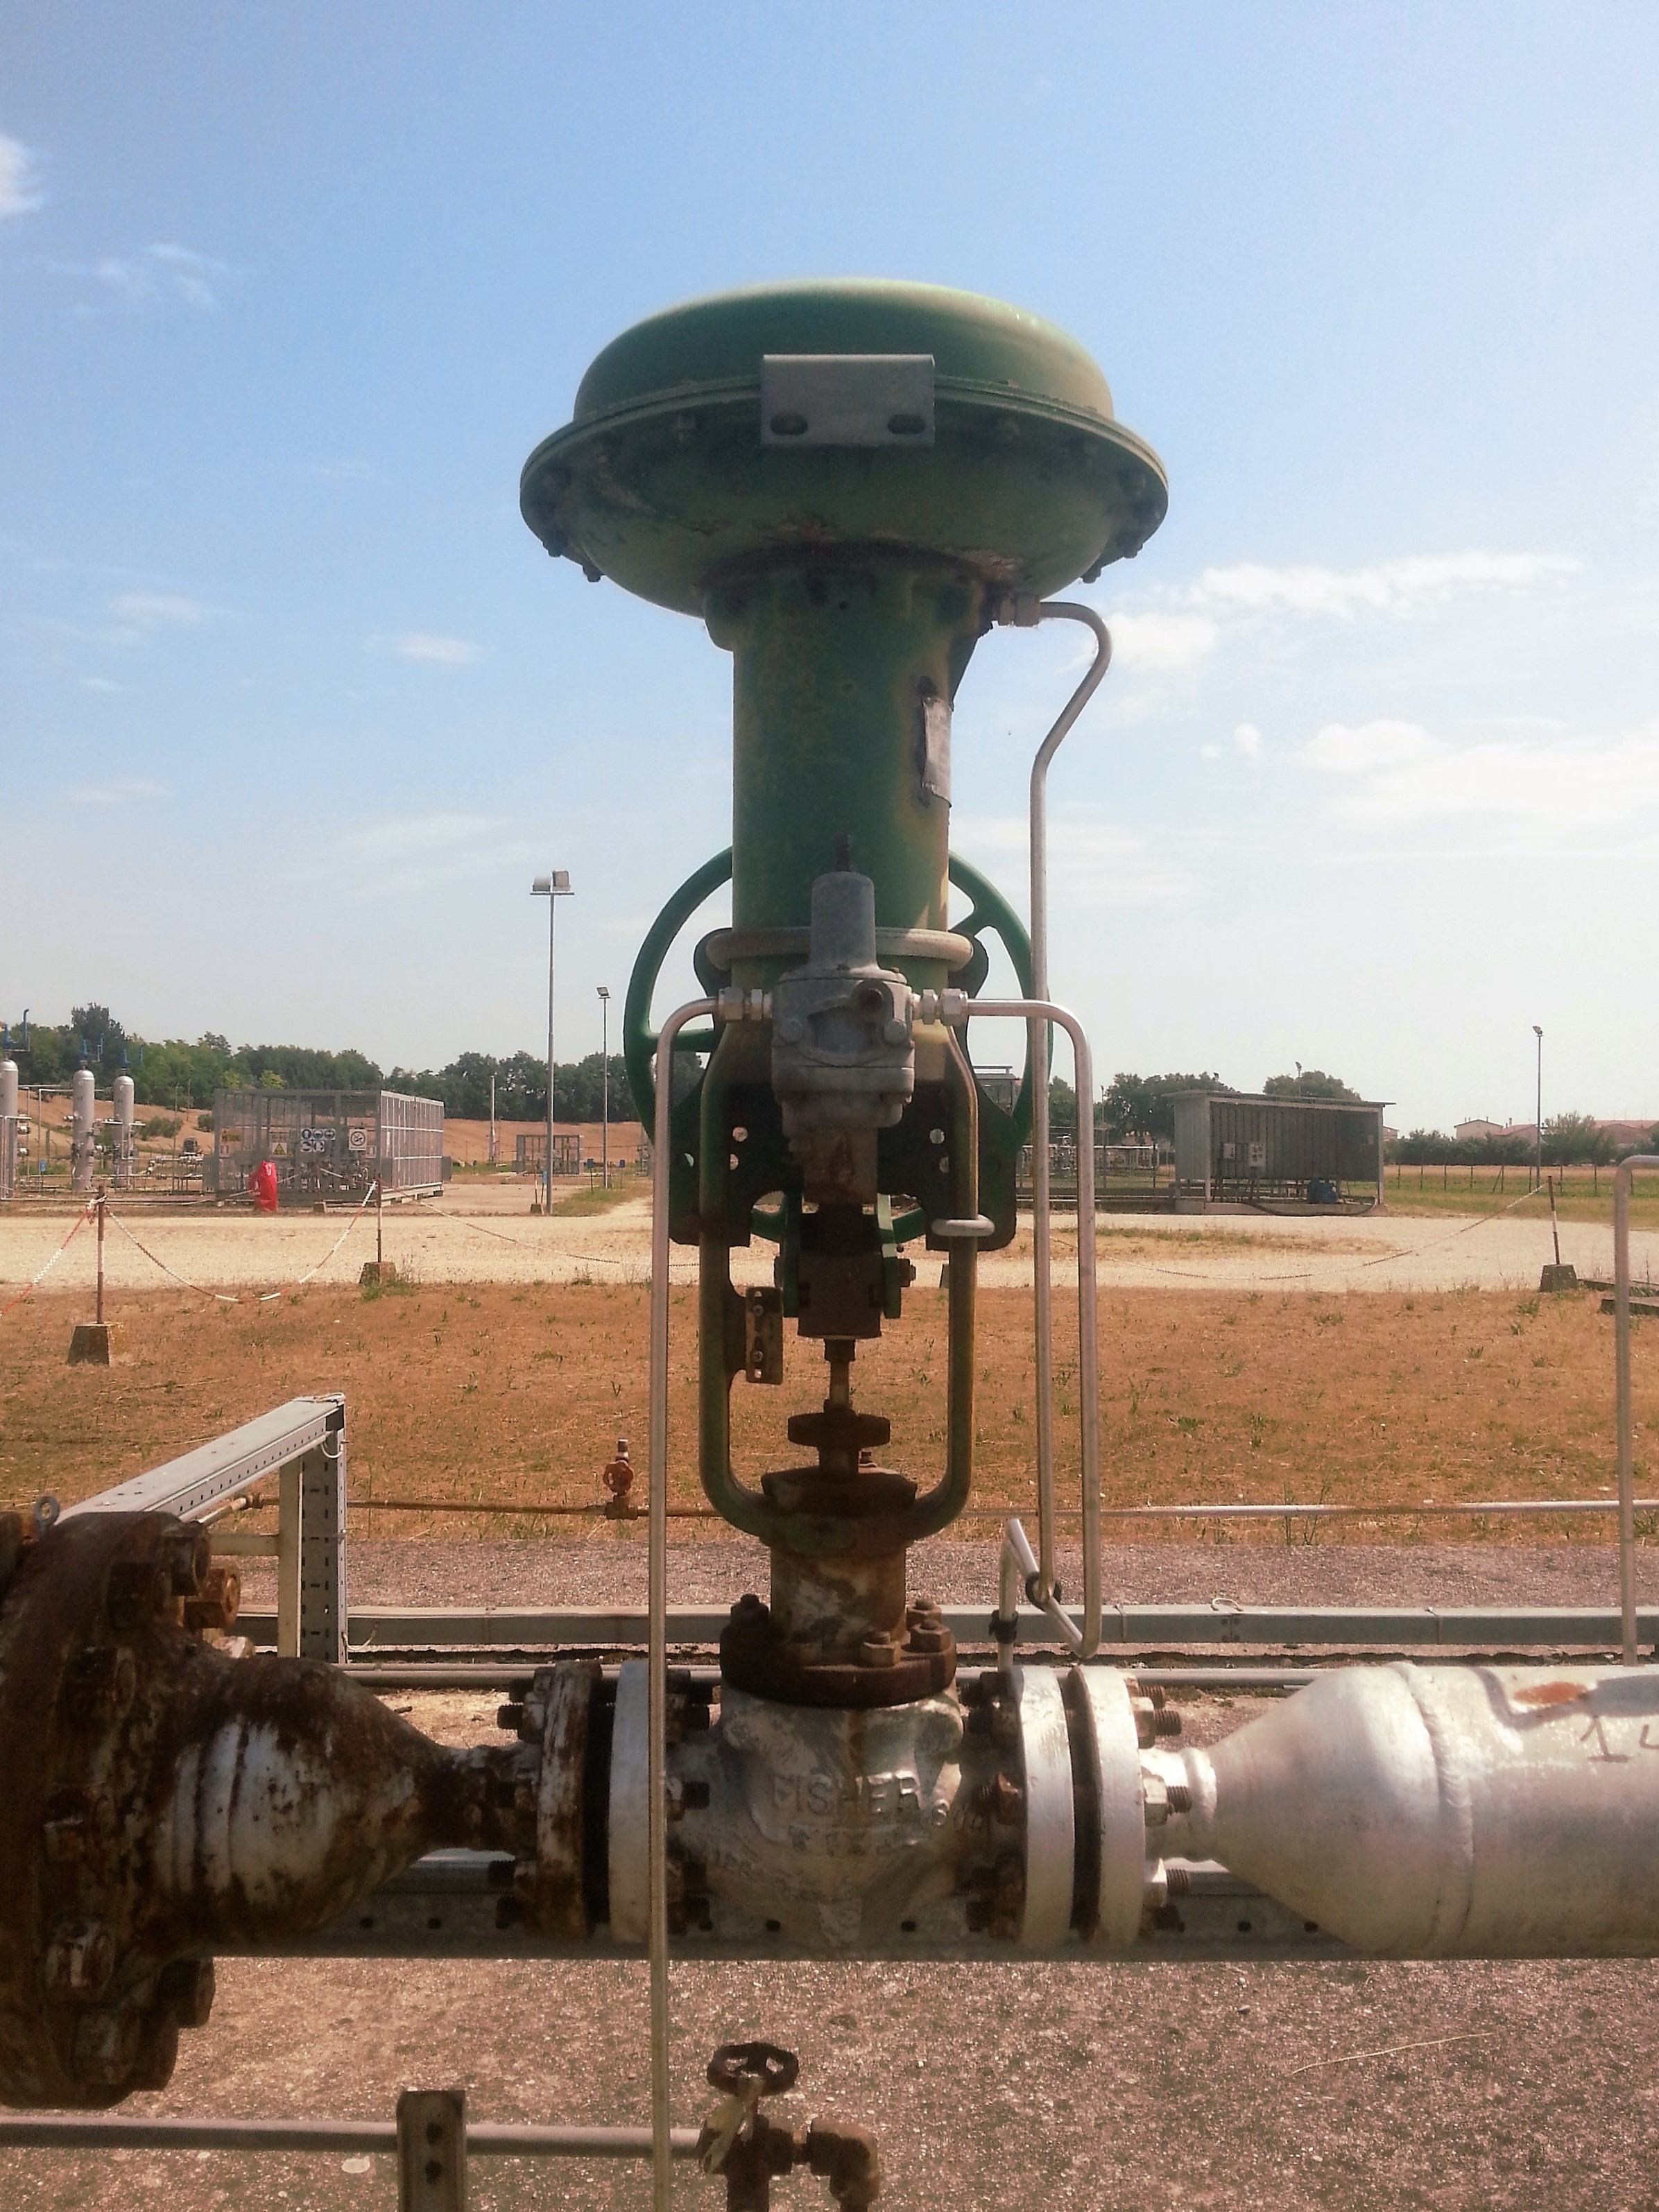
\includegraphics[height=.27\textheight]{fig/test/fisher} \label{fig:test-batch-fisher}}
\caption{Applicazione di schiumogeno in-batch: immissione e dettaglio della PCV.}
\label{fig:test-batch}
\end{figure}

%-----------------------------------------------------

\subsection{Iniezione in continuo}
Lo schiumogeno è stato iniettato in continuo tramite una pompa volumetrica(\figref{fig:test-continuo-pompa}). La macchina è collocata aLa potenza massima della pompa è di 8 litri orari; la portata è stata impostata a 4 litri orari, sfruttando così il 50\% della potenza massima della macchina.

\begin{figure}[htbp]
    \centering
\subfloat[][Pompa volumetrica installata nei pressi della cisterna IBC.]
    {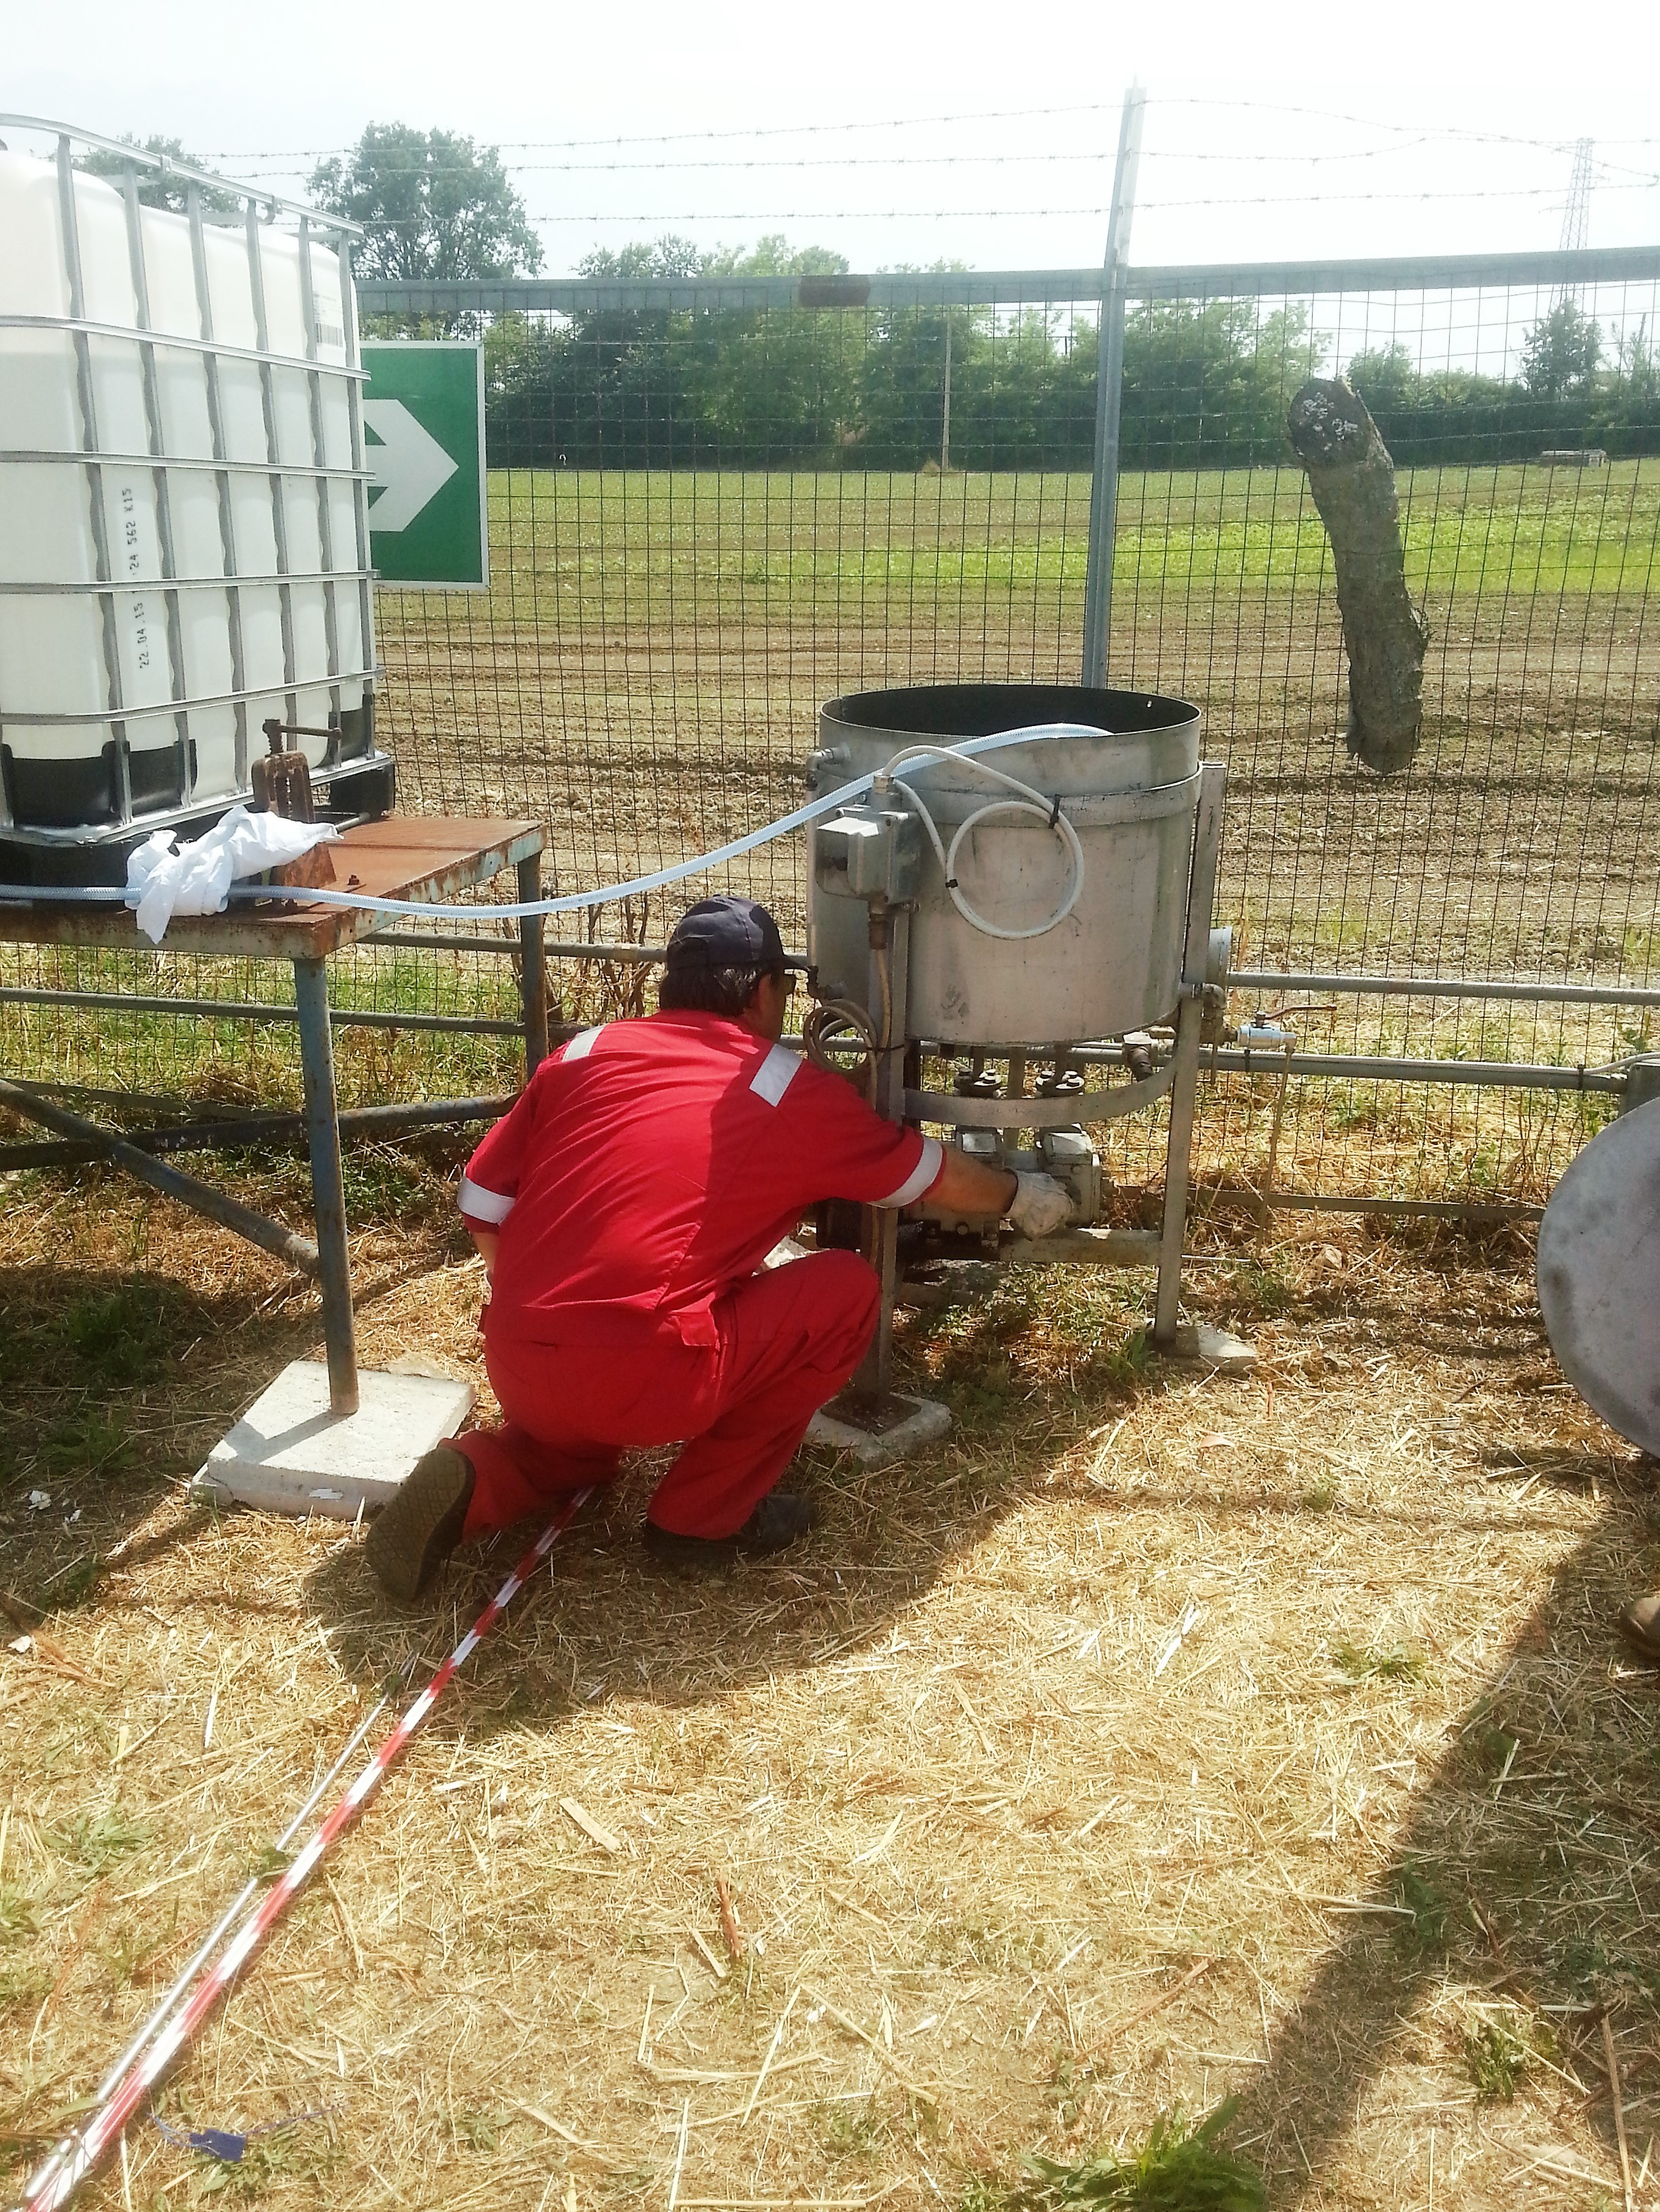
\includegraphics[height=.27\textheight]{fig/test/continuo-1} \label{fig:test-continuo-pompa}} \qquad   
    \subfloat[][Linea di collegamento tra la pompa e la mandata.]
    {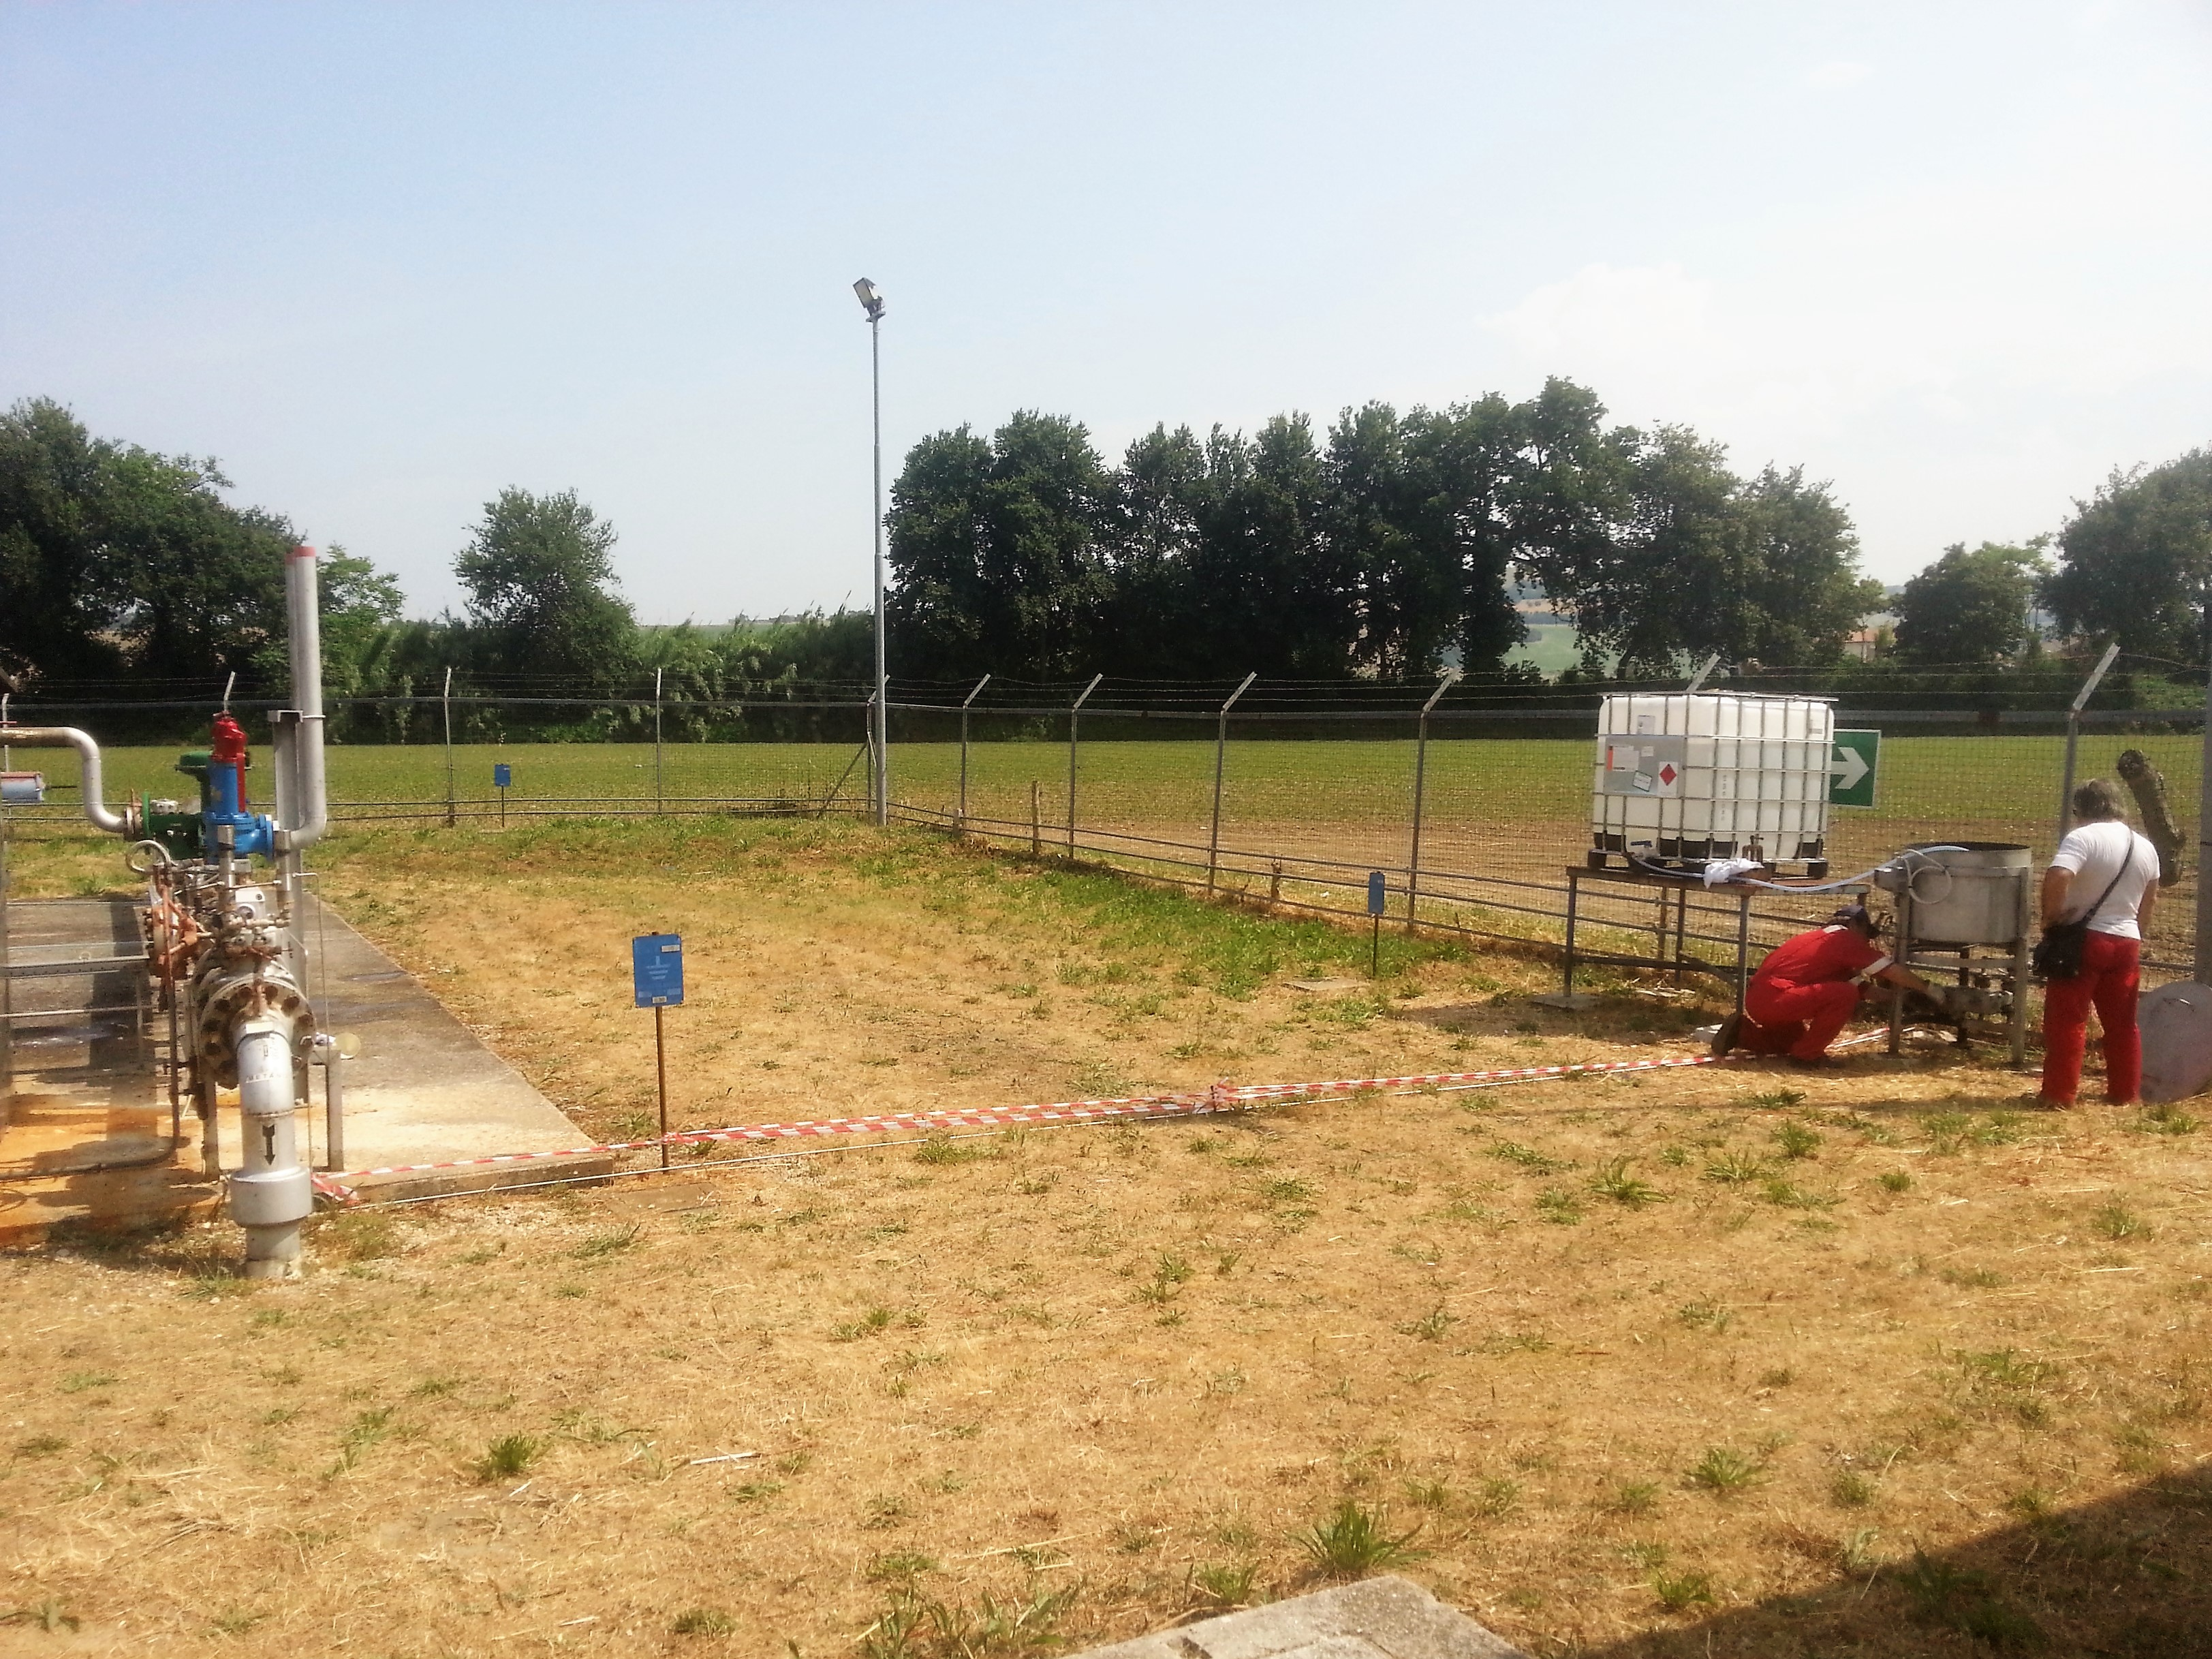
\includegraphics[height=.27\textheight]{fig/test/continuo-2} \label{fig:test-continuo-linea}}
\caption{Immissione dello schiumogeno in continuo.}
\label{fig:test-continuo}
\end{figure}

L'immissione del batch di schiuma sarebbe potuta essere non necessaria in presenza di una pompa a maggiore potenza. Maggiori dosaggi nell'intervallo di tempo avrebbe potuto garantire lo shock iniziale del sistema, quindi l'attivazione della soluzione acqua-schiumogeno nel primo avvallamento. (\figref{fig:continuo-model}). Una volta attivato il \textit{foamer} nel primo avvallamento, una maggiore potenza della pompa avrebbe garantito concentrazioni sufficienti anche per l'acqua nel secondo avvallamento, che nel frattempo sarebbe entrata in soluzione con il primo cuscino d'acqua.\\
La pompa è stata avviata al termine delle operazioni di batch dello schiumogeno.

\begin{figure}[htbp]
    \centering
    \subfloat[][Arrivo dello schiumogeno sulla prima condotta.]
    {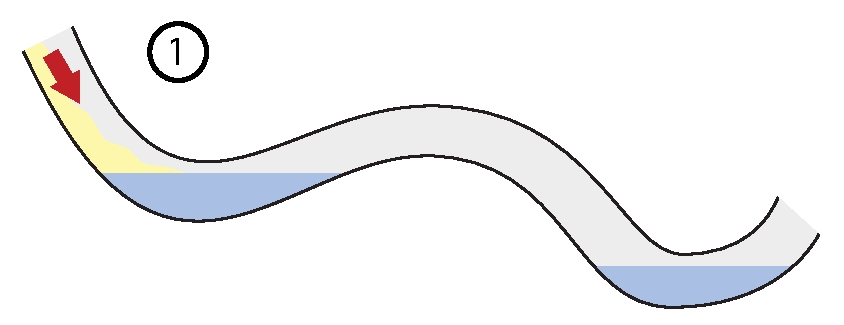
\includegraphics[width=.45\textwidth]{fig/test/continuo-model-1.eps}  \label{fig:batch-1}} \qquad
    \subfloat[][Attivazione dello schiumogeno e trasporto della schiuma nel secondo avvallamento.]
    {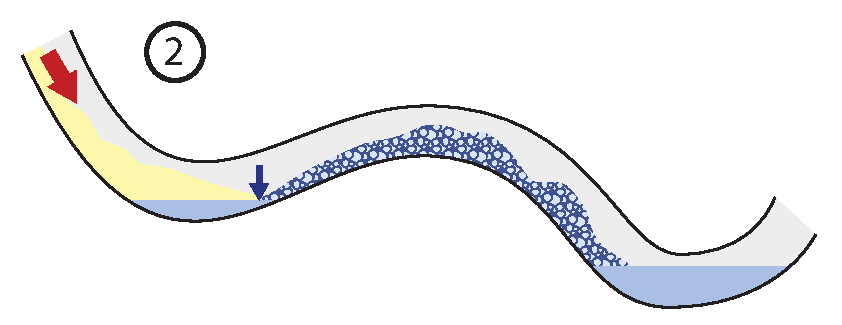
\includegraphics[width=.45\textwidth]{fig/test/continuo-model-2.eps} \label{fig:batch-2}} 
\caption{Principio di funzionamento dello schiumogeno in continuo. Al fine di mantenere una concentrazione minima di attivazione si applica un batch di \textit{foamer} iniziale.}
\label{fig:continuo-model}
\end{figure}

\subsection{Controllo della schiuma in centrale}
Per l'iniezione di \textit{defoamer} è stata impiegata una pompa esterna appositamente allestita per l'esecuzione del test. L'iniezione è avvenuta a sul separatore S-111 tramite una valvola a monte della relativa PCV utilizzata in passato per l'immissione di prodotti chimici come anticorrosivi o biocidi.\\
La schiuma all'interno del separatore non può essere rilevata dalle valvole di alto livello. In caso di aumento incontrollato del livello, la schiuma può oltrepassare il separatore e creare problemi di varia natura a tutto l'impianto, a cominciare dai compressori subito a valle.\\
La pompa dosatrice è stata attivata 30 minuti dopo l'inizio delle operazione legate al batch di schiumogeno. La portata di immissione era di 30 litri orari.

%\begin{figure}[htbp]
%    \centering
%    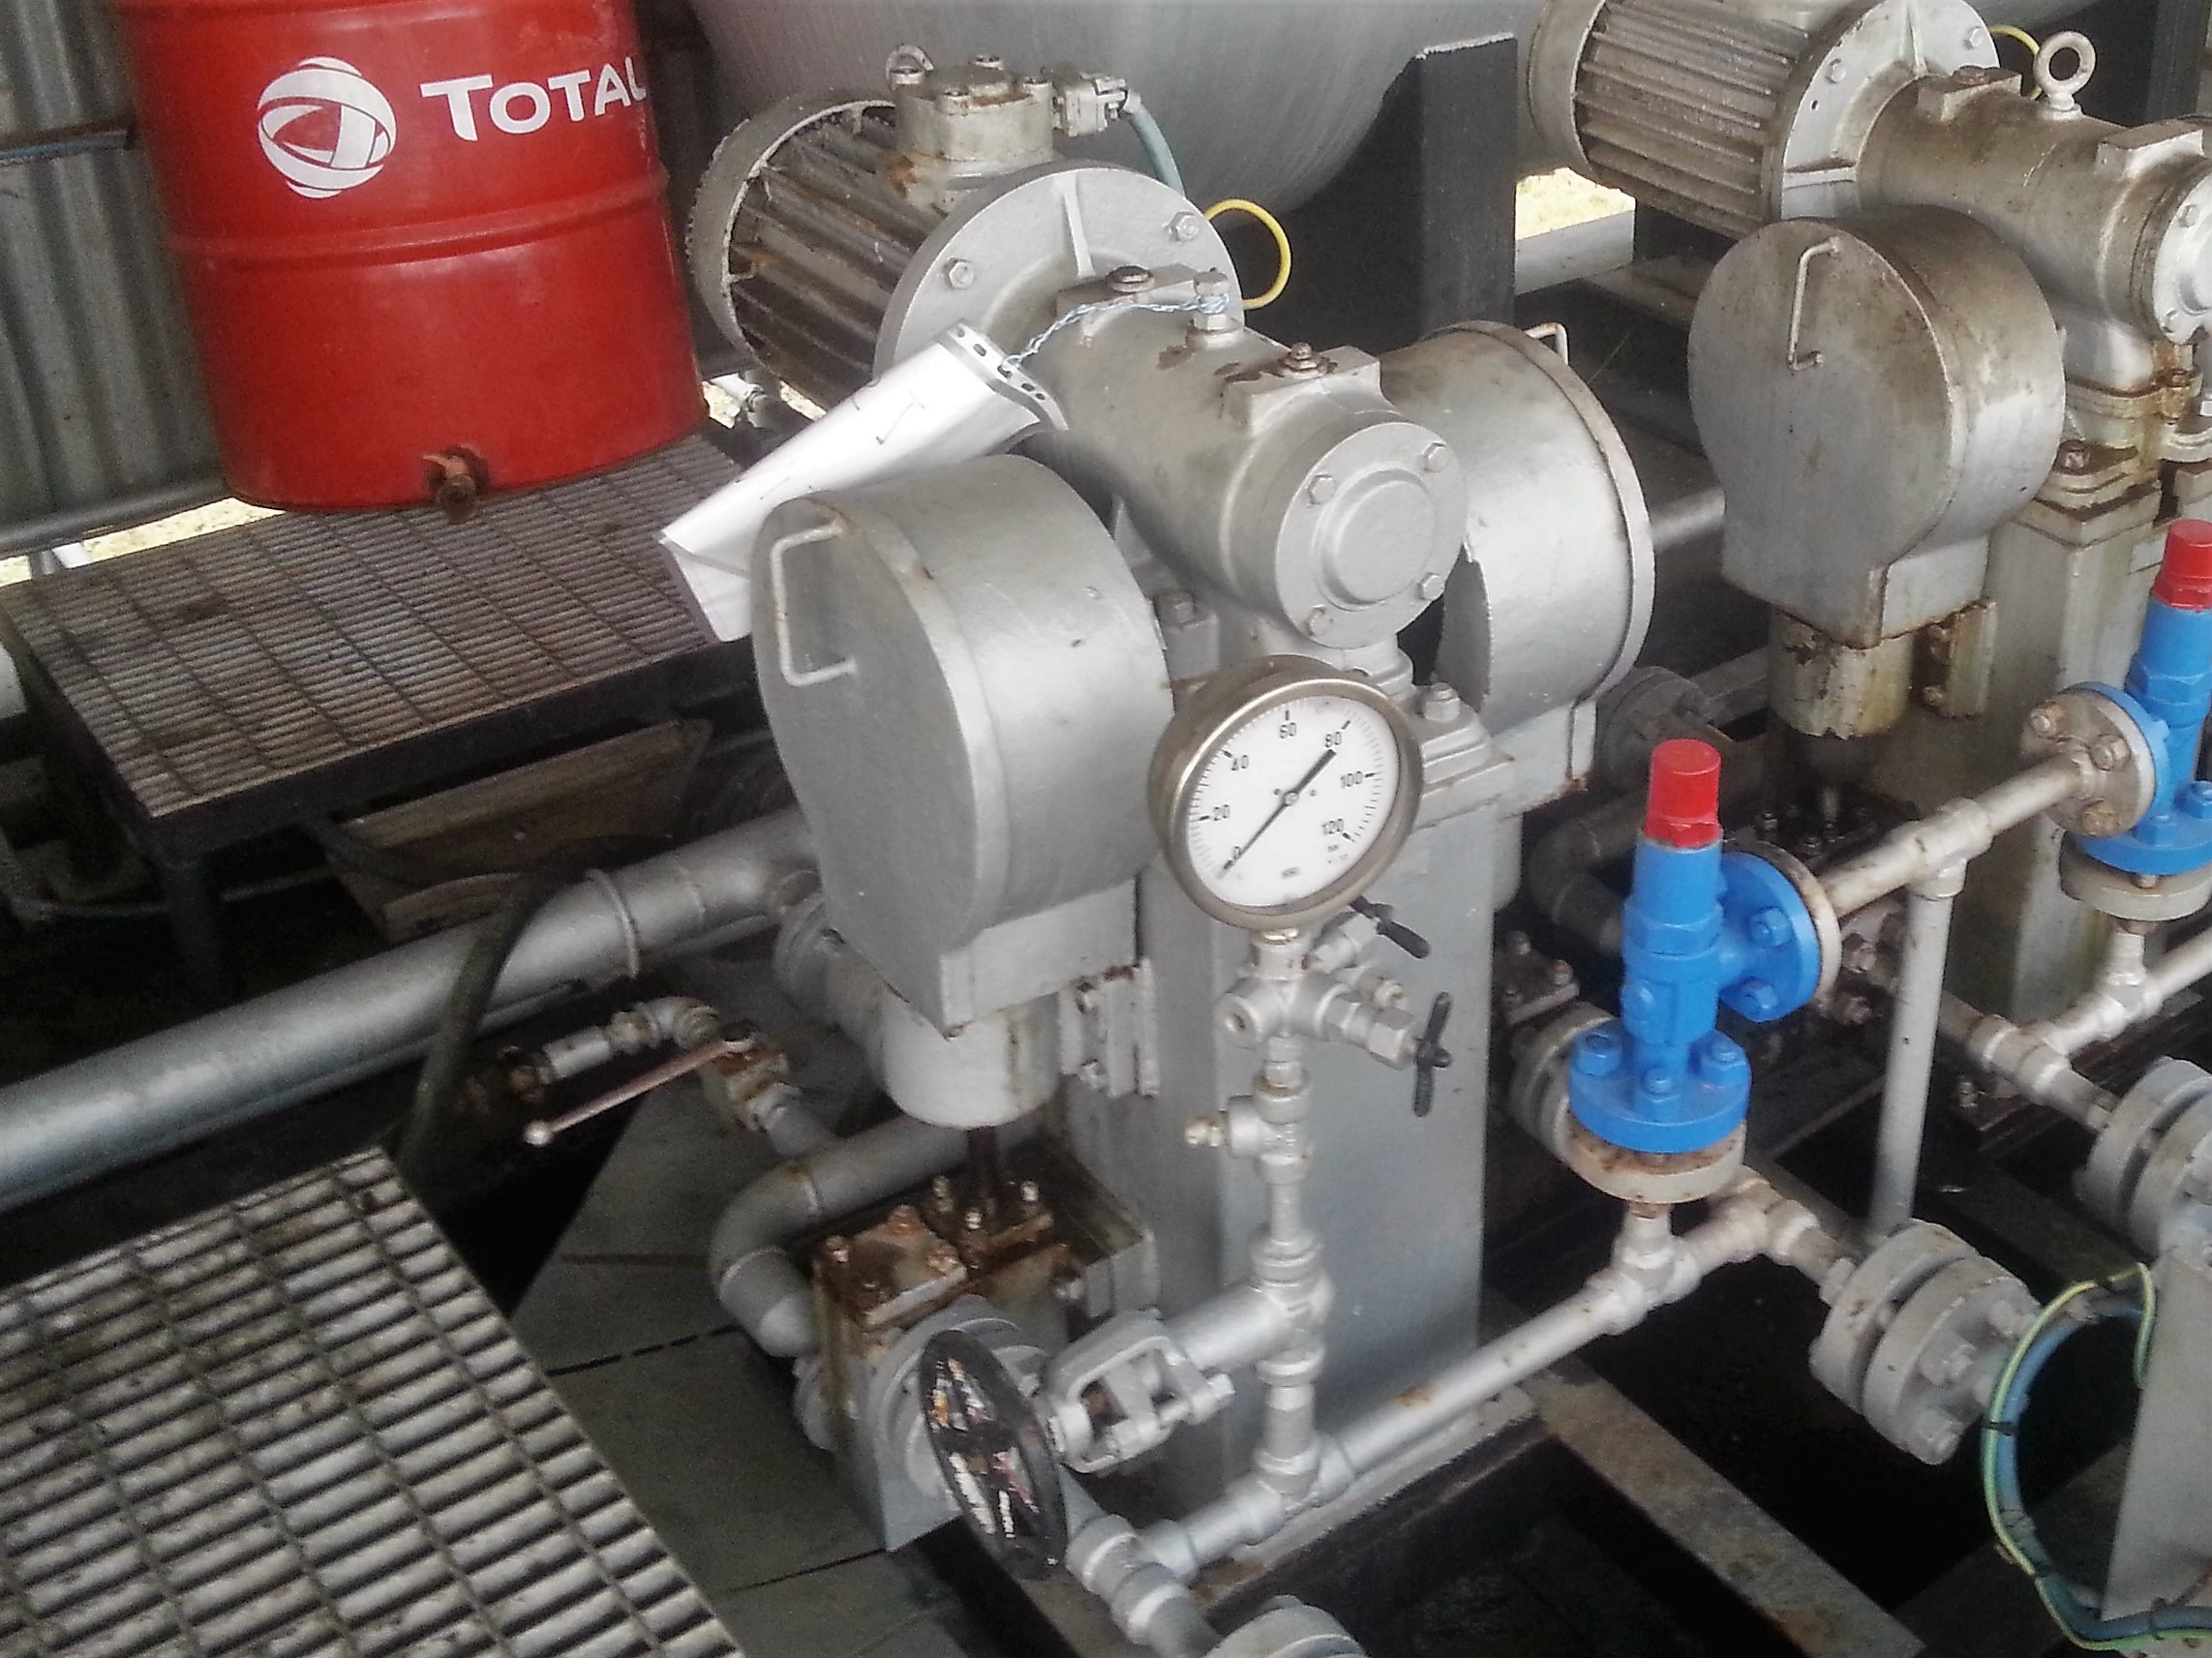
\includegraphics[width=.5\textwidth]{fig/test/pompa-defoamer}
%    \caption{Pompa dosatrice impiegata per l'iniezione dell'antischiuma nel separatore.} 
%    \label{fig:pompa-antischiuma}
%\end{figure}

\subsection{Apparati di misura}
I parametri di pressione e temperatura sono stati monitorati tramite un termomanometro digitale installato sulla linea di mandata, tra la PCV e le valvole di \textit{blow-down}, in corrispondenza dei due \textit{spool} flangiati. Il supporto del termomanometro era inizialmente di 60 minuti. Una volta riscontrata la celerità dell'evento, il supporto è stato portato a un minuto a distanza di 5 ore dall'inizio della misurazione. La pressione assoluta, temperatura e portata sono state inoltre monitorate tramite la strumentazione di impianto (VESCOM 3V), fornendo misure istantanee, e compilando rapporti orari e giornalieri.

\section{Risultati e discussione}
Dalle conoscenze tecniche del prodotto e dall'esperienza acquisita nel precedente pozzo Cozza, lo spiazzamento dell'acqua e i suoi relativi volumi sarebbero stati apprezzabili nell'ordine di decine di ore. Lo schiumogeno reagisce con l'acqua solo al raggiungimento della concentrazione di attivazione \(c_{f}\) di 5000 ppm, valore che l'acqua accumulata avrebbe dovuto raggiungere in tutti gli avvallamenti della condotta (4 totali) prima di defluire alla centrale SGM. In questo caso l'acqua non è confluita con portata costante, bensì lo spiazzamento si è realizzato in un cuscino unico fluido, seguito da una modesta portata nelle ore successive.
\subsection{Studio degli effetti a breve termine}
Dopo un'attesa di 2 ore e 10 minuti dall'applicazione del batch, sono confluiti circa 7 m\ap{3} (con una portata stimata di circa 80 m\ap{3}/h) di acqua mista a schiuma (\figref{fig:test-arrivocentrale})e residui solidi di colore scuro, associati all'attività di corrosione interna della condotta.

\begin{figure}[htbp]
    \centering
    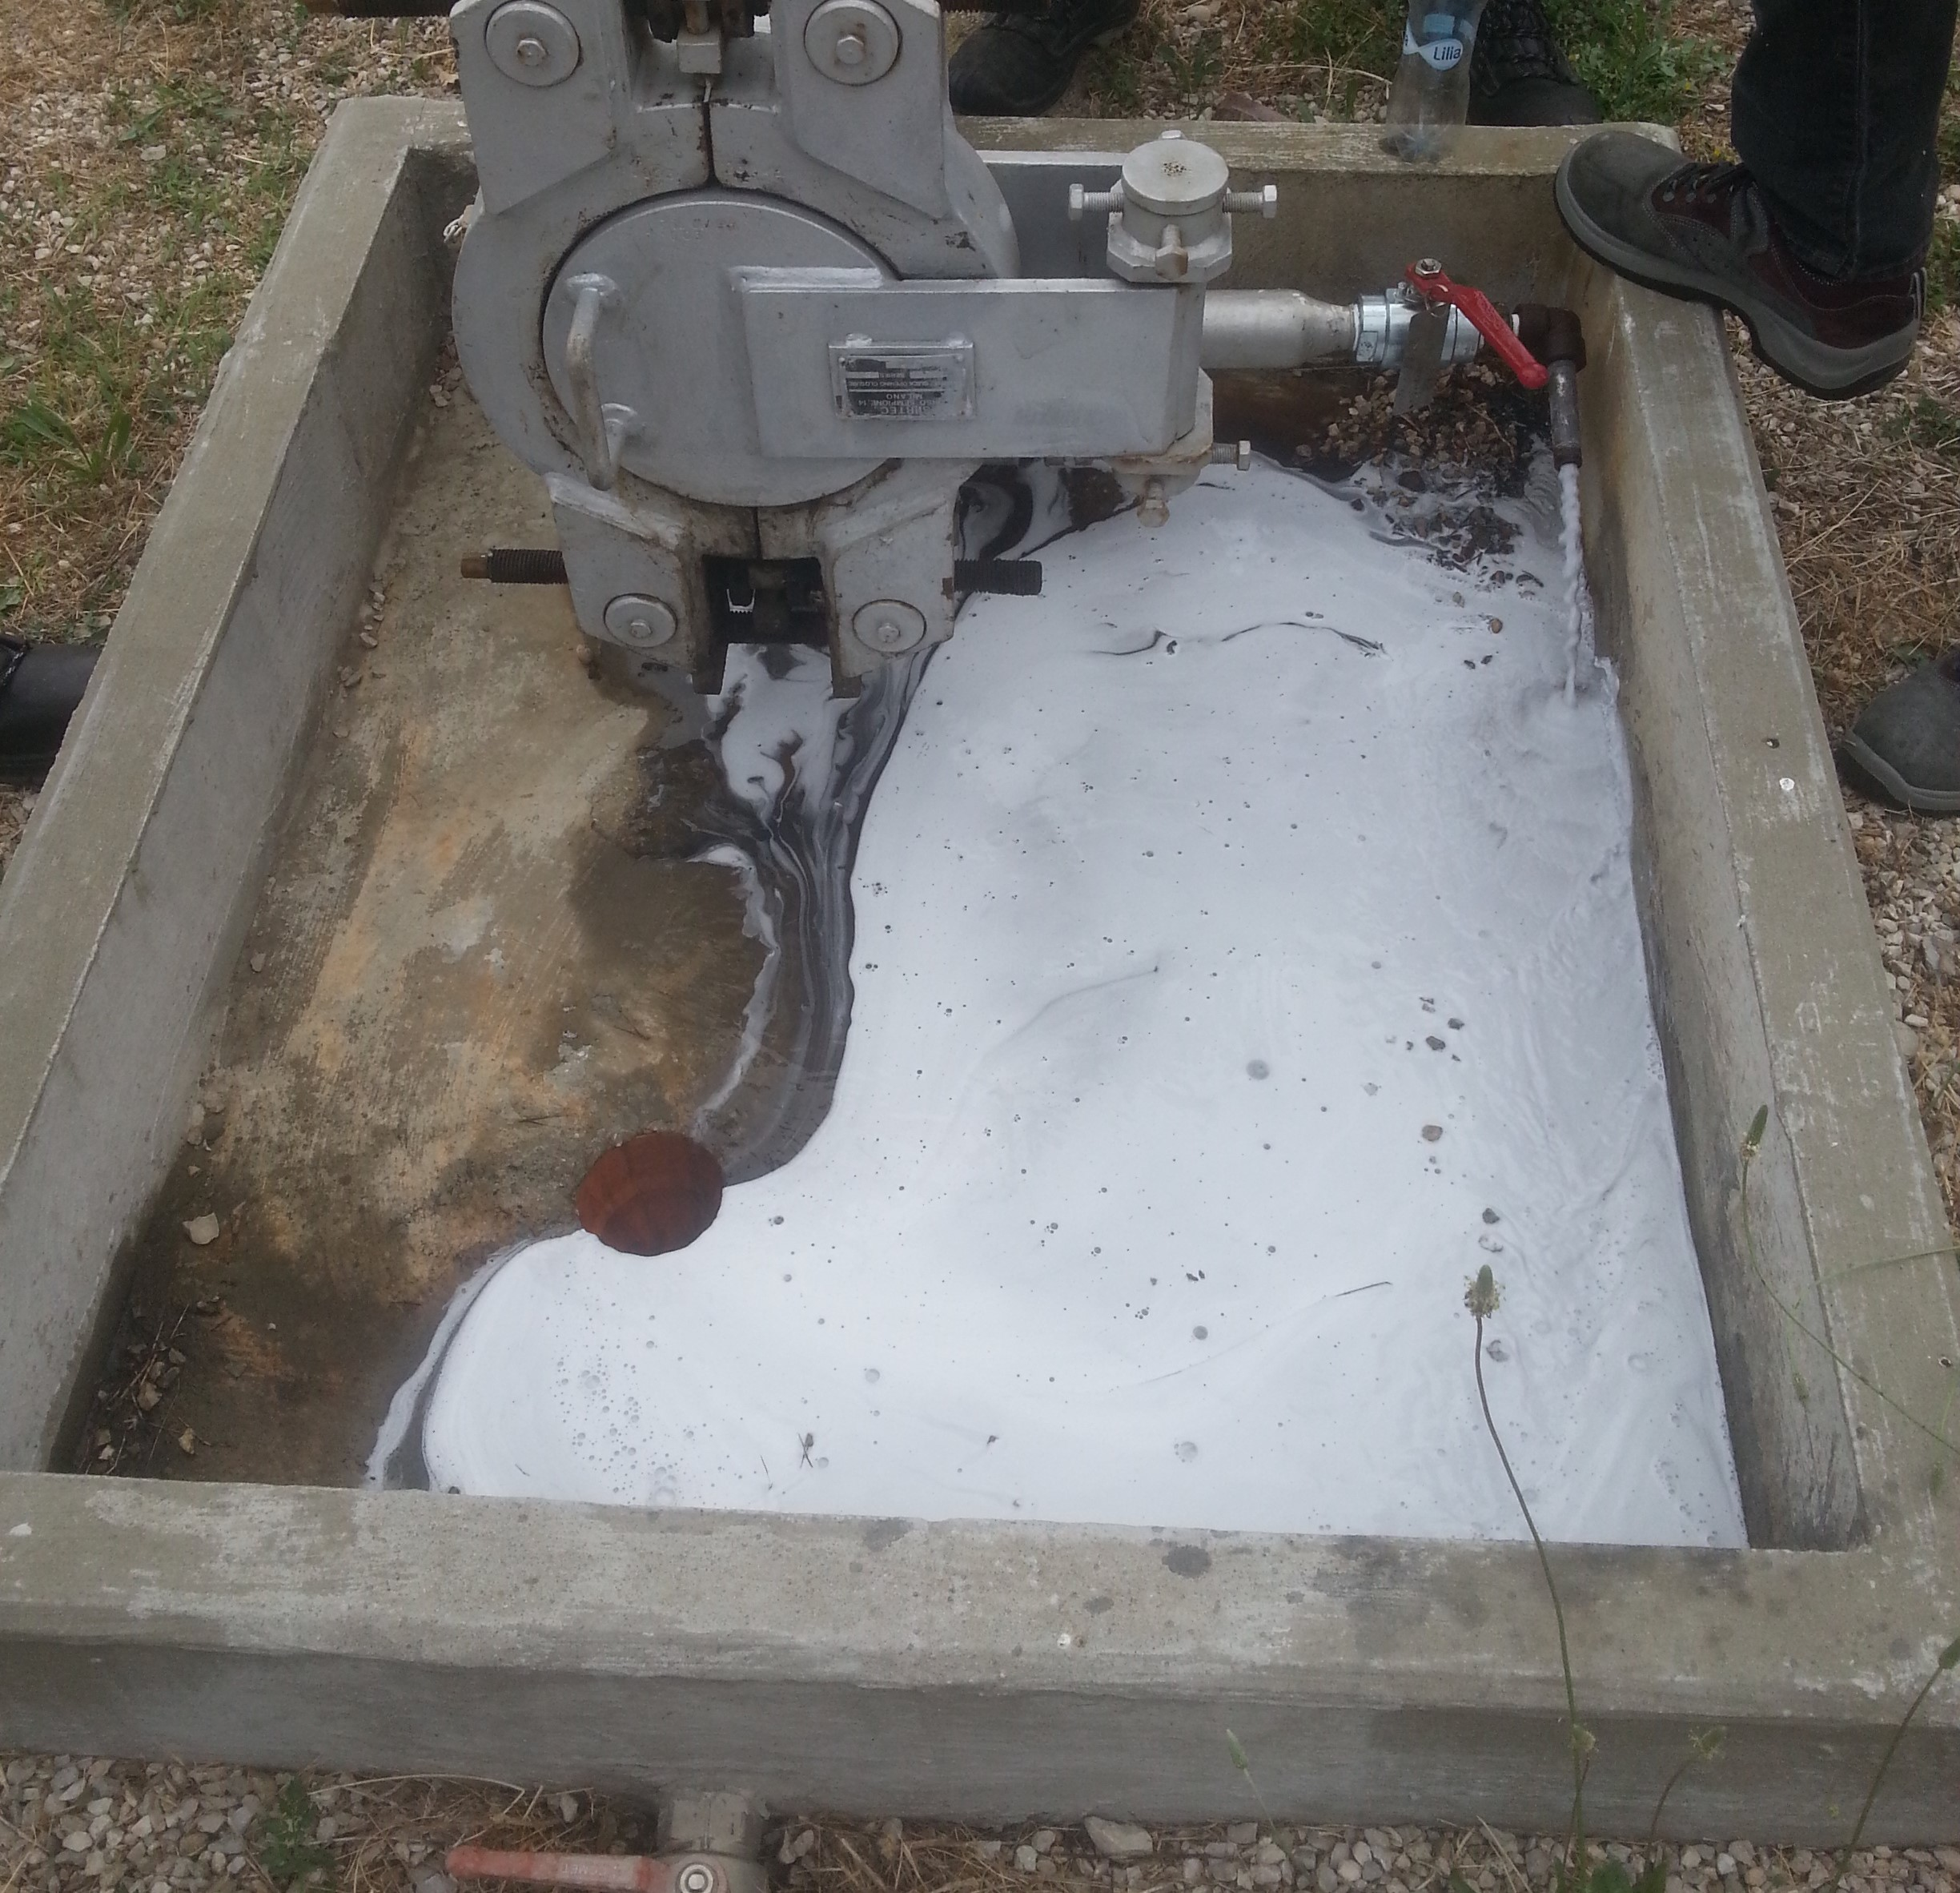
\includegraphics[width=.5\textwidth]{fig/test/arrivo-centrale}
    \caption{Arrivo di acqua in centrale mista a schiuma e polvere nera in soluzione.} 
    \label{fig:test-arrivocentrale}
\end{figure}


L'arrivo improvviso dell'acqua ha portato al blocco centrale a causa della chiusura della valvola di alto livello del separatore S101. Il volume di 7 m\ap{3} deriva dall'acqua accumulata lungo la condotta. Una volta riattivata la produzione a pieno regime, l'afflusso d'acqua è continuato con quantitativi importanti per le successive 2 ore (circa 3 m\ap{3}/h), per poi affievolirsi nell'ordine di decine di litri ora. Il livello della vasca di raccolta acque S117 si è innalzato durante il test di 65 cm, valore legato al volume di acqua confluita in centrale, pari a 12,74 m\ap{3}. Il volume di acqua arrivato in centrale è più che allineato alla quantità di acqua spiazzata con il piggaggio della linea il 30 luglio 2013 (14,5 m\ap{3}).\\
In realtà l'innalzamento della vasca è continuato anche durante la notte. Tuttavia al S117 confluisce anche l'acqua di produzione proveniente dal pozzo Vongola. Si è quindi scelto di applicare un \textit{cut-off} nel momento in cui i trend di produzione dell'acqua sono tornati a valori consueti. Si considera quindi l'innalzamento del battente idrostatico a circa tre ore dall'arrivo in centrale.\\
Nell'arco di tempo tra l'avvio della produzione \textit{post-batch} e l'arrivo dell'acqua in centrale, la pressione in linea ha oscillato attorno a 14 bar. L'oscillazione è riconducibile alla presenza degli avvallamenti, i quali creano queste pulsazioni di pressione. Una volta confluito l'ingente volume d'acqua, dopo 9 ore dall'applicazione la pressione in linea è fortemente decresciuta e si è attestata a circa 6 bar. \\
La temperatura della linea misurata dal manometro digitale, una volta eseguito il batch in condotta e aperti nuovamente i pozzi, è scesa bruscamente dai 32°C ai 21°C circa, testimoniando così l'espansione del gas una volta riaperte le valvole. Durante il test non si riscontrano particolari episodi: la temperatura del termomanometro digitale ha successivamente seguito i trend di quella esterna, rimanendo più o meno costante durante le ore notturne e aumentando durante le ore diurne.\\

\begin{figure}[htbp]
    \centering
    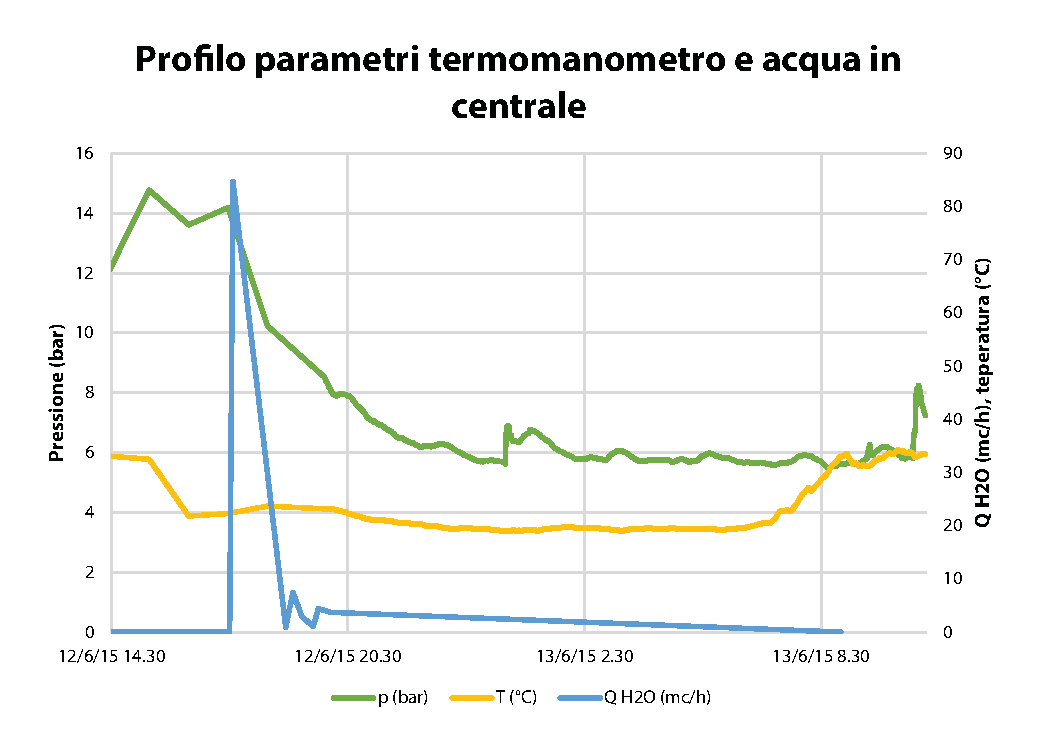
\includegraphics[width=\textwidth]{fig/test/graphs/profili.eps}
    \caption{Variazione della pressione e temperatura misurato sulla mandata di San Marco, in relazione alla portata d'acqua confluita presso la centrale SGM} 
    \label{fig:test-profili}
\end{figure}

L’antischiuma o \textit{defoamer} Phoenix 8161 ha agito correttamente. Al fine di valutare qualitativamente l’azione dell'antischiuma è stata prelevata dell'acqua a monte e a valle del separatore (\figref{fig:defoamer-confronto}). I campioni sono poi stati agitati e lasciati riposare. Sebbene la schiuma si crei in entrambi i contenitori, il fluido a monte del separatore è contraddistinto da una schiuma stabile anche dopo diversi minuti, il fluido a valle invece tende a dissolvere la schiuma presente in superficie nel giro di pochi secondi.

\begin{figure}[htbp]
    \centering
    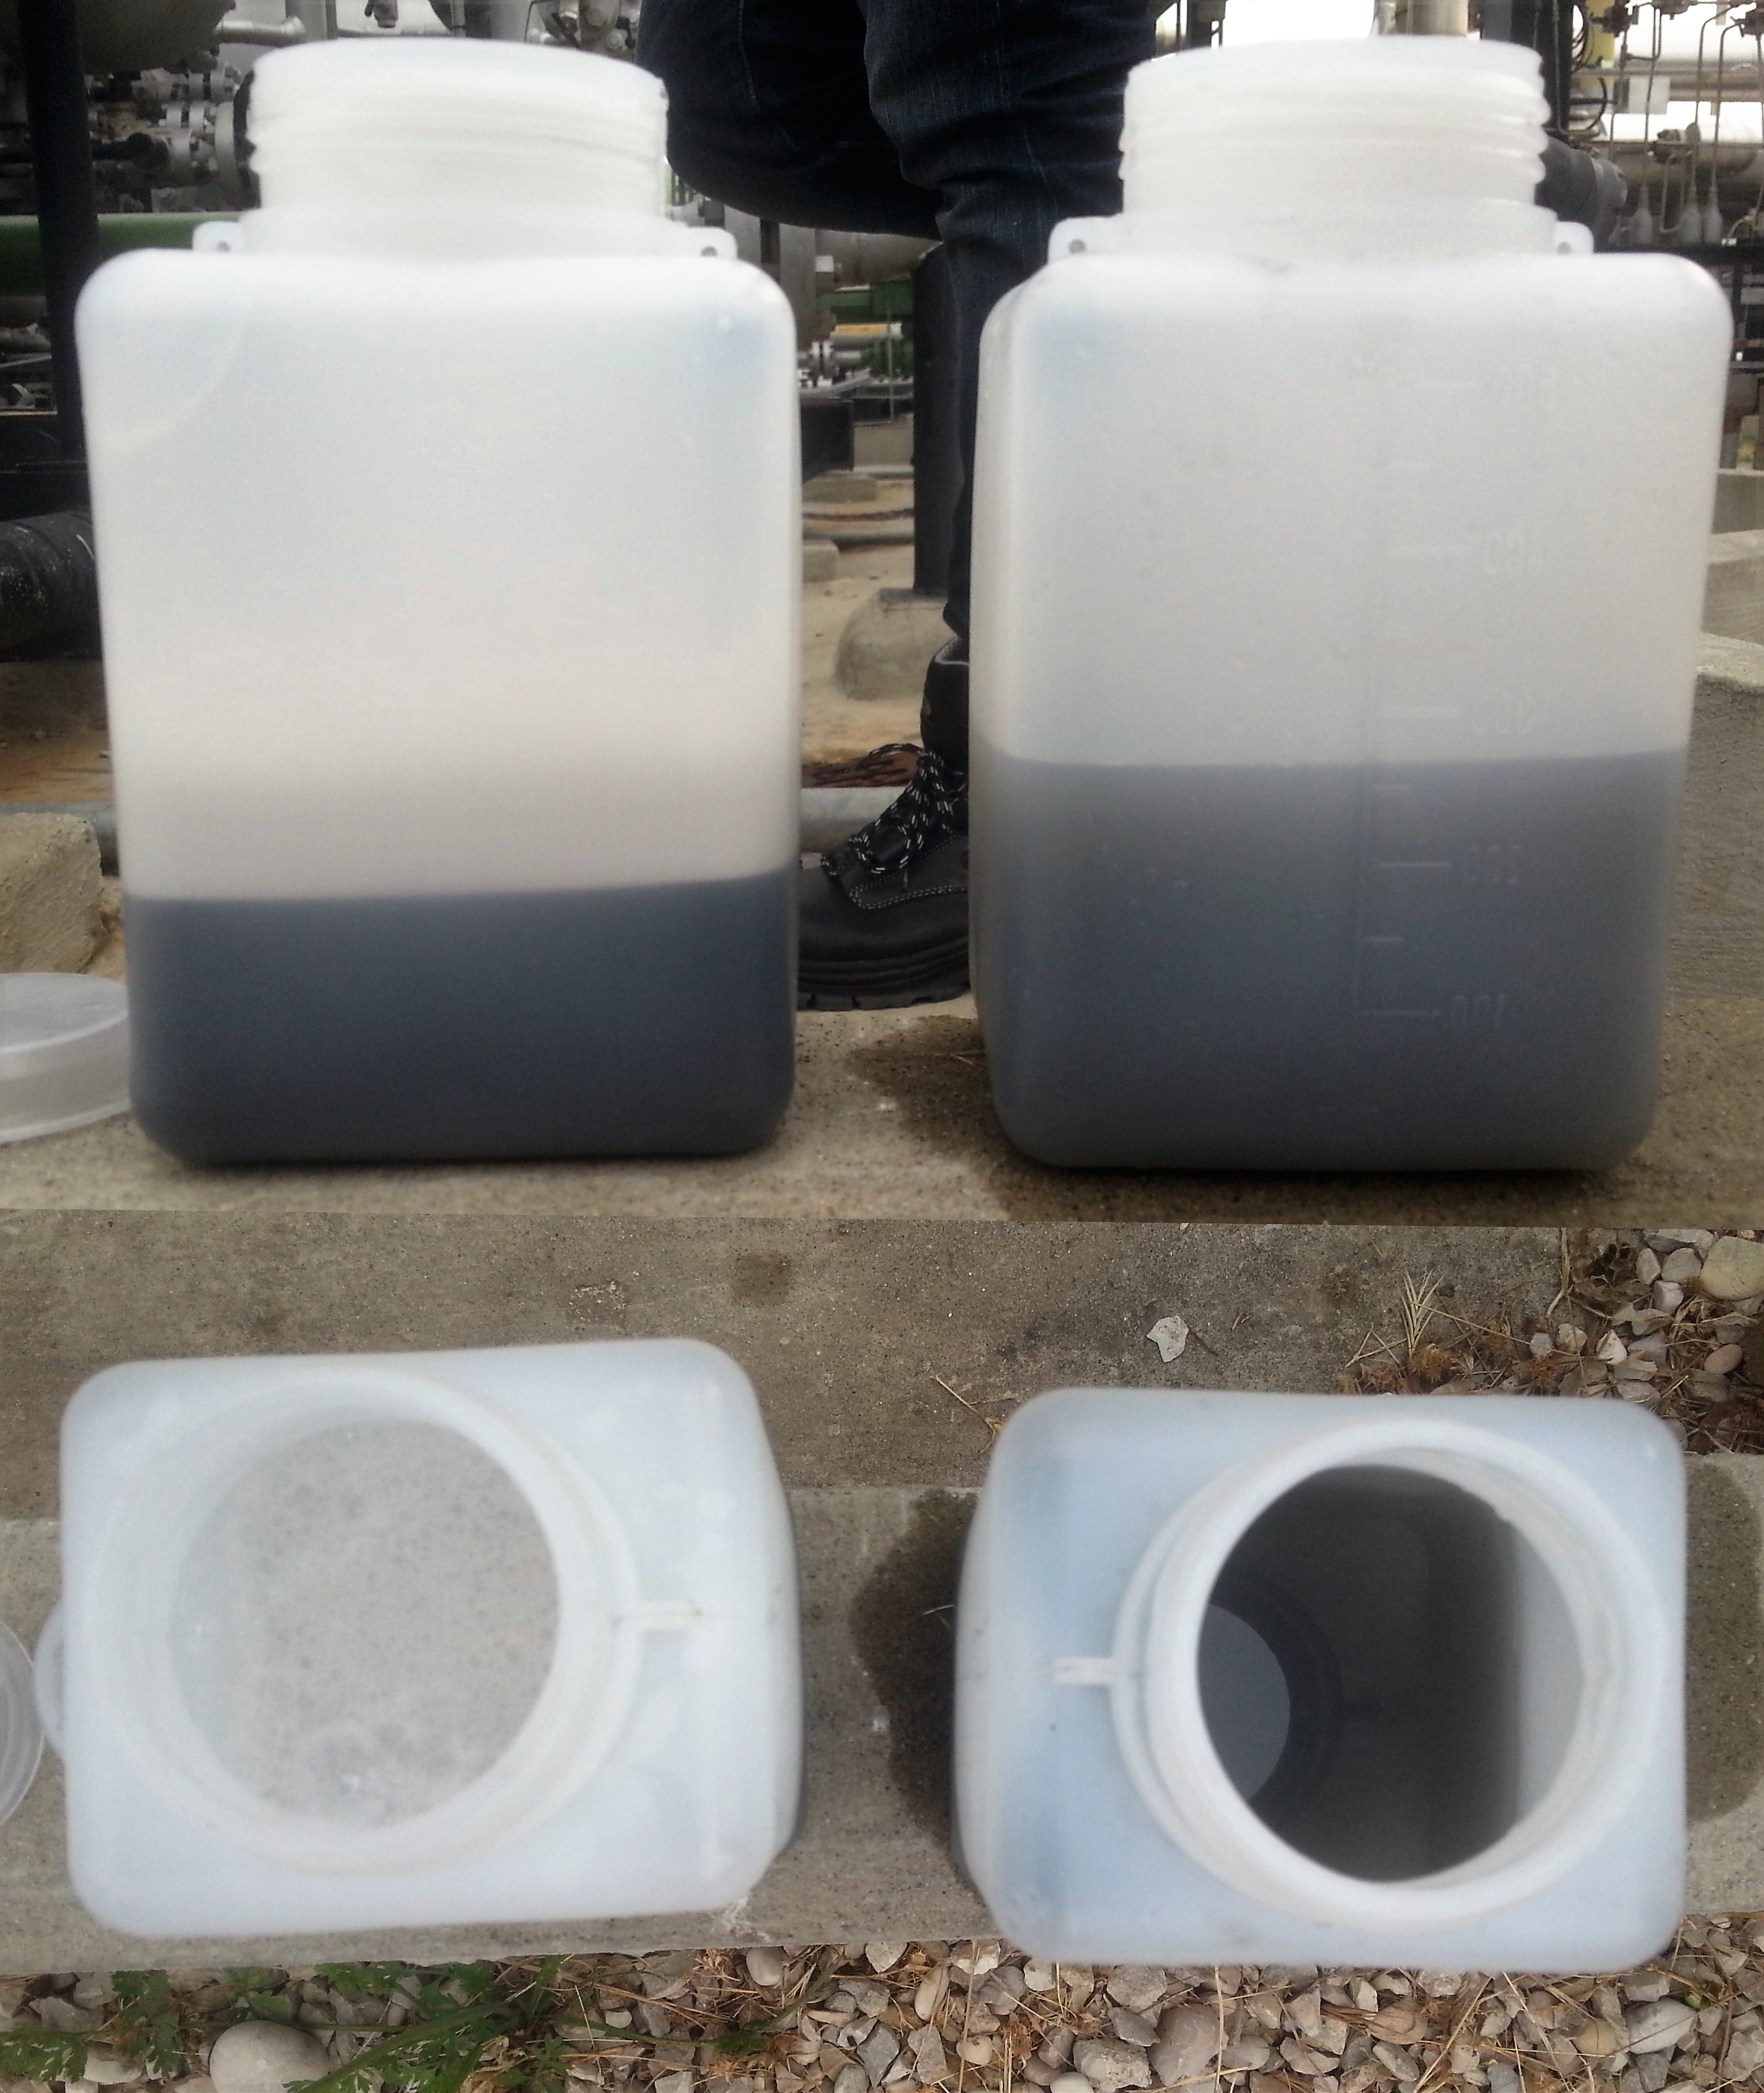
\includegraphics[width=.5\textwidth]{fig/test/defoamer-confronto}
    \caption{Test visivo dell'efficacia dell'antischiuma, da sinistra a destra campioni prelevati rispettivamente a monte e a valle del separatore.} 
    \label{fig:defoamer-confronto}
\end{figure}

\subsection{Andamento produttivo post-test}
Al fine di valutare i vantaggi di tale applicazione, sono stati analizzati nelle settimane successive gli andamenti dei parametri di portata, pressione e acqua prodotta e del pozzo di Verdicchio e dei pozzi e della linea di mandata di San Marco.\\
Preso come riferimento il 12 giugno 2015, giorno in cui è stata effettuata l'operazione di spiazzamento, si considerano due intervalli temporali della durata di 97 giorni, prima e dopo l'applicazione. Gli scenari in questione vanno dal 7 marzo 2015 all'11 giugno 2015 e dal 12 giugno 2015 al 16 settembre 2015.\\
Per quanto riguarda i parametri di pressione, nei pozzi si fa riferimento alla pressione di testa pozzo (PTP o FTHP, \textit{Flowing Tube Head Pressure}), mentre nella mandata il valore esprime la pressione in linea (\textit{Flowing Line Pressure}, FLP).\\
Gli andamenti dei parametri sono valutati tramite grafici, dove è possibile valutare i trend prima e dopo l'applicazione. L'analisi quantitativa dei dati relativi ai due scenari si basa sul calcolo di tre indici statistici: 
\begin{itemize}
\item media aritmetica: \(\mu=\dfrac{1}{n}\sum_{i=1}^n x_i\); 
\item deviazione standard: (della popolazione) \(\sigma= \sqrt{\dfrac{\sum_{i=1}^{n} (x_i-\mu)^2}{n}}\);
\item coefficiente di variazione: \(\sigma\ast= \dfrac{\sigma}{|\mu|}\)
\end{itemize}
dove \(x_i\) sono variabili generiche e \(n\) il numero di variabili della serie generica. Si è scelto di calcolare il coefficiente di variazione, un indice di dispersione che permette di valutare la dispersione dei valori indipendentemente dal valore medio assoluto (è un indice adimensionale)\\
\'E importante sottolineare che dopo l'applicazione, in base ai risultati ottenuti e riportati qui di seguito, è iniziata una fase di ottimizzazione dei pozzi che si innestano a monte della PCV regolando il settaggio della valvola stessa. Immediatamente dopo lo spiazzamento della condotta la pressione della PCV è stata portata da 15 bar a 11 bar. In un secondo, il giorno 7 luglio 2015 la PCV è stata settata da 11 bar a 9 bar.\\
La \figref{fig:prod-totale} mostra che, dopo l'applicazione, la portata di gas naturale della linea Verdicchio (come detto in precedenza, si trascurano i contributi di San Lorenzo e della Centrale MAM) è aumentata del 5,07\%, a testimoniare il fatto che minori contropressioni conseguono migliori condizioni di produzione. L'acqua di produzione non viene mostrata poiché fa riferimento al solo campo di San Marco (Verdicchio è un pozzo anidro).

\begin{figure}[htbp]
    \centering
    \subfloat[][Andamento di portata gas della linea Verdicchio (si omettono San Lorenzo e il gas proveniente dalla centrale MAM) dal 07/03/2015 al 16/09/2015.]
    {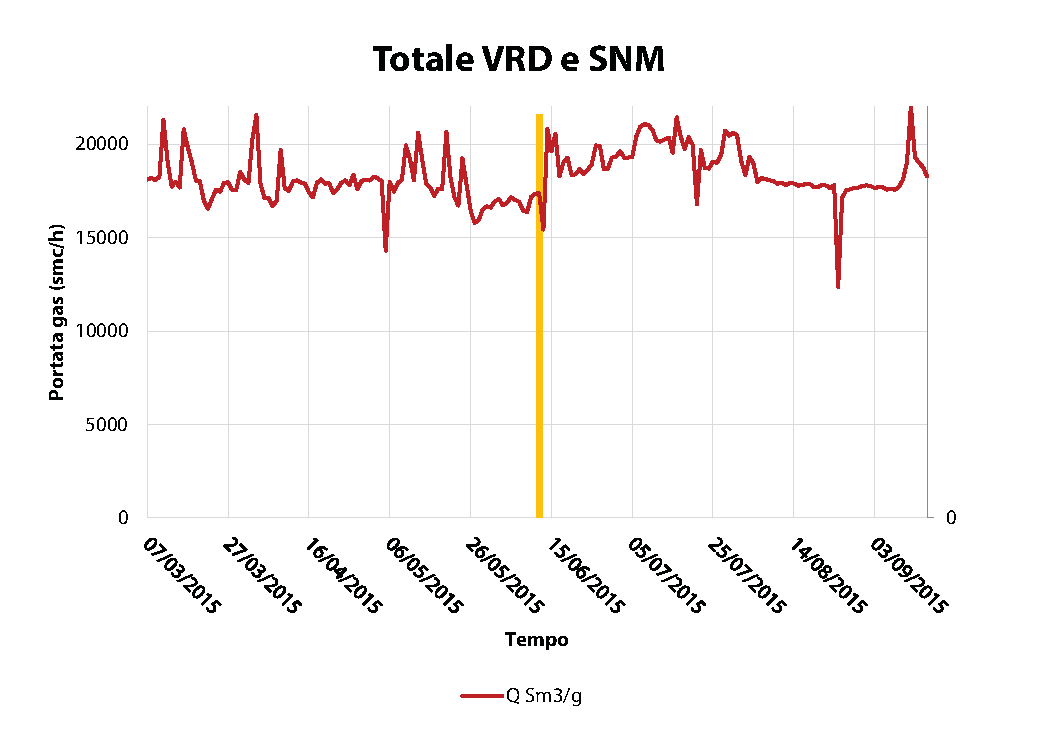
\includegraphics[width=\textwidth]{fig/test/graphs/totale.eps} \label{fig:test-totalegas}}\\
\subfloat[][Indici statistici della portata relativa alla linea Verdicchio (si omettono San Lorenzo e il gas proveniente dalla centrale MAM), periodi 07/03-11/06 e 12/06-16/09.] {
\centering
\footnotesize
\label{tab:totalegas}
\begin{tabular}{l|crrrr|}
\cline{2-6}
                                & Indice stat.         & \multicolumn{1}{c}{\textsc{Pre-test}} & \multicolumn{1}{c}{\textsc{Post-test}} & \multicolumn{1}{c}{\(\mathrm{\Delta}\)} & \multicolumn{1}{c|}{\(\mathrm{\Delta}\)\%} \\ \hline
\multicolumn{1}{|l|}{Gas (Smc)} & \(\mu_{gas}\)        & 17852,34                              & 18758,21                               & 905,866                                 & 5,07\%                                      \\
\multicolumn{1}{|l|}{}          & \(\sigma_{gas}\)     & 1148,53                               & 1370,326                               & 221,7964                                & 19,31\%                                     \\
\multicolumn{1}{|l|}{}          & \(\sigma_{gas}\ast\) & 6,43\%                                 & 7,31\%                                  & 0,87\%                                   & 13,55\%                                     \\ \hline
\end{tabular}}
\caption{Valutazione degli effetti dello spiazzamento con schiumogeno sulla linea Verdicchio, confronto grafico e numerico delle condizioni di produzione precedenti e successive al test.}
\label{fig:prod-totale}
\end{figure}

%------------------------------------------

\subsection{Pozzo Verdicchio}
La \figref{fig:vrd-test} mostra gli andamenti di gas, acqua e pressione a testa pozzo del pozzo VRD-1.

\begin{figure}[htbp]
\centering
\subfloat[][Andamento di portata gas, acqua e PTP del pozzo Verdicchio dal 07/03/2015 al 16/09/2015.]
{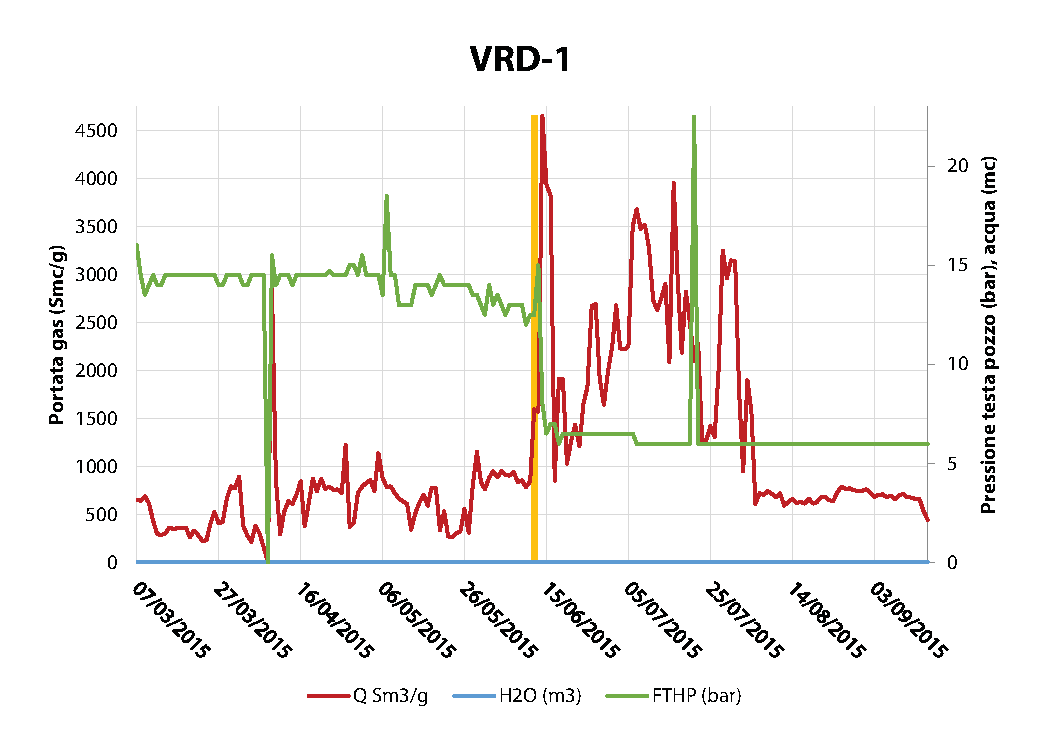
\includegraphics[width=\textwidth]{fig/test/graphs/verdicchio.eps}    \label{fig:test-verdicchio}} \\
\subfloat[][Indici statistici dei parametri relativi al pozzo Verdicchio, periodi 07/03-11/06 e 12/06-16/09.]{
\centering
\footnotesize
\label{tab:verdicchio}
\begin{tabular}{l|crrrr|}
\cline{2-6}
                                 & \textsc{Indice stat.}         & \multicolumn{1}{c}{\textsc{Pre-test}} & \multicolumn{1}{c}{\textsc{Post-test}} & \multicolumn{1}{c}{\(\mathrm{\Delta}\)} & \multicolumn{1}{c|}{\(\mathrm{\Delta}\)\%} \\ \hline
\multicolumn{1}{|l|}{FTHP (bar)} & \(\mu_p\)            & 13,99                                 & 6,41                                   & -7,59                                   & -54,21\%                                    \\
\multicolumn{1}{|l|}{}           & \(\sigma_p\)         & 1,65047                               & 1,91437                                & 0,2639                                  & 15,99\%                                     \\
\multicolumn{1}{|l|}{}           & \(\sigma_p\ast\)     & 11,80\%                                & 29,88\%                                 & 18,09\%                                  & 153,33\%                                    \\ \hline
\multicolumn{1}{|l|}{Gas (Smc)}  & \(\mu_{gas}\)        & 638,622                               & 1605,83                                & 967,211                                 & 151,45\%                                    \\
\multicolumn{1}{|l|}{}           & \(\sigma_{gas}\)     & 355,42                                & 1066,1                                 & 710,678                                 & 199,95\%                                    \\
\multicolumn{1}{|l|}{}           & \(\sigma_{gas}\ast\) & 55,65\%                                & 66,39\%                                 & 10,73\%                                  & 19,29\%                                     \\ \hline
\end{tabular}}
\caption{Valutazione degli effetti dello spiazzamento con schiumogeno sul pozzo Verdicchio, confronto grafico e numerico delle condizioni di produzione precedenti e successive al test.}
\label{fig:vrd-test}
\end{figure}

Il test ha portato a una brusca diminuzione della pressione a testa pozzo, passando da 14 bar a 6,4 bar di media. La pressione di testa pozzo è allineata con quella della linea poiché la duse è totalmente aperta. La variazione del parametro rispecchia fedelmente il cambiamento delle condizioni della linea a valle.\\
La produzione di gas nel secondo periodo è più che raddoppiata, attestandosi a un aumento di portata del 151,45\%. Dopo un primo momento di produzione importante, i valori sono tornati in linea a quelli precedenti alla produzione, ma l'andamento è molto più regolare, con variazioni nell'ordine di decine di Standard metri cubi di gas.\\
I dati di portata del pozzo Verdicchio sono affetti da forte incertezza poiché derivanti da operazioni di stima rispetto la portata totale presso la centrale SGM. Si può comunque affermare che l'applicazione di \textit{foamer} ha decisamente migliorato le condizioni di produzione del pozzo Verdicchio.

\subsection{Campo San Marco}
La \figref{fig:test-campo-snm} rappresenta gli andamenti di portata gas, acqua e pressione in linea del campo SNM sempre relativa all'intervallo di tempo a cavallo del test.

\begin{figure}[htbp]
    \centering
    \subfloat[][Andamento di portata gas, acqua e FLP del campo SNM dal 07/03/2015 al 16/09/2015.]
    {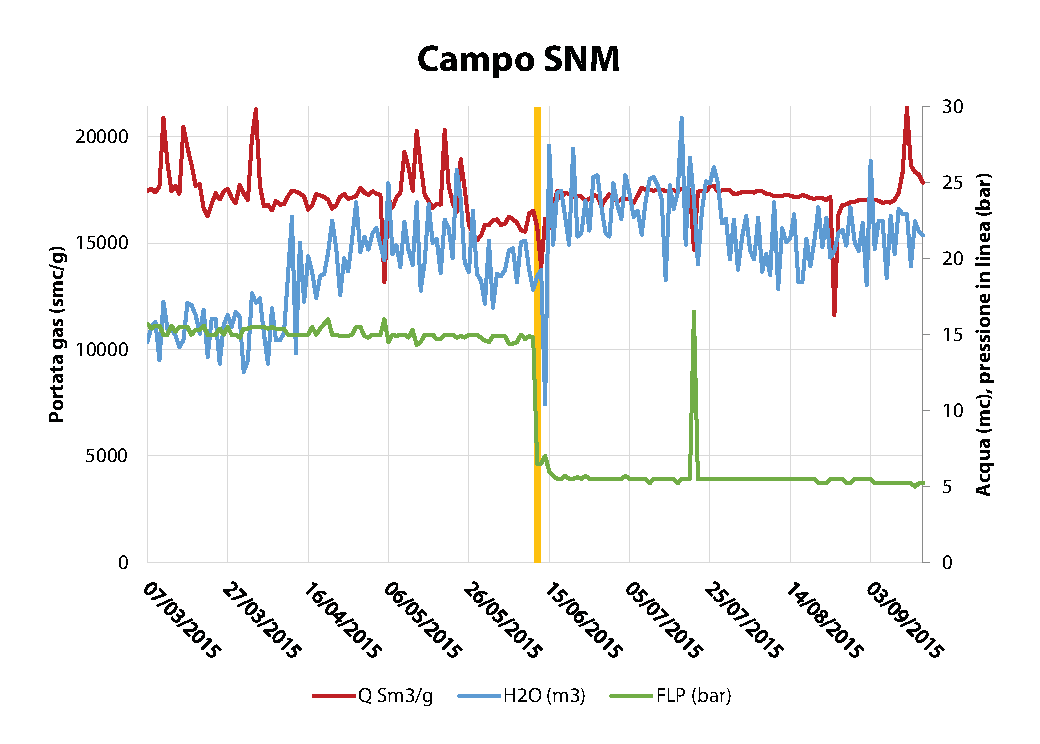
\includegraphics[width=\textwidth]{fig/test/graphs/campo-snm.eps}    \label{fig:test-campo-snm-detail}}\\
\subfloat[][Indici statistici dei parametri relativi al campo SNM, periodi 07/03-11/06 e 12/06-16/09.] {
\centering
\footnotesize
\label{tab:snm}
\begin{tabular}{l|crrrr|}
\cline{2-6}
                                          & Indice stat.         & \multicolumn{1}{c}{\textsc{Pre-test}} & \multicolumn{1}{c}{\textsc{Post-test}} & \multicolumn{1}{c}{\(\mathrm{\Delta}\)} & \multicolumn{1}{c|}{\(\mathrm{\Delta}\)\%} \\ \hline
\multicolumn{1}{|l|}{FTHP (bar)}          & \(\mu_p\)            & 15,00                                 & 5,59                                   & -9,41                                   & -62,74\%                                    \\
\multicolumn{1}{|l|}{}                    & \(\sigma_p\)         & 0,93306435                            & 1,15093355                             & 0,217869                                & 23,35\%                                     \\
\multicolumn{1}{|l|}{}                    & \(\sigma_p\ast\)     & 6,22\%                                 & 20,59\%                                 & 14,37\%                                  & 231,02\%                                    \\ \hline
\multicolumn{1}{|l|}{Gas (Smc)}           & \(\mu_{gas}\)        & 17208,8061                            & 17166,8229                             & -41,98321                               & -0,24\%                                     \\
\multicolumn{1}{|l|}{}                    & \(\sigma_{gas}\)     & 1232,24207                            & 919,781553                             & -312,4605                               & -25,36\%                                    \\
\multicolumn{1}{|l|}{}                    & \(\sigma_{gas}\ast\) & 7,16\%                                 & 5,36\%                                  & -1,80\%                                  & -25,17\%                                    \\ \hline
\multicolumn{1}{|l|}{H\ped{2}O (m\ap{3})} & \(\mu_{H2O}\)     & 18,55                                 & 22,26                                  & 3,71                                    & 20,01\%                                     \\
\multicolumn{1}{|l|}{}                    & \(\sigma_{H2O}\)     & 3,0137599                             & 2,5760467                              & -0,44                                   & -14,52\%                                    \\
\multicolumn{1}{|l|}{}                    & \(\sigma_{H2O}\ast\) & 16,25\%                                & 11,57\%                                 & -4,68\%                                  & -28,77\%                                    \\ \hline
\end{tabular}}
\caption{Valutazione degli effetti dello spiazzamento con schiumogeno sul campo San Marco, confronto grafico e numerico delle condizioni di produzione precedenti e successive al test.}
\label{fig:test-campo-snm}
\end{figure}

La contropressione si è abbassata notevolmente, infatti si è passati da una pressione in linea di circa 15 bar a una media di 5,5 bar (nell'ultimo periodo il valore è costante, 5,2 bar). La dispersione dei valori di pressione è maggiore nel secondo periodo:  l'effetto tende però a diminuire nel tempo, come visibile nella parte destra del grafico. È importare sottolineare il fatto che la pressione che governa la testa pozzo è quella valvole di regolazione (PCV, Pressure Control Valve), regolata prima del test a 15 bar, successivamente a 11 bar e infine 9 bar.\\
La produzione del gas non ha subito variazioni e la media è rimasta più o meno costante. Tuttavia la portata ha acquisito un andamento più lineare e costante, testimoniato dal decrescita del coefficiente di variazione rispetto al primo periodo del -25,17\% \\
La produzione di acqua è aumentata del 20\%, aumentando anche l’oscillazione attorno il valore medio. Anche l'acqua, come la produzione di gas, sembra essersi stabilizzata, come dimostra la variazione del coefficiente di variazione tra il primo e il secondo scenario (-18,77\%).\\
A distanza di più di tre mesi dall'applicazione, non sono stati ancora impiegati stick nei pozzi del campo San Marco, applicazione che veniva effettuata sporadicamente a distanza di qualche settimana.\\
Scendendo nel dettaglio, si sono valutati i singoli pozzi del campo SNM. I pozzi SM2B e SM3B sono quelli che contribuiscono maggiormente alla produzione totale di gas del campo. Entrambi i pozzi hanno reagito all'applicazione in modo positivo, come testimoniano la \figref{fig:test-sm2b} e la \figref{fig:test-sm3b}. In questi pozzi si ha un lieve aumento di produzione nell'ordine di qualche punto percentuale. La diminuzione di pressione è sempre fedele al settaggio della PCV della linea di mandata. La produzione di acqua è fortemente aumentata, attestandosi addirittura a un incremento del 31,86\% per quanto riguarda il pozzo SM2B.

\begin{figure}[htbp]
    \centering
    \subfloat[][Andamento di portata gas, acqua e FLP del pozzo SM2B appartentente al campo San Marco, dal 07/03/2015 al 16/09/2015.]
    {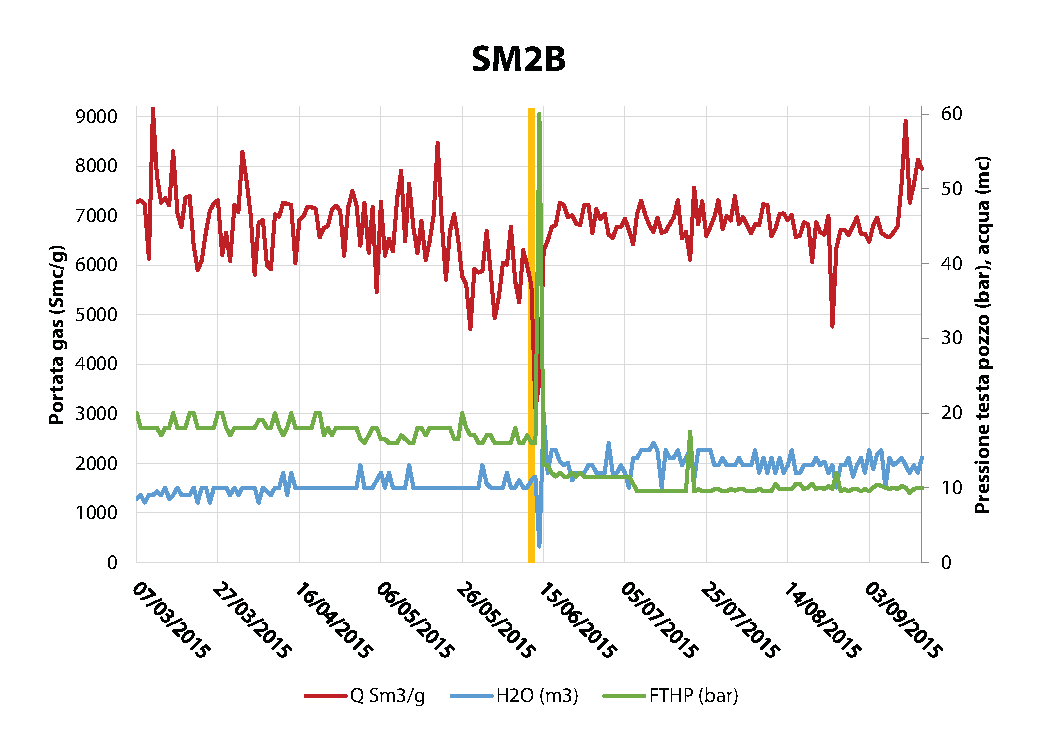
\includegraphics[width=\textwidth]{fig/test/graphs/sm2b.eps}
    \label{fig:test-sm2b-detail}}\\
\subfloat[][Indici statistici dei parametri relativi al pozzo SM2B, periodi 07/03-11/06 e 12/06-16/09.] {
\centering
\footnotesize
\label{tab:sm2b}
\begin{tabular}{l|crrrr|}
\cline{2-6}
                                          & Indice stat.         & \multicolumn{1}{c}{\textsc{Pre-test}} & \multicolumn{1}{c}{\textsc{Post-test}} & \multicolumn{1}{c}{\(\mathrm{\Delta}\)} & \multicolumn{1}{c|}{\(\mathrm{\Delta}\)\%} \\ \hline
\multicolumn{1}{|l|}{FTHP (bar)}          & \(\mu_p\)            & 17,69                                 & 10,91                                  & -6,79                                   & -38,35\%                                    \\
\multicolumn{1}{|l|}{}                    & \(\sigma_p\)         & 1,14566                               & 5,2287                                 & 4,08304                                 & 356,39\%                                    \\
\multicolumn{1}{|l|}{}                    & \(\sigma_p\ast\)     & 6,47\%                                 & 47,93\%                                 & 41,46\%                                  & 640,29\%                                    \\ \hline
\multicolumn{1}{|l|}{Gas (Smc)}           & \(\mu_{gas}\)        & 6714,82                               & 6802,47                                & 87,6524                                 & 1,31\%                                      \\
\multicolumn{1}{|l|}{}                    & \(\sigma_{gas}\)     & 764,029                               & 675,602                                & -88,4269                                & -11,57\%                                    \\
\multicolumn{1}{|l|}{}                    & \(\sigma_{gas}\ast\) & 11,38\%                                & 9,93\%                                  & -1,45\%                                  & -12,71\%                                    \\ \hline
\multicolumn{1}{|l|}{H\ped{2}O (m\ap{3})} & \(\mu_{H2O}\)     & 9,98                                  & 13,17                                  & 3,18                                    & 31,86\%                                     \\
\multicolumn{1}{|l|}{}                    & \(\sigma_{H2O}\)     & 0,92624                               & 1,88787                                & 0,96                                    & 103,82\%                                    \\
\multicolumn{1}{|l|}{}                    & \(\sigma_{H2O}\ast\) & 9,28\%                                 & 14,34\%                                 & 5,06\%                                   & 54,57\%                                     \\ \hline
\end{tabular}}
\caption{Valutazione degli effetti dello spiazzamento con schiumogeno sul pozzo SM2B del campo San Marco, confronto grafico e numerico delle condizioni di produzione precedenti e successive al test.}
\label{fig:test-sm2b}
\end{figure}

\begin{figure}[htbp]
    \centering
    \subfloat[][Andamento di portata gas, acqua e FLP del pozzo SM3B appartenente al campo San Marco, dal 07/03/2015 al 16/09/2015.]
    {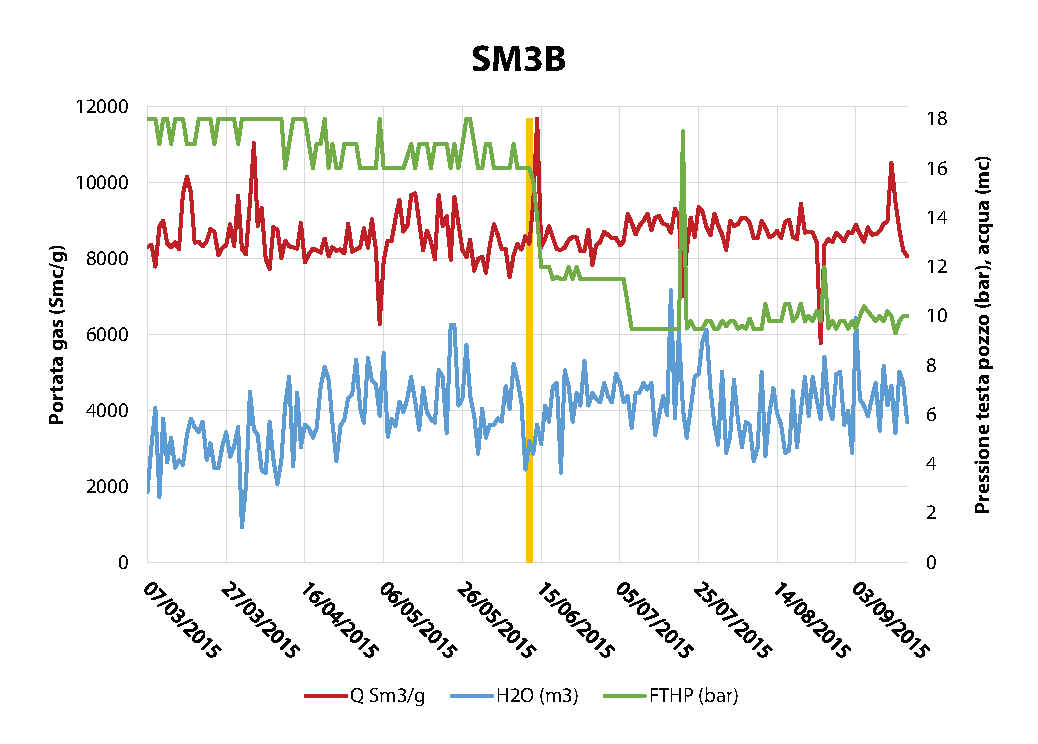
\includegraphics[width=\textwidth]{fig/test/graphs/sm3b.eps}\label{fig:test-sm3b-detail}}\\
\subfloat[][Indici statistici dei parametri relativi al pozzo SM3B, periodi 07/03-11/06 e 12/06-16/09.] {
\centering
\footnotesize
\label{tab:sm3b}
\begin{tabular}{l|crrrr|}
\cline{2-6}
                                          & Indice stat.         & \multicolumn{1}{c}{\textsc{Pre-test}} & \multicolumn{1}{c}{\textsc{Post-test}} & \multicolumn{1}{c}{\(\mathrm{\Delta}\)} & \multicolumn{1}{c|}{\(\mathrm{\Delta}\)\%} \\ \hline
\multicolumn{1}{|l|}{FTHP (bar)}          & \(\mu_p\)            & 17,05                                 & 10,40                                  & -6,65                                   & -38,99\%                                    \\
\multicolumn{1}{|l|}{}                    & \(\sigma_p\)         & 0,83137                               & 1,29765                                & 0,46628                                 & 56,09\%                                     \\
\multicolumn{1}{|l|}{}                    & \(\sigma_p\ast\)     & 4,88\%                                 & 12,48\%                                 & 7,60\%                                   & 155,86\%                                    \\ \hline
\multicolumn{1}{|l|}{Gas (Smc)}           & \(\mu_{gas}\)        & 8530,23                               & 8712,95                                & 182,713                                 & 2,14\%                                      \\
\multicolumn{1}{|l|}{}                    & \(\sigma_{gas}\)     & 628,882                               & 592,611                                & -36,2704                                & -5,77\%                                     \\
\multicolumn{1}{|l|}{}                    & \(\sigma_{gas}\ast\) & 7,37\%                                 & 6,80\%                                  & -0,57\%                                  & -7,74\%                                     \\ \hline
\multicolumn{1}{|l|}{H\ped{2}O (m\ap{3})} & \(\mu_{H2O}\)        & 5,73                                  & 6,48                                   & 0,75                                    & 13,08\%                                     \\
\multicolumn{1}{|l|}{}                    & \(\sigma_{H2O}\)     & 1,50841                               & 1,30903                                & -0,20                                   & -13,22\%                                    \\
\multicolumn{1}{|l|}{}                    & \(\sigma_{H2O}\ast\) & 26,33\%                                & 20,21\%                                 & -6,12\%                                  & -23,26\%                                    \\ \hline
\end{tabular}}
\caption{Valutazione degli effetti dello spiazzamento con schiumogeno sul pozzo SM3B del campo San Marco, confronto grafico e numerico delle condizioni di produzione precedenti e successive al test.}
\label{fig:test-sm3b}
\end{figure}

\clearpage

%---------------------------------------------

\subsection{Analisi costi e benefici}
In \tabref{tab:test-costi} sono stati calcolati i costi associati al test e successivamente i ricavi e i costi variabili dei due scenari presi in considerazione al fine di poter calcolare così il margine finale acquisito tramite l'applicazione.

\begin{table}[htbp]
\centering
\footnotesize
\caption{Calcolo costi associati all'applicazione di schiumogeno.}
\label{tab:test-costi}
\begin{tabular}{|l|r|}
\hline
Consumo schiuma                     & 133 l                                 \\
Consumo antischiuma                 & 150 l                                     \\
Costo unitario schiuma              & 5,2 €/kg                                   \\
Costo unitario antisch.             & 4,8 €/kg                                   \\ 
\textbf{Costo  iniezione}           & {\color[HTML]{CB0000} € 1.447,69}          \\ \hline
\textbf{Costo smalt. acqua}         & 7,47 €/ton                                 \\
\textbf{Volume acqua stimata}       & 12,74 m\ap{3}                                   \\
\textbf{Costo tot agg. smaltimento} & {\color[HTML]{CB0000} \textbf{€ 95,17}}    \\ \hline
\textbf{\textsc{Costo tot.}}                 & {\color[HTML]{CB0000} \textbf{€ 1.542,86}} \\ \hline
\end{tabular}
\end{table}

L'analisi dei due diversi scenari in \tabref{tab:guadagno} è stata eseguita calcolando il ricavo della produzione di gas, il costo di smaltimento dell'acqua prodotta (costo variabile) e il costo dell'iniezione (costo fisso), non presente quindi nel primo periodo di riferimento. Si è considerato un prezzo medio di vendita del gas di 0,25 €/Smc.

\begin{table}[htbp]
\centering
\footnotesize
\caption{Analisi guadagno nei due diversi scenari pre- e post-test.}
\label{tab:guadagno}
\begin{tabular}{lrr}
\cline{2-3}
\multicolumn{1}{l|}{}                    & \multicolumn{1}{l|}{\textsc{Pre-test (07/03-11/06)}}              & \multicolumn{1}{l|}{\textsc{Post-test (12/06-16/09)}}             \\ \hline
\multicolumn{1}{|l|}{Ricavo gas}         & \multicolumn{1}{r|}{€ 432.919,25}                        & \multicolumn{1}{r|}{€ 454.886,50}                        \\
\multicolumn{1}{|l|}{Costo smalt. acqua} & \multicolumn{1}{r|}{{\color[HTML]{CB0000} -€ 13.437,96}} & \multicolumn{1}{r|}{{\color[HTML]{CB0000} -€ 16.103,64}} \\
\multicolumn{1}{|l|}{Costo test}         & \multicolumn{1}{r|}{€ 0,00}                              & \multicolumn{1}{r|}{-€ 1.542,86}                         \\
\multicolumn{1}{|l|}{Costi tot.}         & \multicolumn{1}{r|}{{\color[HTML]{CB0000} -€ 13.437,96}} & \multicolumn{1}{r|}{{\color[HTML]{CB0000} -€ 17.646,50}} \\
\multicolumn{1}{|l|}{\textbf{TOT.}}      & \multicolumn{1}{r|}{\textbf{€ 419.481,29}}               & \multicolumn{1}{r|}{\textbf{€ 437.240,00}}               \\ \hline
\textbf{}                                & \multicolumn{1}{l}{}                                     & \multicolumn{1}{l}{}                                     \\
\textbf{}                                & \multicolumn{1}{l}{\textbf{}}                            & \multicolumn{1}{l}{}                                     \\
\textbf{}                                & \multicolumn{1}{l}{\textbf{}}                            & \multicolumn{1}{l}{}                                    
\end{tabular}
\end{table}

L'applicazione del foamer in linea si è concretizzata con un aumento del margine di 17.758,72 €, con un giornaliero di 1.182,91 €/g. L'aumento di margine percentuale è pari al 4,23\%. L'incremento di ricavo legato alla produzione di gas di 8.342 € è netto rispetto all'aumento dei costi totali pari a 4.208,53 €. Importante considerazione va fatta sulla rapporto costi fissi-costi variabili: la spesa relativa a foamer e defoamer rappresenta l'8,74\% dei costi totali (non è apprezzabile in \figref{fig:costi-benefici}), a conferma delle maggiori potenzialità economiche dell'applicazione per volumi di gas maggiori.\\

\begin{figure}[htbp]
    \centering
    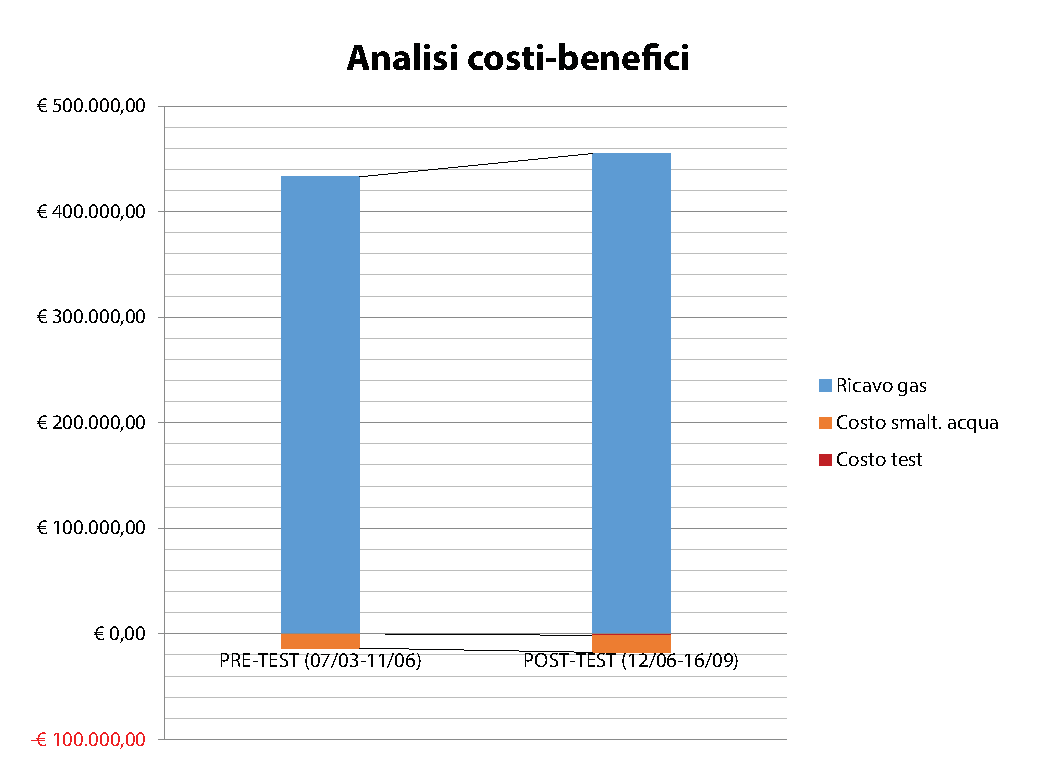
\includegraphics[width=\textwidth]{fig/test/graphs/costi-benefici.eps}
    \caption{Analisi costi e ricavi per i due rispettivi scenari di riferimento.} 
    \label{fig:costi-benefici}
\end{figure}


\subsection{Piggaggio della linea di produzione}
Come detto in precedenza l'intera applicazione si è basata sulle conoscenze acquisite con l'applicazione di schiumogeno in pozzo e sui valori relativi ai \textit{pigging} sulla condotta di Verdicchio svolti in precedenza.\\
L'ultima operazione di piggaggio della linea di Verdicchio è stata effettuata il 30 luglio 2013. L'applicazione è stata eseguita in concomitanza di una riparazione alla condotta resasi necessaria in seguito a un danno arrecato durante degli interventi sulla rete fognaria adiacente. Il giorno 28 luglio 2015 è stata fermata la produzione ed la condotta è stata bonificata tramite l'iniezione di azoto. In seguito sono cominciate le operazioni di riparazione, durate due giorni.\\
Il 30 luglio 2013 è stata effettuata l'operazione di piggaggio della linea. L'operazione ha avuto come fine la pulizia della condotta in seguito agli interventi di riparazione e lo spiazzamento dell'acqua collocata in particolare negli avvallamenti. L'utensile impiegato è stato uno scovolo a mandrino dotato di spazzole pulenti, dischi di supporto e guarnizioni a tazza per la tenuta idraulica e la propulsione. Lo strumento era inoltre dotato di segnalatore elettronico, il quale segnalava la posizione lungo la condotta tramite degli indicatori di posizione installati sulle canalette di intercetto. Il mezzo di propulsione impiegato è azoto. Lo scovolo è stato inviato dalla trappola di lancio del campo Verdicchio (\figref{fig:test-trappola}) ed è giunto alla trappola di ricezione della centrale SGM.

\begin{figure}[htbp]
\centering
\subfloat[][Vista laterale.]
{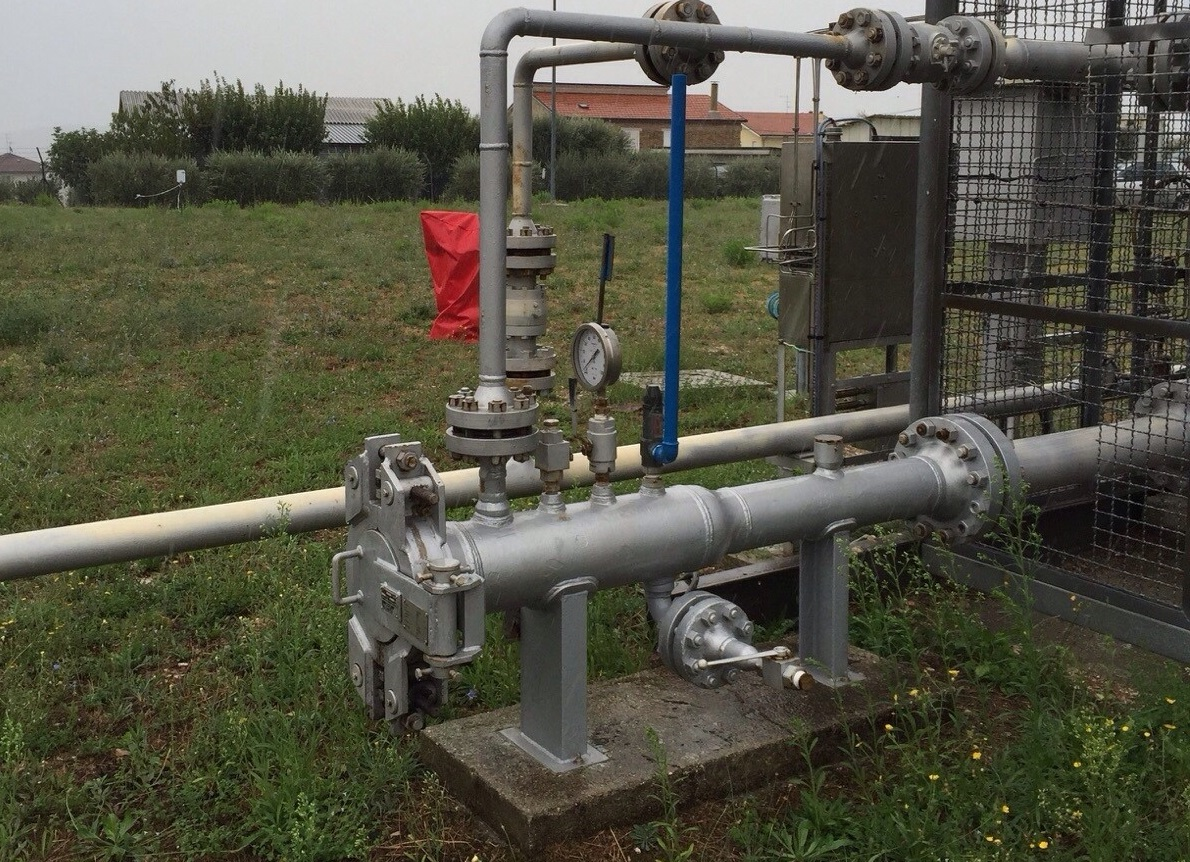
\includegraphics[height=.28\textheight]{fig/test/trappola-1} \label{fig:trappola-1}} \qquad
\subfloat[][Vista frontale.]
{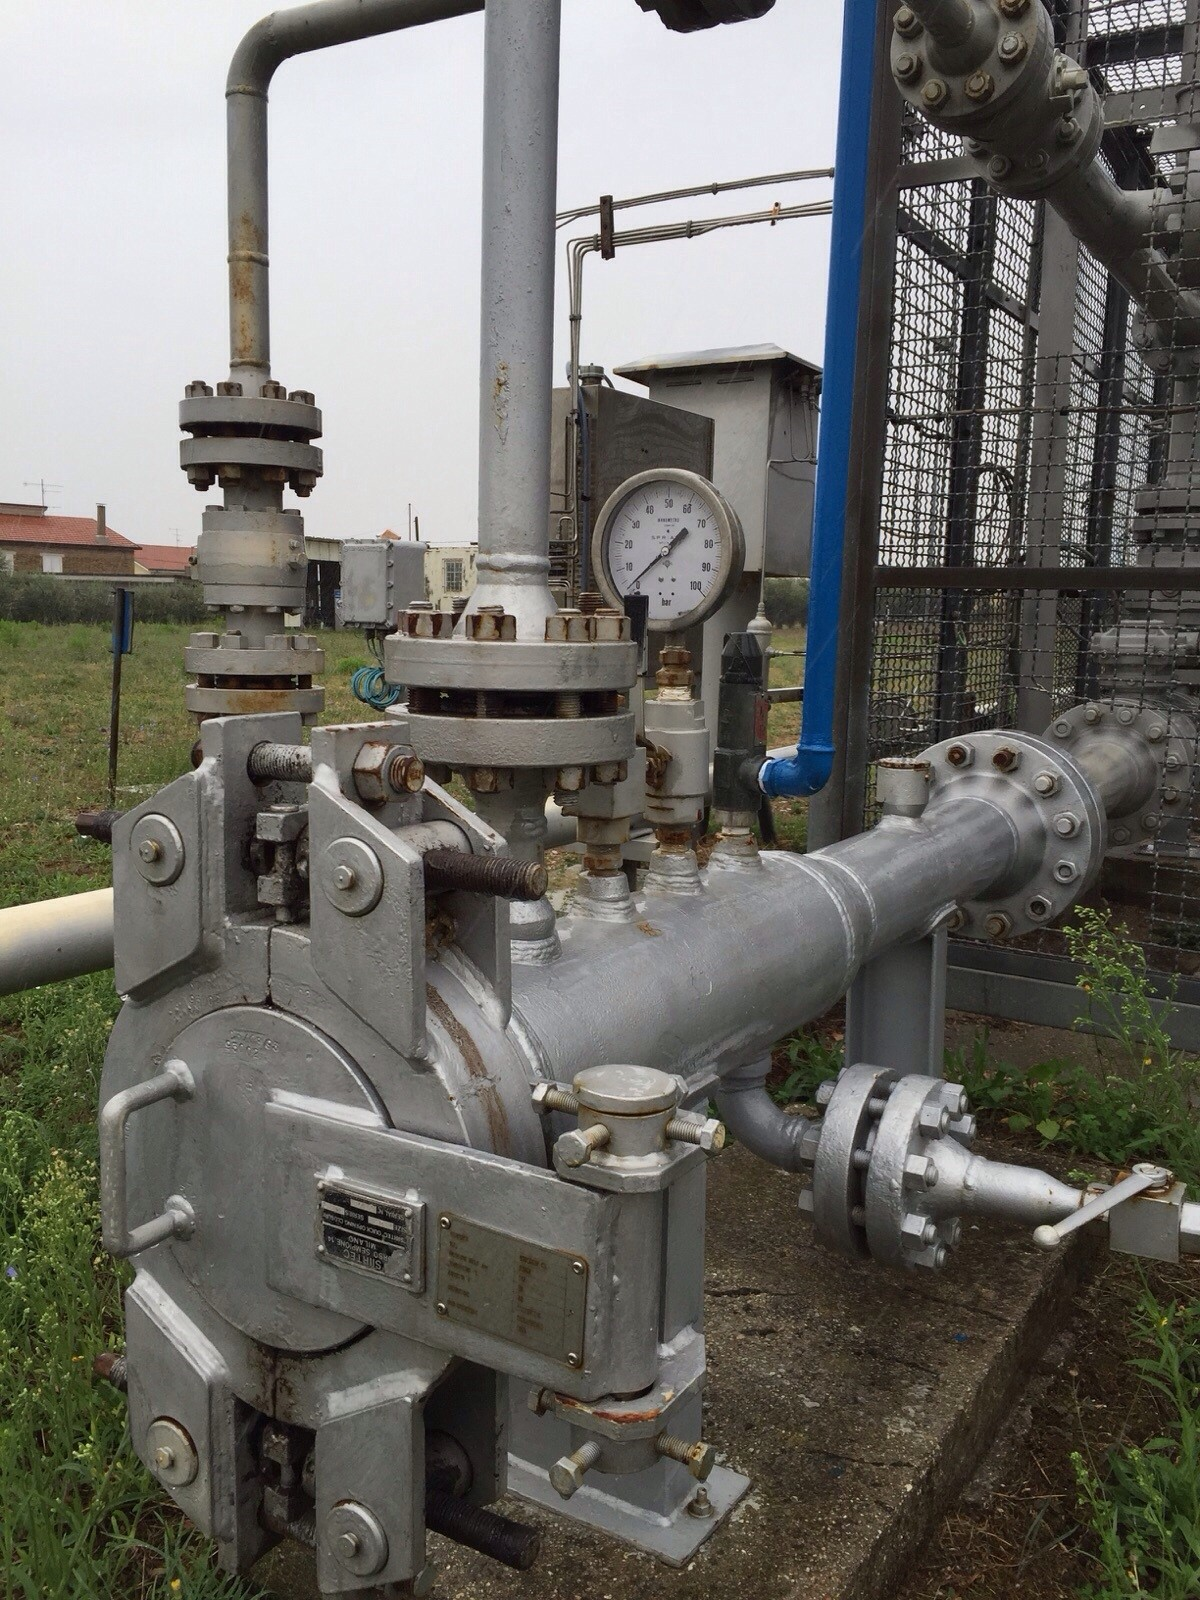
\includegraphics[height=.28\textheight]{fig/test/trappola-2} \label{fig:trappola-2}}
\caption{Trappola di lancio del campo Verdicchio.}
\label{fig:test-trappola}
\end{figure}

L'operazione ha avuto durata complessiva di 6 ore, l'acqua spiazzata è stata di circa 14,5 m\ap{3}, valore in linea con l'acqua spiazzata tramite l'utilizzo dello schiumogeno. Al termine dell'operazione è stata riavviata la produzione in linea e si è proceduto allo spurgo della linea: il gas è stato convogliato alla torcia fredda fintanto che i valori di gas metano non hanno raggiunto nuovamente il 98\%. Durante il \textit{pigging} non è stato possibile rilevare la posizione dello scovolo lungo la condotta, a causa della rottura immediata del dispositivo di segnalazione una volta lanciato dalla trappola.\\
Il 2 agosto è stato effettuato un altro lancio di \textit{pig}, questa volta uno scovolo in schiuma solida con rivestimento in poliuretano, la quale ha permesso il recupero dei frammenti del dispositivo di rilevazione e un'ulteriore deidratazione. La propulsione è sempre avvenuta per mezzo gassoso (azoto) e ha richiesto bonifica e spurgo rispettivamente prima e dopo il lancio dello scovolo.\\
La \figref{fig:test-pig2013} mostra l'andamento dei parametri di gas, pressione in linea e acqua prodotta della linea di San Marco. L'intervallo di tempo scelto va dal 24 aprile 2015 al 3 novembre 2013: come per la valutazione dell'efficacia dello schiumogeno, 97 giorni prima e dopo il piggaggio della linea. Nonostante gli indici statistici siano stati proposti anche in questa occasione, non consentono di acquisire informazioni aggiuntive poiché sono fortemente influenzati dall'interruzione della linea di quattro giorni utile alla riparazione della condotta con doppio piggaggio (dal 28 luglio al 2 agosto 2013) e ai controlli decennali di tenuta idraulica degli impianti di San Marco (dal 7 al 19 ottobre 2013).
\begin{figure}[htbp]
    \centering
    \subfloat[][Andamento di portata gas, acqua e FLP del campo San Marco, dal 24/04/2013 al 03/11/2013.]
    {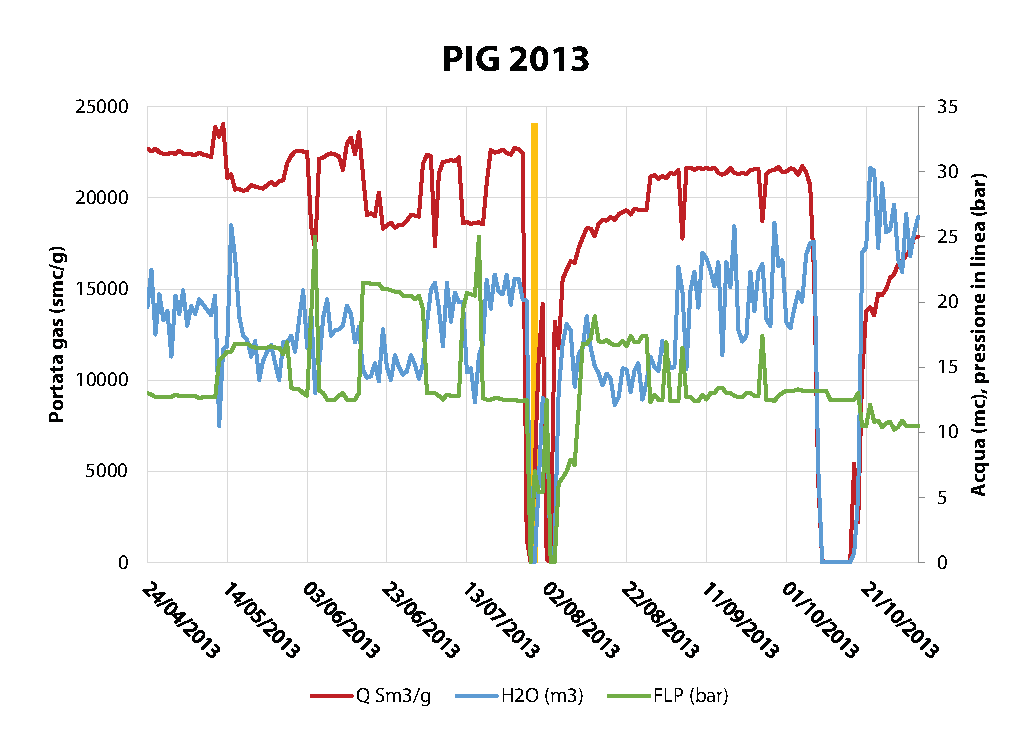
\includegraphics[width=\textwidth]{fig/test/graphs/pig2013.eps}\label{fig:test-pig2013-detail}}\\
\subfloat[][Indici statistici dei parametri relativi al campo San Marco, periodi 24/04/2013-29/07/2013 e 30/07/2013-03/11/2013.] {
\centering
\footnotesize
\begin{tabular}{l|crrrr|}
\cline{2-6}
                                          & \textsc{Indice stat.} & \multicolumn{1}{c}{\textsc{Pre-pig}} & \multicolumn{1}{c}{\textsc{Post-pig}} & \multicolumn{1}{c}{\(\mathrm{\Delta}\)} & \multicolumn{1}{c|}{\(\mathrm{\Delta}\)\%} \\ \hline
\multicolumn{1}{|l|}{FTHP (bar)}          & \(\mu_p\)             & 15,18                                & 12,63                                 & -2,55                                   & -16,82\%                                    \\
\multicolumn{1}{|l|}{}                    & \(\sigma_p\)          & 3,91490272                           & 3,32412879                            & -0,590774                               & -15,09\%                                    \\
\multicolumn{1}{|l|}{}                    & \(\sigma_p\ast\)      & 25,79\%                               & 26,32\%                                & 0,54\%                                   & 2,08\%                                      \\ \hline
\multicolumn{1}{|l|}{Gas (Smc)}           & \(\mu_{gas}\)         & 20652,9082                           & 16487,9479                            & -4164,96                                & -20,17\%                                    \\
\multicolumn{1}{|l|}{}                    & \(\sigma_{gas}\)      & 3720,93721                           & 6792,04273                            & 3071,106                                & 82,54\%                                     \\
\multicolumn{1}{|l|}{}                    & \(\sigma_{gas}\ast\)  & 18,02\%                               & 41,19\%                                & 23,18\%                                  & 128,65\%                                    \\ \hline
\multicolumn{1}{|l|}{H\ped{2}O (m\ap{3})} & \(\mu_{H2O}\)         & 17,53                                & 16,90                                 & -0,63                                   & -3,61\%                                     \\
\multicolumn{1}{|l|}{}                    & \(\sigma_{H2O}\)      & 3,73482088                           & 7,8300456                             & 4,10                                    & 109,65\%                                    \\
\multicolumn{1}{|l|}{}                    & \(\sigma_{H2O}\ast\)  & 21,30\%                               & 46,33\%                                & 25,03\%                                  & 117,50\%                                    \\ \hline
\end{tabular}}
\caption{Valutazione degli effetti dello spiazzamento con piggaggio sul sul campo San Marco, confronto grafico e numerico delle condizioni di produzione precedenti e successive al \textit{pigging}.}
\label{fig:test-pig2013}
\end{figure}

Prima del piggaggio la produzione oscillava sensibilmente attorno ai 22 {Smc}/g, con una produzione di acqua attorno ai 12 m\ap{3}/g e la pressione della linea che si aggira attorno ai 13 bar. Le variazioni nette dei parametri presenti sono da ricollegare agli interventi alla centrale SGM: a volte la produzione è stata fermata oppure si è operato in condizioni di alta pressione. Di conseguenza in corrispondenza di picchi di alta pressione si ha una minore produzione. Questa relazione comunque continua a confermare come la produzione sia profondamente legata ai valori di contropressione a valle.\\
Dopo l'applicazione del piggaggio la produzione è tornata lentamente ai valori originali solo dopo 30 giorni. Ciò testimonia il fatto di come i pozzi abbiano inerzia propria e al fine di mantenere delle condizioni costanti di produzione vanno evitati lunghe interruzioni.\\
La pressione in linea è cambiata solo momentaneamente: se la pressione era diminuita fino a 6,5 bar a distanza di sei giorni dal piggaggio e quattro giorni dall'avvio della produzione, questo valore è aumentato velocemente e dopo appena 10 giorni la pressione in linea è tornata a circa 12 bar: il piggaggio sembra che in qualche modo non abbia funzionato correttamente oppure non garantisce un efficacia di spiazzamento sufficiente.\\
L'aumento di acqua prodotta è consistente, oscilla attorno ai 25 m\ap{3}/g, con un aumento quindi di 3 m\ap{3} giornalieri.\\



\subsection{Interpretazione delle condizioni di flusso}
I risultati ottenuti dal testo hanno portato alla conclusione che il principio alla base del test non sia la diminuzione della tensione superficiale, bensì la creazione di un "pig" chimico stabile lungo tutto il tragitto, capace di spiazzare l'acqua da tutta la condotta. L'ipotesi viene confermata dall'ingente volume d'acqua giunto alla centrale SGM: più del 50\% del volume totale in circa 10 minuti.\\
Il fenomeno può essere spiegato da due condizioni iniziali:
\begin{itemize}
\item \textbf{composizione}: l'introduzione di foamer e acqua contemporaneamente del volume di mandata ha fatto sì che si creasse un fronte di schiuma già alla mandata;
\item \textbf{geometria}: sulla mandata di SNM, praticamente a valle di tutto il volume di batch, è presente una valvola di regolazione Fisher, la quale agisce su un Venturi. La valvola aumenta così la velocità del fluido, quindi le turbolenze, generando un fronte di schiuma ad alta velocità, capace di spiazzare l'acqua nelle condotte;
\item \textbf{pressione}: l'interruzione della linea e la depressurizzazione del tratto di linea interessato dall'applicazione ha permesso un incremento della variazione di pressione, con l'aumento di efficacia della Fisher sulla generazione del fronte compatto di schiuma.\\
\end{itemize}



\clearpage{\pagestyle{empty}\cleardoublepage}